% Options for packages loaded elsewhere
\PassOptionsToPackage{unicode}{hyperref}
\PassOptionsToPackage{hyphens}{url}
%
\documentclass[
  oneside]{book}
\usepackage{amsmath,amssymb}
\usepackage{lmodern}
\usepackage{iftex}
\ifPDFTeX
  \usepackage[T1]{fontenc}
  \usepackage[utf8]{inputenc}
  \usepackage{textcomp} % provide euro and other symbols
\else % if luatex or xetex
  \usepackage{unicode-math}
  \defaultfontfeatures{Scale=MatchLowercase}
  \defaultfontfeatures[\rmfamily]{Ligatures=TeX,Scale=1}
\fi
% Use upquote if available, for straight quotes in verbatim environments
\IfFileExists{upquote.sty}{\usepackage{upquote}}{}
\IfFileExists{microtype.sty}{% use microtype if available
  \usepackage[]{microtype}
  \UseMicrotypeSet[protrusion]{basicmath} % disable protrusion for tt fonts
}{}
\makeatletter
\@ifundefined{KOMAClassName}{% if non-KOMA class
  \IfFileExists{parskip.sty}{%
    \usepackage{parskip}
  }{% else
    \setlength{\parindent}{0pt}
    \setlength{\parskip}{6pt plus 2pt minus 1pt}}
}{% if KOMA class
  \KOMAoptions{parskip=half}}
\makeatother
\usepackage{xcolor}
\usepackage{longtable,booktabs,array}
\usepackage{calc} % for calculating minipage widths
% Correct order of tables after \paragraph or \subparagraph
\usepackage{etoolbox}
\makeatletter
\patchcmd\longtable{\par}{\if@noskipsec\mbox{}\fi\par}{}{}
\makeatother
% Allow footnotes in longtable head/foot
\IfFileExists{footnotehyper.sty}{\usepackage{footnotehyper}}{\usepackage{footnote}}
\makesavenoteenv{longtable}
\usepackage{graphicx}
\makeatletter
\def\maxwidth{\ifdim\Gin@nat@width>\linewidth\linewidth\else\Gin@nat@width\fi}
\def\maxheight{\ifdim\Gin@nat@height>\textheight\textheight\else\Gin@nat@height\fi}
\makeatother
% Scale images if necessary, so that they will not overflow the page
% margins by default, and it is still possible to overwrite the defaults
% using explicit options in \includegraphics[width, height, ...]{}
\setkeys{Gin}{width=\maxwidth,height=\maxheight,keepaspectratio}
% Set default figure placement to htbp
\makeatletter
\def\fps@figure{htbp}
\makeatother
\setlength{\emergencystretch}{3em} % prevent overfull lines
\providecommand{\tightlist}{%
  \setlength{\itemsep}{0pt}\setlength{\parskip}{0pt}}
\setcounter{secnumdepth}{5}
\usepackage{booktabs}

\usepackage{fontspec} % Font selection for XeLaTeX; see fontspec.pdf for documentation
\defaultfontfeatures{Mapping=tex-text} % to support TeX conventions like ``---''
\usepackage{xunicode} % Unicode support for LaTeX character names (accents, European chars, etc)
\usepackage{xltxtra} % Extra customizations for XeLaTeX

\setmainfont{Crimson Pro} % set the main body font (\textrm), assumes Charis SIL is installed
\setsansfont{Source Sans Pro}
\setmonofont{Ubuntu Mono}

% \renewcommand{\topfraction}{.85}
% \renewcommand{\bottomfraction}{.7}
% \renewcommand{\textfraction}{.15}
% \renewcommand{\floatpagefraction}{.66}
% \setcounter{topnumber}{3}
% \setcounter{bottomnumber}{3}
% \setcounter{totalnumber}{4}

% \usepackage{float}
% \let\origfigure\figure
% \let\endorigfigure\endfigure
% \renewenvironment{figure}[1][2] {
%     \expandafter\origfigure\expandafter[H]
% } {
%     \endorigfigure
% }
\usepackage{flafter}
\usepackage{booktabs}
\usepackage{longtable}
\usepackage{array}
\usepackage{multirow}
\usepackage{wrapfig}
\usepackage{float}
\usepackage{colortbl}
\usepackage{pdflscape}
\usepackage{tabu}
\usepackage{threeparttable}
\usepackage{threeparttablex}
\usepackage[normalem]{ulem}
\usepackage{makecell}
\usepackage{xcolor}
\usepackage{siunitx}

  \newcolumntype{d}{S[
    input-open-uncertainty=,
    input-close-uncertainty=,
    parse-numbers = false,
    table-align-text-pre=false,
    table-align-text-post=false
  ]}
  
\ifLuaTeX
  \usepackage{selnolig}  % disable illegal ligatures
\fi
\usepackage[]{natbib}
\bibliographystyle{apalike}
\IfFileExists{bookmark.sty}{\usepackage{bookmark}}{\usepackage{hyperref}}
\IfFileExists{xurl.sty}{\usepackage{xurl}}{} % add URL line breaks if available
\urlstyle{same} % disable monospaced font for URLs
\hypersetup{
  pdftitle={Health Policy Reform in the 50 States, 2011-2022},
  pdfauthor={Boris Shor},
  hidelinks,
  pdfcreator={LaTeX via pandoc}}

\title{Health Policy Reform in the 50 States, 2011-2022}
\author{Boris Shor}
\date{2022-11-23}

\begin{document}
\maketitle

{
\setcounter{tocdepth}{1}
\tableofcontents
}
\hypertarget{abstract}{%
\chapter{Abstract}\label{abstract}}

This book describes and analyzes health policy reforms from 2011-2022. It is funded by the Russell Sage Foundation.

How well do the America's thousands of state legislators represent their constituents on the implementation of health policy reform at the state level? Are the decisions they make in the statehouse reflective of the wishes and needs of their constituents, or do other influences such as their own preferences, or those of their party hold more sway? We don't now know this because of huge problems in measurement, especially at this level of government. Understanding the receptiveness of state legislators individuals and in aggregate to such varied influence will help us to predict the course of coalitions that can be constructed in each state to pass a diverse set of health reform policies.

\hypertarget{intro}{%
\chapter{Introduction}\label{intro}}

\hypertarget{congress}{%
\section{Congress}\label{congress}}

The summer of 2017 was marked by the dramatic meltdown of Republican ``repeal and replace'' legislation in Congress. A major political development that played a part was the significant rise in public approval for the Affordable Care Act. Prior to 2017, numerous surveys (including the Kaiser Family Foundation tracking polls) have shown that nearly all elements within ``Obamacare'' have vast majorities in favor, at the same time as support for the law overall remained polarized. That changed with the introduction of concrete Republican legislation to overturn the ACA, when overall favorability climbed well into majoritarian terrain. Even Republican identifiers in surveys gave dismal ratings to the Republican leadership and its legislation. The disjuncture between national Republican attempts to overturn the Affordable Care Act and public support for it is striking, especially given older evidence of responsiveness in health policy spending \citep{Soroka:2003, Wlezien:2004}.

\hypertarget{public-opinion}{%
\section{Public Opinion}\label{public-opinion}}

When Americans are asked which party they trust to enact health care policy, they disproportionately say (in national samples) they trust the Democratic party.

\begin{figure}
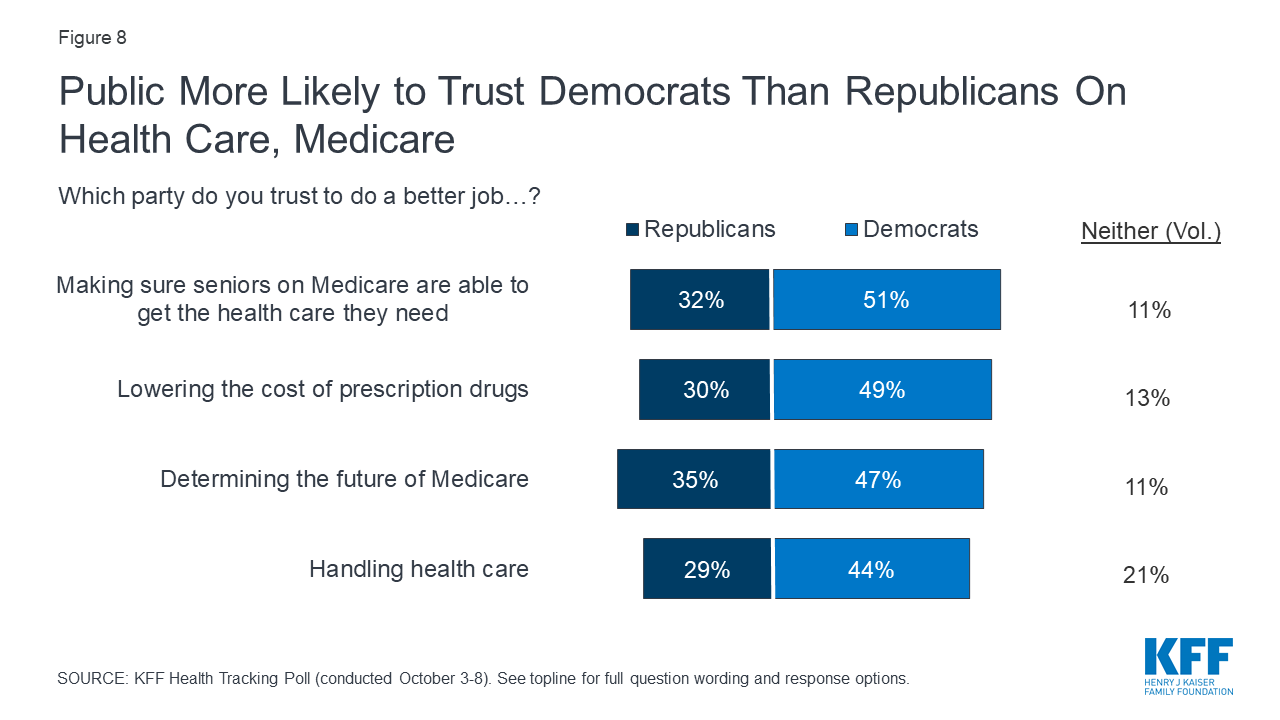
\includegraphics[width=0.99\linewidth]{Plots/Web/party_trust_healthcare} \caption{Issue Ownership of Health Care}\label{fig:pew-health-ownership}
\end{figure}

When the Affordable Care Act was passed, it was deeply polarized in public opinion. That has changed, with the ACA now (nationally) leading in support.

\begin{figure}
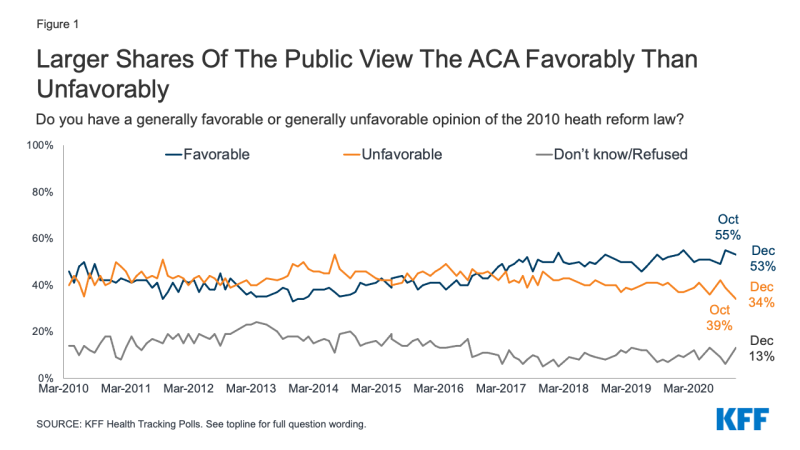
\includegraphics[width=0.99\linewidth]{Plots/Web/aca_favor_dec20} \caption{Affordable Care Act Approval}\label{fig:kff-aca}
\end{figure}

\hypertarget{state-examples}{%
\section{State Examples}\label{state-examples}}

\hypertarget{the-latecomers-medicaid-expansion-in-virginia-and-montana}{%
\subsection{The Latecomers: Medicaid expansion in Virginia and Montana}\label{the-latecomers-medicaid-expansion-in-virginia-and-montana}}

\hypertarget{virginia}{%
\subsubsection{Virginia}\label{virginia}}

Virginia Voters in November 2017 dealt a stunning blow to Republicans who controlled both chambers of the state legislature. The previous Republican-controlled legislature had been instrumental in blocking Medicaid expansion in the state despite a Democratic governor who strongly supported it, and statewide public opinion which also was significantly in favor. Yet Republicans retained a bare majority in the House of Delegates, and still controlled the State Senate. But individual Republicans including State Senators Frank Wagner and Emmet Hanger Jr., and Delegates Chris Peace and Terry Kilgore, changed their position on expansion and created a coalition with the Democratic minority to successfully pass Medicaid expansion.

What happened in Virginia? Why did legislators take the initial positions that they did, and why did some change their minds? Partisanship is obviously important, as the two parties staked out very different positions. But it is not nearly nuanced enough to explain what happened, as the Republican caucus internally divided enough for the legislation to pass. Another aspect to the story is ideology; there is a great deal of variation within the Virginia Republican party on policy preferences. According to my data on state legislative ideology, these four legislators are unusually moderate in their own party on a whole host of issues. Or perhaps it was public opinion on expansion that turned the tide, accentuated by an electoral message sent by voters in November. It could also have been district-specific factors like the fact that Kilgore's district being one of the poorest in the state (and with 4,800 people likely eligible for gaining coverage as estimated by the AARP) and one experiencing a recent hospital closure, and therefore one that could gain the most from expansion. Finally, it could have been conservative and liberal pressure groups which were active in lobbying legislators. Theda Skocpol and Alexander Hertel-Fernandez classify Virginia as one of the highest on their right wing network scale, as ALEC, the State Policy Network, and Americans for Prosperity were extremely active and had thwarted expansion in 2014 \citep{Hertel-Fernandez:2016}. So was Virginia Organizing, a liberal interest group with a chapter in Kilgore's district, that put a lot of pressure on him by placing letters to the editor in the local paper, holding a widely publicized district vigil, and meeting with Kilgore on numerous occasions to lobby for the bill. They were joined by business organizations like the Chamber of Commerce who disagreed with their conservative allies on expansion.

\begin{figure}
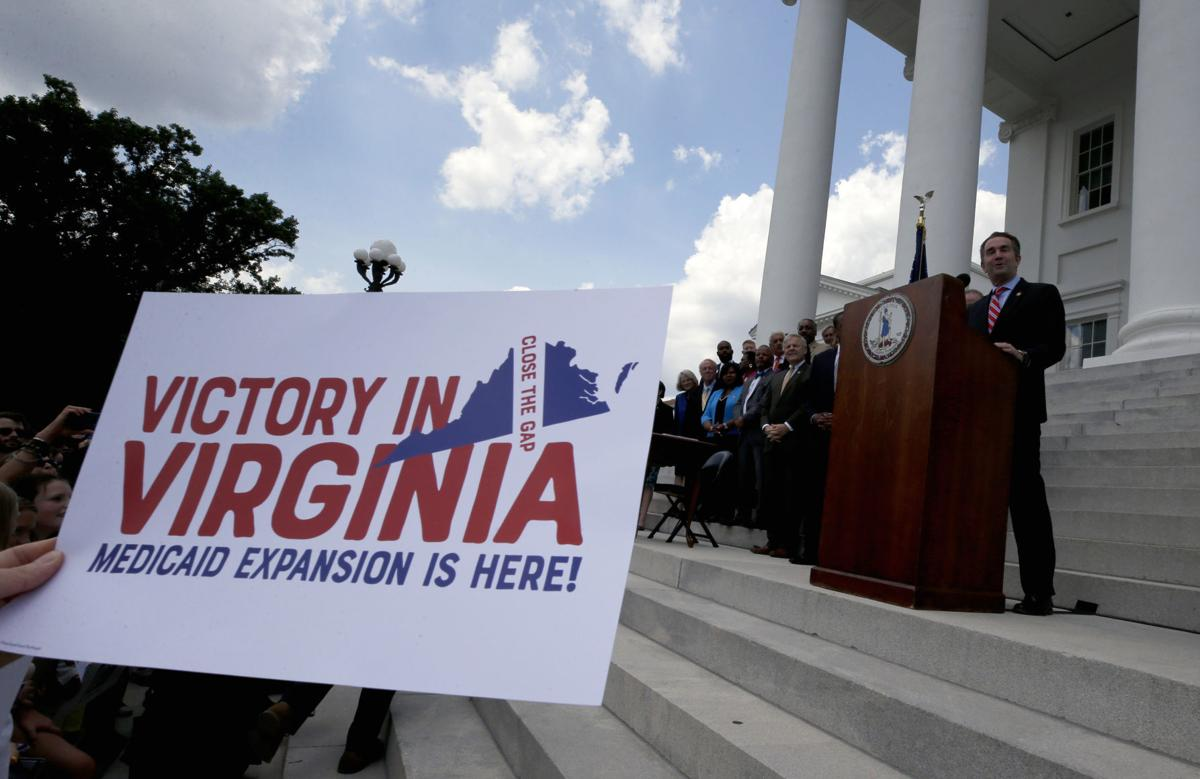
\includegraphics[width=0.99\linewidth]{Plots/Web/va_medicaid_expansion} \caption{Medicaid Expansion in Virginia}\label{fig:medicaid-expansion-va}
\end{figure}

\hypertarget{montana}{%
\subsubsection{Montana}\label{montana}}

\begin{figure}
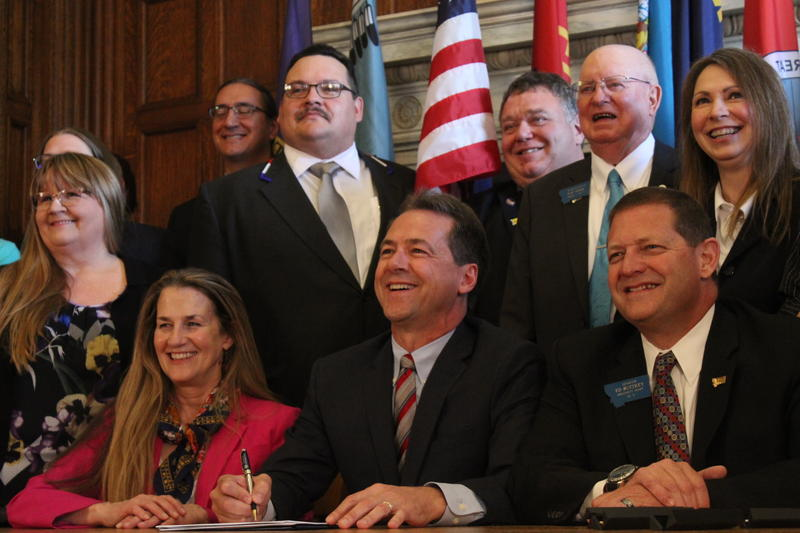
\includegraphics[width=0.99\linewidth]{Plots/Web/mt_medicaid_expansion} \caption{Medicaid Expansion in Montana}\label{fig:medicaid-expansion-mt}
\end{figure}

\hypertarget{overall}{%
\subsubsection{Overall}\label{overall}}

The overall picture in the country in Figure \ref{fig:medicaid-expansion-map} shows Medicaid expansion happened in a large majority of states as of December 2020. However, big holdouts like Texas and Florida continue under the pre-2010 system of extremely tight eligibility for Medicaid.

\begin{figure}
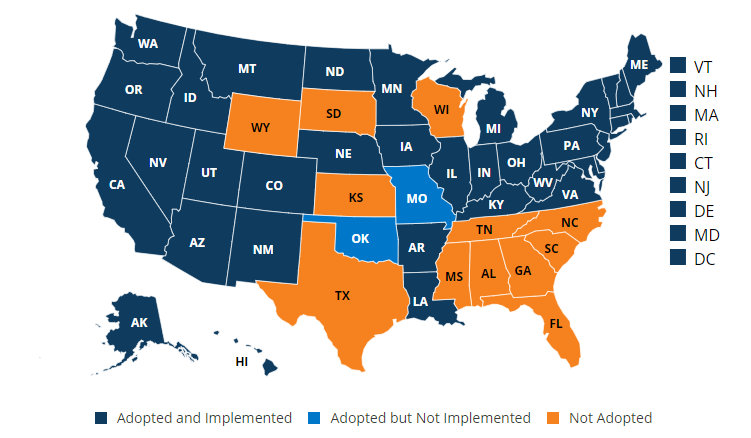
\includegraphics[width=0.99\linewidth]{Plots/Web/medicaid_expansion_map_2020} \caption{Medicaid Expansion in the States as of December 2020}\label{fig:medicaid-expansion-map}
\end{figure}

\hypertarget{the-public-option-in-washington-state}{%
\subsection{The Public Option in Washington State}\label{the-public-option-in-washington-state}}

President Biden was elected after having promised a public option as a prominent part of his 2020 electoral campaign. As of this writing, the public option appears to have been put on the backburner, behind the push for stimulus, infrastructure, and family omnibus spending bills. The president has instead used executive orders to, amongst other things, reopen the signups for exchange marketplaces.

Legislative action on the public option instead actually exists in Washington State. There, Eileen Cody wrote a bill that was eventually passed in the legislature and signed by Governor Inslee.

\begin{figure}

\includegraphics[width=0.5\linewidth]{Plots/Web/eileen_cody} 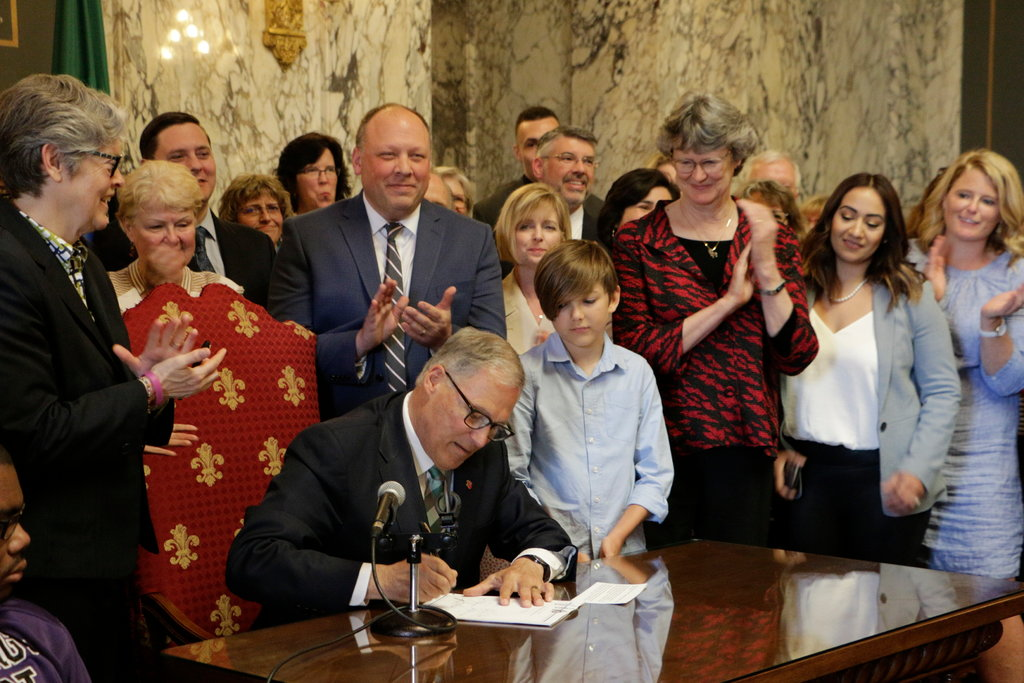
\includegraphics[width=0.5\linewidth]{Plots/Web/washington_public_option} \caption{The Public Option in Washington State. Eileen Cody, bill author, and signing ceremony}\label{fig:wastate-publicoption}
\end{figure}

\hypertarget{single-payer-in-california}{%
\subsection{Single Payer in California}\label{single-payer-in-california}}

In California, a single payer bill (SB 562) that would have utilized a section 1332 innovation waiver--pushed by progressive Democrats and the state nurses union--was adopted by the California State Senate in June 2017. Yet shortly thereafter, the Democratic Speaker of the Assembly decided to table the legislation, to the fury of its supporters. The state is marked by unified Democratic control of the legislature and the governorship, so a simple partisan analysis of why SB 562 failed would fail to provide insight. The internal fight in the Democratic party to push a state response to Trump administration policies is the centerpiece of trying to understand the future of Affordable Care Act in the nation's largest state. That fight is still ongoing, as 16 bills have just been introduced by Democrats in July 2018, including another attempt at single payer.

The Virginia and California stories are microcosms of what is happening across the country's over 7,000 individual state legislative districts. While state capitols are the site of much of the action, so too is the district-by-district contest to push for health policy changes. Similarly, while \emph{interparty} dynamics between Republicans and Democrats are important, yet many of the policy reforms are being hashed out in the context of \emph{intraparty} debates and single-party states. Yet we know very little about how policy is developed at the district and intraparty levels. This project would aim to change that.

\hypertarget{downs-syndrome-coverage-in-montana}{%
\section{Downs syndrome coverage in Montana}\label{downs-syndrome-coverage-in-montana}}

\begin{itemize}
\tightlist
\item
  H 318 requires insurance to cover the diagnosis and treatment of minors with Down's syndrome

  \begin{itemize}
  \tightlist
  \item
    104 sessions/year with speech pathologist, and 52 sessions/year with physical therapist \& occupational therapist
  \item
    Sponsored by Ellie Hill (D), most liberal 10\% of chamber, 27\% of Ds
  \end{itemize}
\item
  Senate R majority gets rolled, House R majority divided

  \begin{itemize}
  \tightlist
  \item
    76-23 final vote in House (41-0 D, 35-23 R)
  \item
    56-40 final vote in Senate (40-0 D, 16-40 R)
  \item
    Signed by Governor Bullock (D)
  \end{itemize}
\end{itemize}

\begin{figure}

{\centering 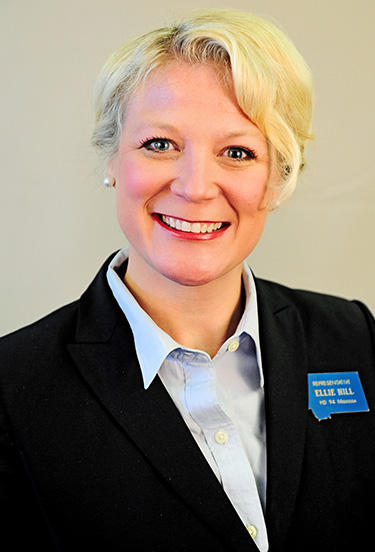
\includegraphics[width=0.33\linewidth]{Plots/Web/ellie-hill-mtleg} 

}

\caption{Montana Representative Ellie Hill}\label{fig:intro-elliehill}
\end{figure}

\hypertarget{surprising-billing-regulation}{%
\section{Surprising Billing Regulation}\label{surprising-billing-regulation}}

Balance bills are colloquially called ``surprise bills.'' They generally occur when insured individuals receive emergency care at an out-of-network facility or from an out-of-network provider, or when they receive elective nonemergency care at an in-network facility but is inadvertently treated by an out-of-network health care provider. Being out-of-network is crucial since insurers typically refuse to pay a large portion of these bills. In turn, then, the provider or facility might bill the insured individual, who is surprised to find a huge bill due despite their insurance coverage.

While surprise billing restrictions were enacted by Congressin December 2020 -- and only comes into effect in 2022-- states had for years enacted these protections. Even Texas--whose legislature only meets for six months every two years--passed this bill before Congress finally moved.

\begin{figure}
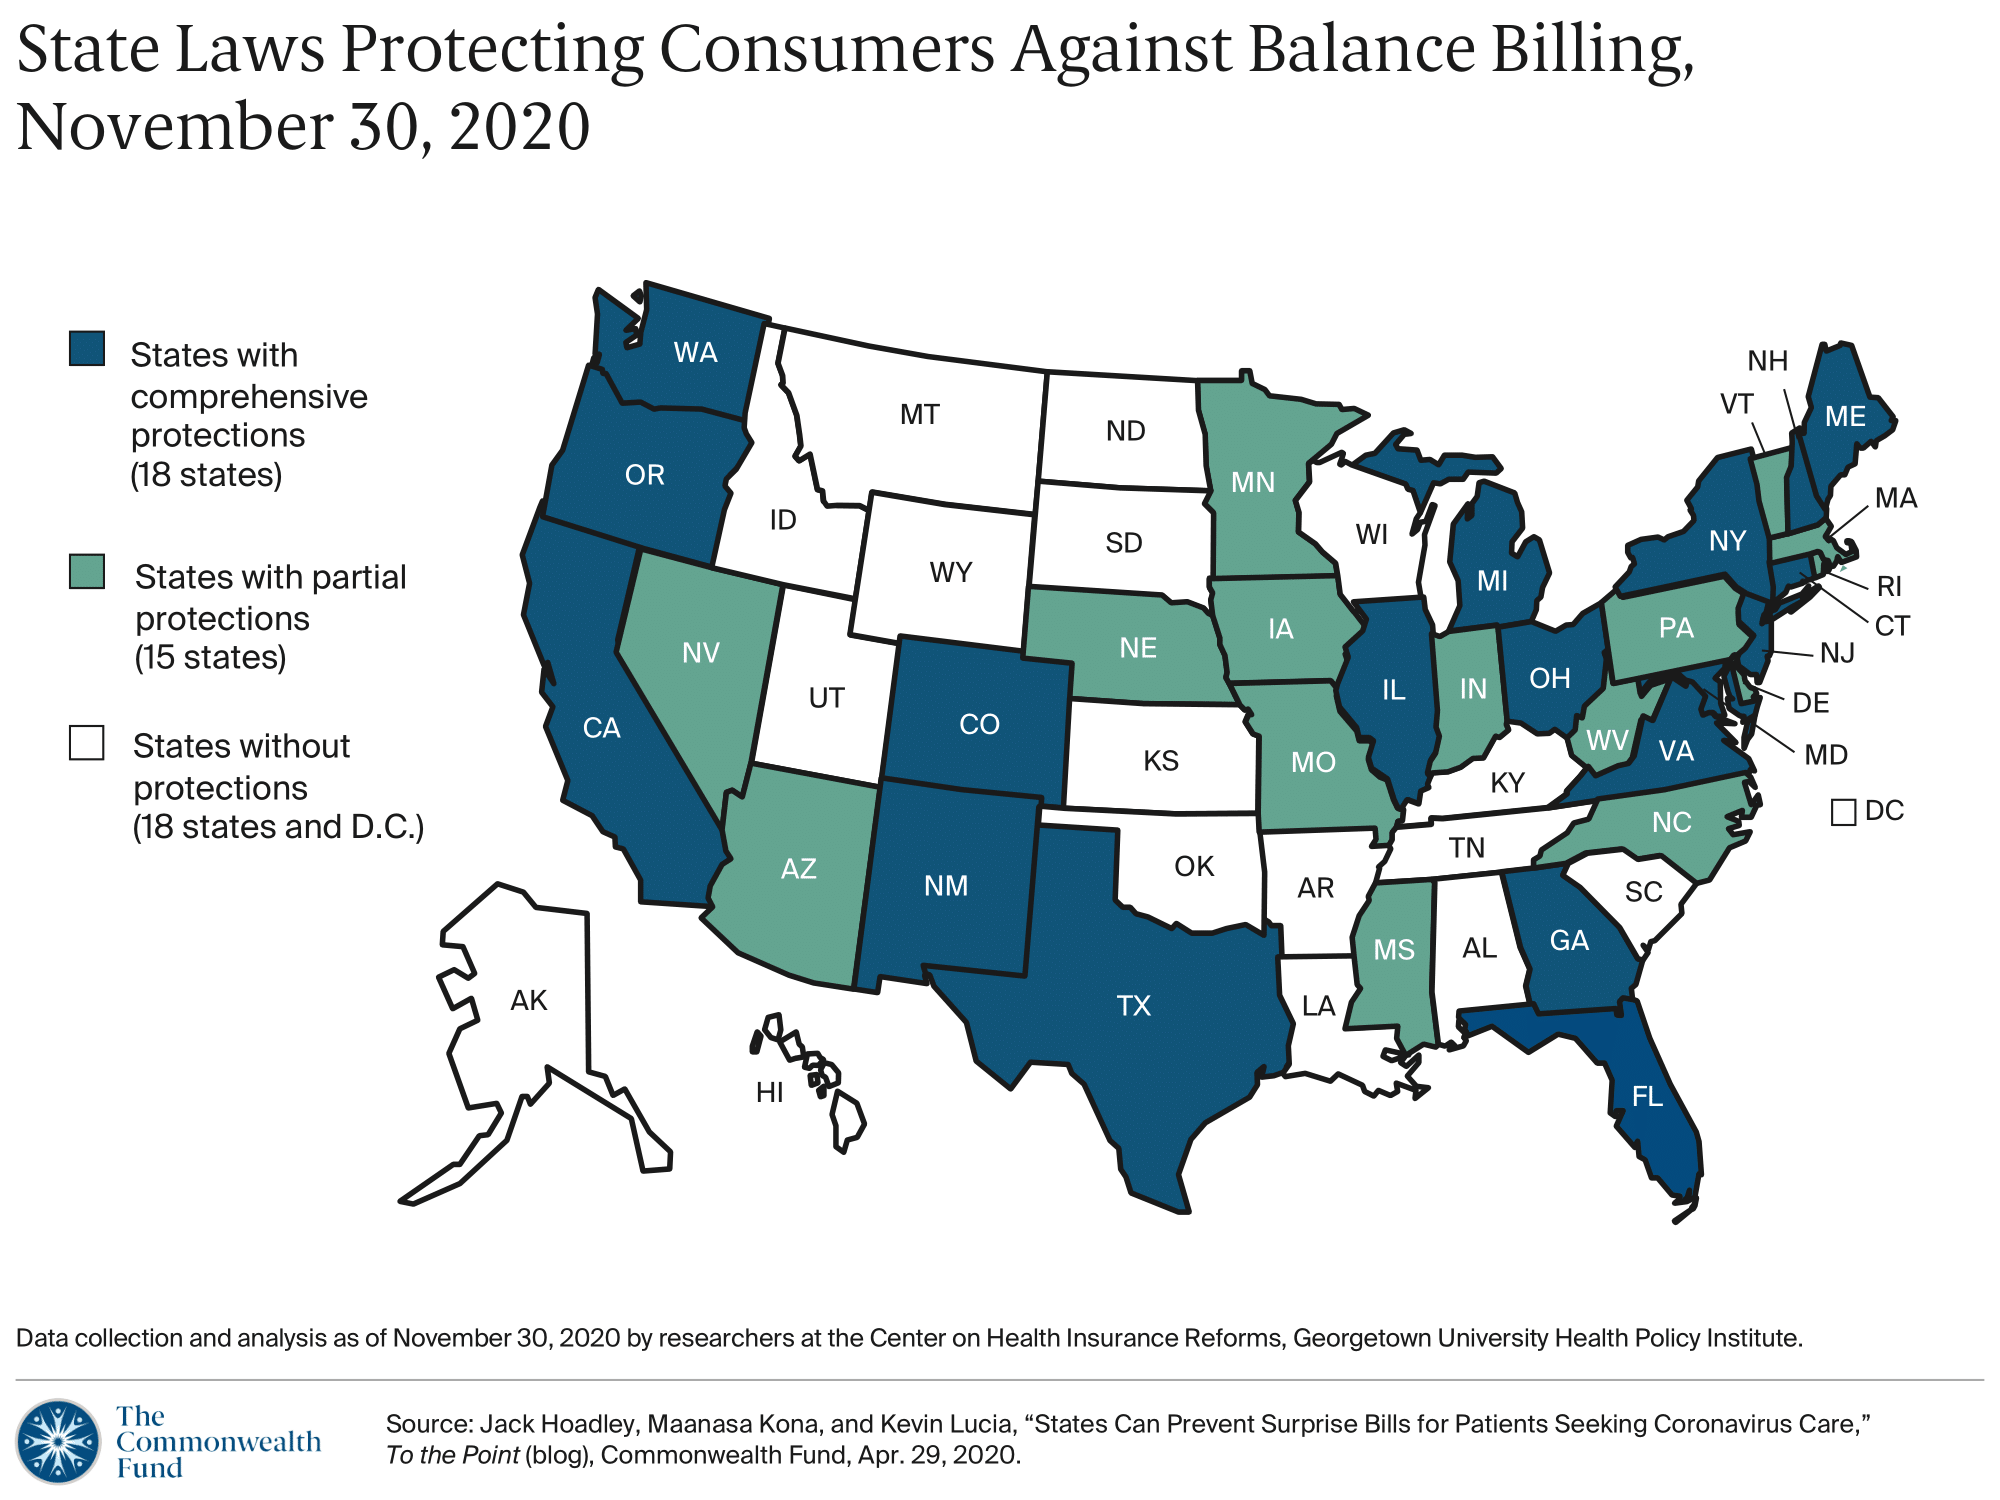
\includegraphics[width=0.99\linewidth]{Plots/Web/state_balance_billing_map_feb21} \caption{Balance Billing State Laws, November 2020}\label{fig:surprise-us}
\end{figure}

\hypertarget{autism-coverage-mandates}{%
\subsection{Autism coverage mandates}\label{autism-coverage-mandates}}

Two decades ago, insurance companies only covered the extensive therapy required by autism-spectrum patients idiosyncratically. That changed over the 2000s, and by 2019 the final state, Tennessee, passed the 50th autism insurance mandate in the country.

\begin{figure}
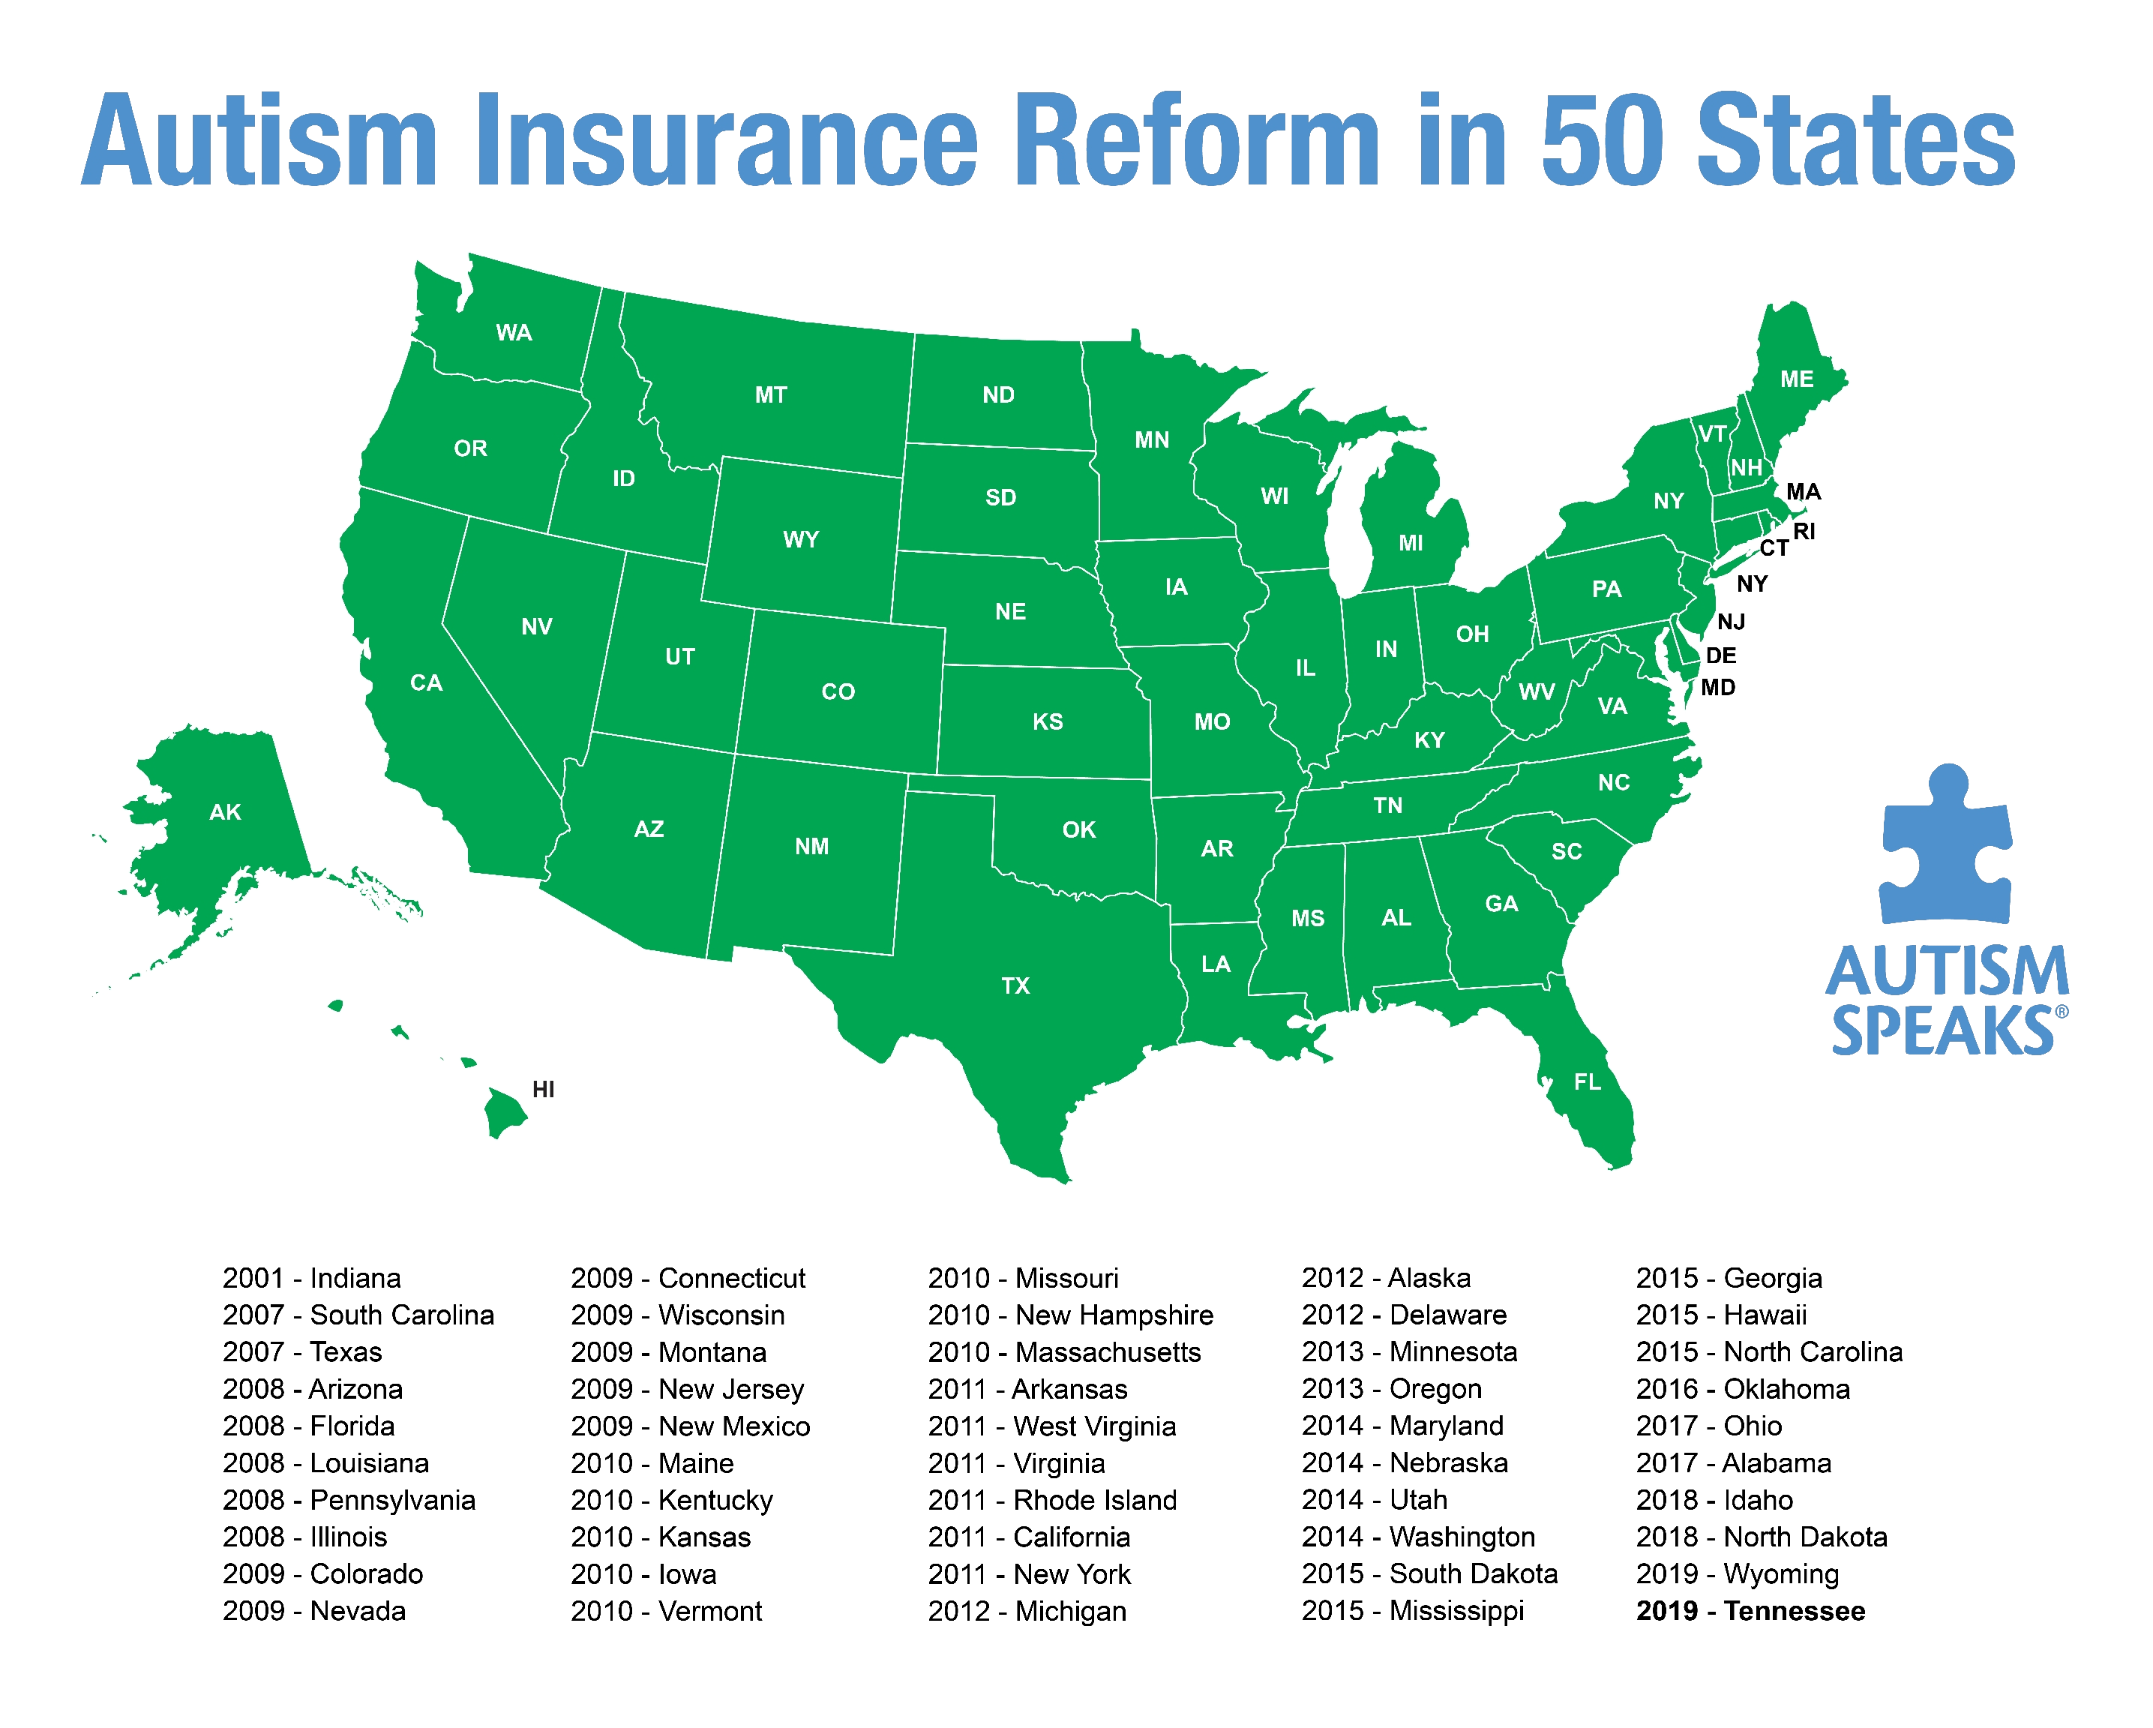
\includegraphics[width=0.99\linewidth]{Plots/Web/autism_coverage_map} \caption{Autism coverage mandates in the states}\label{fig:autism-map}
\end{figure}

\hypertarget{covid-response}{%
\subsection{Covid Response}\label{covid-response}}

\begin{figure}
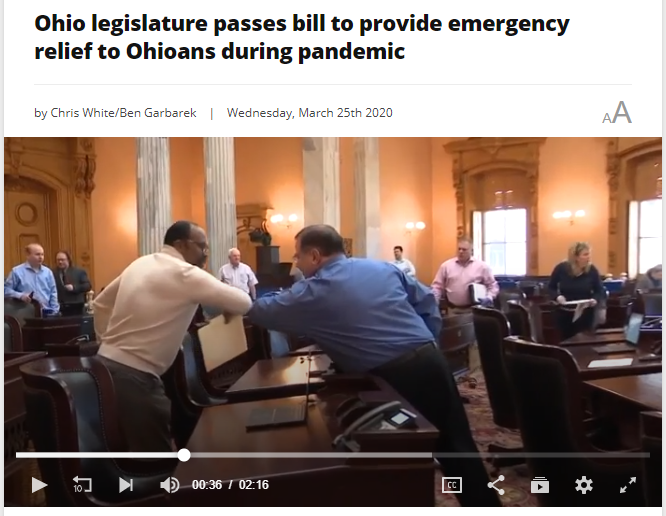
\includegraphics[width=0.99\linewidth]{Plots/Web/oh_legislature_covid_hb197} \caption{Early Days of Bipartisanship during the Pandemic}\label{fig:covid-oh}
\end{figure}

\hypertarget{the-bigger-picture}{%
\section{The bigger picture}\label{the-bigger-picture}}

How well do the unsung workhorses of American representative democracy--its thousands of state legislators--represent their constituents on the most vital issues of the day? Are the decisions they make in the statehouse reflective of the wishes and needs of their constituents, or do other influences--their own preferences, those of their party, and those of particularized interests--hold more sway? This question is particularly important in understanding the thoroughly politicized domain of health care. Policy made in statehouses affects the lives of hundreds of millions of Americans, yet little is known about how that representational relationship actually works. The project proposed here will advance our understanding of these relationships, specifically by the use and amalgamation of new sources of data that would have been impossible only a few years ago.

I identify five relevant influences on state legislators in their bill introductions, sponsorship, committee action, and roll call voting behavior. Do more liberal views by district constituents on the Affordable Care Act predict more liberal voting patterns by their representatives in the statehouse? Do objective measures of need -- specifically measures of poverty and health insurance coverage -- also predict such patterns? Or are such variables overridden by legislators' own ideological preferences or partisanship? What role do particularized interests--both of the ideological and economic interest varieties--play in influencing legislators?

Whether elected representatives' behavior is congruent with constituent opinion and policy needs is a fundamental inquiry in a representative democracy, and has been a major touchstone in the research on American politics. However, earlier work concentrates on representation at the federal level. When states are studied, it is almost entirely in statewide terms. Finally, representation is understood in general ideological terms rather than in specific policy areas like health. In short, we know very little what happens in the states, in terms of specific policies, and at the district level because of measurement difficulties. This project would address those issues by the use of new data and new techniques. Bringing these together would allow us to understand how and when viable coalitions to implement (and delay) Affordable Care Act implementation in the states.

\hypertarget{early-findings-from-this-study}{%
\subsection{Early Findings from this study}\label{early-findings-from-this-study}}

\begin{itemize}
\tightlist
\item
  Health reform in the states is moving leftward in legislatures. Why?
\item
  Democratic majority chambers

  \begin{itemize}
  \tightlist
  \item
    Disproportionate production of health care legislation
  \item
    Agenda control is strong
  \item
    Party is united
  \item
    Liberal proposals dominate and succeed relative to moderate and conservative ones
  \end{itemize}
\item
  Republicans majority chambers
  - Substantial failures of agenda control- Substantial failures of party discipline in voting
  - Moderate bills do very well, liberal bills often succeed
\end{itemize}

\hypertarget{why-study-states}{%
\subsection{Why study states?}\label{why-study-states}}

The explicit federalist design of the Constitution, as well the specific institutional history and context of American health policy making, means that states have a major role to play in how the Affordable Care Act unfolds in the post-2016 political environment. Indeed, placing states at the center of ACA implementation was meant to ameliorate political opposition to the ACA, both within the Democratic party (to appease moderates like Nebraska Senator Nelson), and as a way to reach out to Republicans.

In short, states are where the policymaking action is, as long as Congress remains mostly gridlocked when it comes to health. The National Conference of State Legislatures counts 111 enacted state bills in 33 states since January 2017 alone that directly address specific choices states have under the ACA.\footnote{Taken from the NCSL Health Innovations Database, July 2018. See \url{http://www.ncsl.org/research/health/health-innovations-database.aspx}} Alaska, Kentucky, Maine, Texas, New Hampshire, and Oklahoma all enacted legislation authorizing applications for section 1332 innovation waivers (sometimes called ``superwaivers'\,'). These are nearly all Republican-controlled states, and these waivers can be expected to undermine the ACA at the state level, especially given the signaled support from the Trump Administration to grant these waivers. Other, typically Democratic, states like California, Hawaii, Nevada, and Minnesota has passed laws which augment the ACA's provisions for their populations. Reinsurance programs have been approved via 1332 waivers in Minnesota, Alaska, Oregon, and New Jersey. In New Jersey, too, a newly elected Democratic governor signed a state health insurance mandate bill to counter the national law eliminating the mandate (so too did a Republican governor in Vermont). All in all these are themselves only a portion of all health insurance reforms that indirectly touch on the ACA: 639 laws in all 50 states in 2017-2018 alone, and more than 1,400 laws passed since 2015.

The important political context is the partisan division of state control. After the 2016 and 2017 elections, Republicans now have unified control of 32 state legislatures (25 states with ``trifectas'\,' of unified control of both chambers and the governorship). Yet Democrats, too, control state legislatures in 14 states (8 states with trifectas) -- far fewer, but including large states like California and New York. The Blue Wave propelling Democrats to victories in the 2018 midterm elections are also likely to be mirrored at the state level, since research shows these to be highly correlated \citep{Rogers:2016}.

Now that the congressional battle is over, and state policies challenging (and augmenting) the ACA are accelerating, the question naturally arises whether state policy, too, will override public opinion. This is crucial because the ACA gives tremendous discretion to states to modify policy implementation on the ground, and the presidency gets nearly unlimited scope to approve these modifications, especially waivers. Will, for example, section 1332 waivers undermining (and augmenting) the ACA pass despite public approval for the ACA as a whole?

Another puzzle that needs unraveling is the disjuncture between health policy lawmaking at the state versus national levels. Health policy is often severely gridlocked at the national level. Even beyond the gridlock induced by multiple veto players \citep{Krehbiel:1998}, health policy in particular is far more gridlocked than other policy types \citep{Volden:2011}. Yet at the state level, this is far less true, and this difference is not new. Major health reforms have been implemented in many states that have not moved at all at the national level \citep{Gray:2013}.

In terms of state health policy, there is a tremendous amount of lawmaking going on, even in controversial areas. Since 2015, several hundred health reforms laws have been enacted with over 1,000 final passage roll call votes. Strong supermajorities of Democratic support for the reforms is not surprising. Yet far from unanimity in opposition, Republicans at the state level have voted for these reforms at strikingly high rates, at nearly 50\%. Even the most controversial reforms attract significant Republican support, such as Medicaid expansion (20\% support) and state health insurance exchanges (28\%). These Republican votes have often provided pivotal in the passage of these reforms. The evidence for Republican support for a much wider array of health policy reforms is quite striking. Figure @ref(topic.splits) shows the split of the parties on final passage votes for 15 of the most common health policy reforms. Democrats vote at high rates, but Republicans do sometimes, too. Bipartisan coalitions frequently roll majority parties in the states at rates unheard of in Congress.

A broader preliminary look at far more health policies (see below) shows that the Republican party is deeply divided in its votes for health reform measures (see \textbf{Figures x-y}). On average, the party votes in favor of such measures at around 50\%, a figure that masks incredible variation at the state, topic, and ideological level. Understanding when and why Republican votes on progressive policy reforms can be forthcoming is crucial to mapping out the future of ACA implementation in the states. In the fight to expand Medicaid, knowing which concessions in which states need to be made can help in constructing progressive policy coalitions.

At the same time, while the Democratic party has been much more homogenous in its support for standard progressive health reforms, bleeding edge innovations like single-payer have been much more internally divisive. Especially in Democratic-dominated states like California, attention to the intraparty debate is much more insightful than examining the state interparty divide in a place where the Republican party is almost totally irrelevant.

\hypertarget{why-study-districts}{%
\subsection{Why study districts?}\label{why-study-districts}}

Since lawmaking involves the construction of a series of majoritarian and supermajoritarian coalitions in the state legislatures, understanding legislator-level decisions in that process is crucial. Legislators choose on their own whether to sponsor a bill, whether to propose an amendment, and how to vote on an endless stream of roll calls. They make these decisions under the eye of legislative party leaders and the governor, not to mention the news media, donors, interest groups, and their constituency, but the decision is an individual one.

This is well understood in studies of Congress, where individual legislator decisions contraposed with district level factors is fairly common. But for states, macro-representation dominates. Aggregate outcomes across states and times are compared with dynamic state-level factors. Since policy is the output of a complex set of state level institutions, this is an entirely appropriate level of inquiry. But it does not supplant the need to understand individual legislator behavior, particularly in understanding when and where coalitions form to pass particular policies.

A major reason for the imbalance in favor of studies of macrorepresentation is the incredible difficulties of measurement in district or legislator-level microrepresentation (as contrasted with Congress). Yet a methodological and measurement revolution has generated groundbreaking new measures and techniques which is changing all of that. Whereas measures of simple partisanship were all we had only a few years ago, now we have legislator-level ideal point measures for the past two to three decades \citep{Shor:2011, Shor:2020}. Whereas we had only district-level demographic information as proxies for opinion, now we have district-level measures of general ideology \citep{Tausanovitch:2013}, and techniques to get district-level opinion on specific policies {[}\citet{Warshaw:2012}; Shor:2018{]}. District-level measures of interests were impossible before, while now we can get donor-level data aggregated to the district level \citep{Bonica:2013, Bonica:2017, Bonica:2017a}. Bill and roll call information, too, was locked in legislator journals and other inaccessible sources. Changes by states themselves and open government initiatives like OpenStates has made these now fully searchable and accessible electronically.

\hypertarget{literature}{%
\chapter{Literature}\label{literature}}

Two major perspectives, attributed to Edmund Burke, purport to define the essential nature of representation in a democracy for legislators: delegates, who are supposed to mirror constituents' opinions, and trustees, who are supposed to be introspective when it comes to delivering what is best for their constituents. Beyond normative concerns, which actually describes legislator behavior empirically? The literature has focused on areas where measurement is easier: on Congress, on states as a whole, and on generalized representation via responsiveness. We know very little about how well representation works on important, specific policies like health reform, and we know even less about dyadic representation at the legislator/district level.

\hypertarget{delegative-representation}{%
\section{Delegative Representation}\label{delegative-representation}}

Most of the work on this kind of representation has focused on Congress. The logic of the connection starts with \citet{Mayhew:1974} who argued the linchpin of legislator accountability is their concern for re-election. Yet empirical support for the strength of the electoral connection has been limited to more general voting behavior \citep{Canes-Wrone:2002}, as opposed to votes on specific issues where legislators appear to have lots of freedom to maneuver. \citet{Poole:2007a} finds little evidence that constituency need is a major determinant of legislator votes. One interesting counterexample is {[}\citet{Nyhan:2012} which found that moderate Democrats voting in favor of the then-unpopular ACA suffered substantial losses at the polls, and maybe even enough to help flip Congress to Republican control in 2010.

Even at the congressional level, studies of representation have been hampered by the difficulty of measuring public opinion at the district level. Most studies proxy for district ideology using presidential vote \citep{Levendusky:2008, Kernell:2009}. More modern measures employ newer statistical estimators to model district opinion \citep{Tausanovitch:2013, ShorKousserPhillips:2016}, but these applications were with generalized measures of district ideology and not responses to specific issues.

What about the state level? States are much more likely to be dominated by a single party, and information on activity in state capitols is very poor, especially given the near-destruction of traditional newspaper state political coverage. Compounding the lack of information is the nationalization of state elections in recent years. National factors like presidential popularity and generic party approval have increasingly dominated state factors \citep{Hopkins:2018}. This raises the concern about how well the electoral connection can work at the state level if constituents vote on national rather than state level issues.

Most work has been done on responsiveness of generalized policy outputs, aggregating over all the different policies that states produce, with general findings of responsiveness \citep{Erikson:1993, Caughey:2017}. Less work has focused on state representation at the policy level, but the major findings suggest responsiveness but relatively little congruence \citep{Lax:2009, Lax:2009b}.

More to the point, very little is known about the influence of constituents on their state legislators. What little we know suggests a limited role for the public in legislator decisions. State legislative elections are very uncompetitive. In 2016, about 42\% of general election contests and 79\% of primary election contests were uncontested even nominally: that is, only a single name appeared on the ballot. Incumbents that do face opponents rarely lose (except in wave elections like 2014). At the same time, the public is barely aware of which party controls the state legislature in general, much less the name of their own representative, and legislators lose very little when they are out of step of their districts in general \citep{Rogers:2017}.

As with Congress, the difficulties of measurement plague district level studies of representation. We presidential vote by legislative district, data only available for 2012 and 2016 via crowdsourcing by the Daily Kos. Generalized ideology measures from {[}\citet{Tausanovitch:2013} are also available, but these aggregate over an entire decade and do not address individual policies. Finally, state legislators themselves have consistently inaccurate images of public opinion in their own district \citep{Broockman:2017}. They are nearly as blind as their constituents.

\hypertarget{trustee-representation}{%
\section{Trustee Representation}\label{trustee-representation}}

As with delegative representation, nearly all the work on trustee-type representation at the legislator level have been done in the congressional context. There, the contrast with the ``trustee'\,' variables of partisanship, ideology, and interests at the legislator level could not be more striking. Party \citep{Lee:2009, Lee:2016} and ideology \citep{Poole:2007a} are the strongest known influences on congressional behavior. The parties are polarizing rapidly \citep{Barber:2015} and the same district can elect a Democrat or a Republican and experience vast differences in representation \citep{McCarty:2009}.

State level work on representation in the health policy area almost always cites partisanship as the most important predictor of progress in ACA implementation \citep{Rigby:2013, Jacobs:2013, Jones:2014, Barrilleaux:2014, Haeder:2015, Callaghan:2016, Callaghan:2017}. Ideological divisions within state Republican parties between a more extreme Tea party faction and a more moderate business-oriented faction has been cited as explaining variation in expanding Medicaid \citep{Hertel-Fernandez:2016}.

What we know about the influence of party and ideology on specific policy outputs at the state legislator level is relatively limited. In general terms, state legislative parties are polarizing \citep{Shor:2011, Shor:2020}. Moderate, heterogeneous districts elect extreme Republicans and Democrats \citep{Rodden:2018} In terms of specific policy, my own work addresses this on a small set of health policies and roll call votes \citep{Shor:2018}.

\hypertarget{interest-representation}{%
\section{Interest Representation}\label{interest-representation}}

Interest groups are an important part of the American political system and their influence is well know to operate through campaign finance and especially lobbying channels \citep{Hall:1990, Evans:1996}. Campaign finance is now a much more important channel, especially in the states, because of the \emph{Citizens United} decision and many state laws which essentially have no limits on donations.

State health policy has long attracted the attention of scholars interested in illuminating the role of interests in the policymaking process \citep{Lowery:2008, Gray:2013}. A newer literature focusing on the implementation of the Affordable Care Act at the state level continues this tradition. For example, \citet{Callaghan:2016} document the influence of business interests in retarding ACA implementation, and public interest advocates in pushing it forward. \citet{Rose:2015} cites the role of resource-starved hospitals in particular on Medicaid expansion. Yet these influences can not be measured at the individual level. Bill-level measures give us more detail, like those in \citet{Garlick:2016} who finds that business lobbying pressure moderates polarization on individual bills while public interest advocacy amplifies it.

States are also the site for the unmatched influence of the conservative Koch network groups: the American Legislative Exchange Council, Americans for Prosperity, and the State Policy Network. These work together to provide expertise and resources to the resource-starved efforts of mostly amateur and part-time legislators. These three organizations have built an infrastructure over decades, and not at all matched by the disjointed, less comprehensive, and far more nascent efforts on the left \citep{Hertel-Fernandez:2016a}. These operate explicitly at the legislator level, providing model bills and other resources directly to individual members, especially backbenchers without institutional resources \citep{Hertel-Fernandez:2014}.

Physicians have a very special role in the setting of health policy. More than any other group, they are trusted by members of the public when it comes to making health policy choices \citep{Patashnik:2017}. Yet physicians have long had a strong professional and ideological bias against health reform that has doomed previous reforms over American history \citep{Starr:2008, Starr:2013}. At the same time as possessing the public's trust, physicians are educated, wealthy, geographically dispersed, and unusually politically active \citep{Bonica:2017a}.

But what do physicians believe? New measures have been introduced directly measuring the ideology of physicians based on party registration \citep{Bonica:2014, Bonica:2015} and campaign finance donations \citep{Bonica:2017, Bonica:2017a}. These attest to the vast geographic heterogeneity in physician policy preferences. While new studies find geographic sorting by ideology is limited \citep{Mummolo:2017}, this does not appear to be the case for physicians given their incomes and their ability to find work across the country (and the quasi-randomization induced by the residential matching program after medical school) \citep{Bonica:2017a}. Physicians have sorted into distinct geographic areas (within and across states), and this naturally raises the possibility that this sorting has political and policy consequences.

\hypertarget{issue-ownership}{%
\section{Issue Ownership}\label{issue-ownership}}

Not all issues are the same. Pioneering work by \citet{Petrocik:1996}; \citet{Petrocik:2003} and others have shown how one or the other major parties have advantages over certain issues in the eyes of the public. The public perceives that the parties prioritize certain issues over others, and these priorities are enduring over time \citep{Pope:2009, Egan:2013}. The connection to representation is that parties are \emph{less} responsive on issues they own than on those they don't. Health as a category is considered owned by Democrats so this should imply that Republicans are actually more responsive to public opinion on this issue.

The issue ownership literature has not investigated spatial heterogeneity in issue ownership, partly because the focus has been exclusively on national politics. It may be that Democrats own health care in some states, but not all. Voters in South Carolina or Utah might see Republicans as owning the issue, especially as Democrats are nowhere near the policymaking reins in either state. Furthermore, it could be the case that ``health'\,' is simply too big a catchall category to adequately describe voters' opinion. Perhaps Republicans own tort reform in the very same state that Democrats own Medicaid expansion or prescription drug pricing.

\hypertarget{theory}{%
\chapter{Theory}\label{theory}}

The major hypotheses I investigate is whether, which, and to what degree partisanship, ideology, and interests outweigh and/or condition the effect of constituency opinion and needs when explaining legislator behavior. The primary mechanism assumed to be driving responsiveness is the electoral connection. When that electoral connection is tighter--for example, when issues become more salient--legislators should be more responsiveness. When the electoral connection is looser--for example, when knowledge of statehouse activity by constituents is absent--legislators should be less responsive to their constituents, and more affected by interests or their own characteristics like ideology. Heterogeneity in these effects will also be considered, as detailed below.

\hypertarget{heterogeneity-by-legislator-party}{%
\section{Heterogeneity by Legislator Party}\label{heterogeneity-by-legislator-party}}

Do Republican and Democratic legislatures represent their constituents in symmetric fashion? If so, the image of the parties as equally extreme relative to a moderate public and trading off ``leapfrog representation'\,' \citep{Herron:2010} may not be correct. Most scholars using national evidence argue that the Republican party is not a mirror image of the Democratic party, and is much more prone to extremism \citep[Mann:2016]{Hacker:2015}. The quantitative evidence for this conclusion comes from studies of elites and public partisans. For example, \citet{McCarty:2013} cite NOMINATE scores to show that Congressional Republicans appear to be polarizing faster than Democrats, and \citet{Grossmann:2016} critically examine the internal activist coalitions that make Republicans more ideologically oriented than Democrats. \citet{Ellis:2009}, Ellis:2012 show that Republicans have an advantage in representing the public's symbolic conservatism which nevertheless conflicts with their weakness in representing their more substantive issue-based liberalism. \citet{Lelkes:2016} cites the greater ideological awareness by Republican partisans as a source of the party's ability to resist positions broadly popular with the public as a whole.

But this evidence is overwhelmingly at the national level. Partisan asymmetry in representation is very much an open empirical question. \citet{Shor:2020} complicates the picture by showing heterogeneity of asymmetry geographically for state legislatures, with Democrats polarizing faster in the South and West, and Republicans in the Midwest and Northeast. \citet{Lax:2012} find that states controlled by both parties overshoot the moderate public in roughly symmetric fashion.

At the legislator level, \citet{Broockman:2017} shows evidence that state legislators systematically misperceive the opinion of their districts (measured with district-level MRP). A party asymmetry exists in that Republicans misperceive district conservatism more than Democrats, a difference partly driven by the greater political activism of district Republicans in contacting and lobbying the legislators. If true, we should expect to see lower responsiveness and congruence by Republicans than by Democrats, something that I will test.

\hypertarget{heterogeneity-by-constituent-knowledge}{%
\section{Heterogeneity by Constituent Knowledge}\label{heterogeneity-by-constituent-knowledge}}

Do the heterogenous presence of informational resources (like state capitol reporters) do so as well?

\hypertarget{heterogeneity-by-salience}{%
\section{Heterogeneity by Salience}\label{heterogeneity-by-salience}}

Does policy salience amplify constituency influence? \citet{Lax:2009}, Lax:2012 show that state policy on more salient issues like abortion and same-sex marriage is more responsive than those on less salient issues. Similarly, legislators should feel more pressured to follow district opinion on policies where there is more information.

Health policy, especially components of ACA implementation like Medicaid expansion, is a similarly fairly salient policy in general \citep[Pacheco:2016]{Pacheco:2011}. Nevertheless, within health policy, there are big differences in information that could be relevant. Medicaid expansion or work requirements is likely to be highly salient, and our expectations would be for higher responsiveness and congruence in that policy area. Medicaid payment reforms, provider network requirements, or electronic medical records implementation are far more technical and hidden, and likely to activate particularized interests far more than public opinion. The disaggregation of the policy topics will be crucial to test this causal pathway (see below).

\hypertarget{heterogeneity-by-electoral-environment}{%
\section{Heterogeneity by Electoral Environment}\label{heterogeneity-by-electoral-environment}}

In a second paper, I aim to see the degree to which legislator votes on especially salient issues affect the electoral fortunes of state legislative candidates, as they did to some degree in Congress in 2010 \citep{Nyhan:2012}. No such study exists at the state legislative levels. If evidence of such electoral effects exists, then some predictions can be made as to the outer constraints on legislator votes undermining the ACA at the state level.

The constituency to whom legislators are responsive has long been a topic of interest to scholars \citep{Fenno:1978}. Is it the primary election constituency \citep{Brady:2007a, Hall:2013, Hall:2015} or the general election constituency \citep{Canes-Wrone:2002, Ansolabehere:2001}? All extant research focuses on Congress, and I aim to extend that to the state legislative context. I will conduct two surveys and ask questions around the time of the primary as well as the general election to try to tease out the information that constituents might have regarding their candidates.

\hypertarget{heterogeneity-by-state-variation-in-issue-ownership}{%
\section{Heterogeneity by State Variation in Issue Ownership}\label{heterogeneity-by-state-variation-in-issue-ownership}}

Scholars have found that health care is an issue owned by Democrats {[}\citet{Petrocik:1996}; Petrocik:2003; Egan:2013{]}, which is to say that voters identify Democrats as the party that overwhelmingly prioritizes health care. Yet the evidence for this finding comes exclusively from national survey data. I will investigate the degree to which issue ownership varies by state, since in many states single party domination might amplify the reputation of the ruling party and the undermine or muddy the reputation of the dominated party. If true, this should condition the relationship between issue ownership and responsiveness and strongly qualify the \citet{Egan:2013} finding that congressional responsiveness is moderated by issue ownership.

\hypertarget{heterogeneity-by-institutional-difference}{%
\section{Heterogeneity by Institutional Difference}\label{heterogeneity-by-institutional-difference}}

\citet{Lax:2009}; \citet{Lax:2012} and \citet{Lewis:2017} show that institutional differences across states, specifically varying degrees of professionalization and the presence of direct democracy, affects the representational relationship between state opinion and state policy. I can see whether these findings hold at the microlevel. One such difference are campaign finance rules. In 2010, the \emph{Citizens United} Supreme Court decision struck down restrictions on independent expenditures during election campaigns for both federal and state elections. In some states, these restrictions did not exist, while they did in others. The difference-in-differences estimate for this change can be interpreted to explicate how much less representative are legislator decisions when unrestricted campaign expenditures are allowed when they used to be restricted. Another such decision is \emph{Janus v. AFSCME} (June 2018) which will make it much harder for public sector unions in many states to engage in political activity \citep{Feigenbaum:2018}. But since a number of states already restricted these unions in similar ways (for example, Wisconsin), we can take advantage of the natural experiment afforded by the exogenous shock of the decision to compare the differences in the trends of the \texttt{treated\textquotesingle{}\textquotesingle{}\ states\ (those\ whose\ unions\ were\ legally\ unobstructed)\ to\ those\ of\ the}control'\,' states (those whose unions were legally bound).

\hypertarget{heterogeneity-by-interest-types}{%
\section{Heterogeneity by Interest Types}\label{heterogeneity-by-interest-types}}

\citet{Hertel-Fernandez:2016} discuss interest group conflict as the source of the heterogeneity in state pickup of Medicaid expansion. One way to test this at the district level is to disaggregate bills by lobbying interest, assumed and measured. For example, bills that attract professional lobbies (hospital, insurance, and physician associations) are likely to be those that affect the material interests of the participants. Alternatively, physician and specialty density can be used as a measure of presumed material interests. On the other hand, physician preferences are likely to be heterogeneous on the more ideologically salient bills, where liberal and conservative physicians divide in their mobilization and lobbying of their local representatives. Some bills attract exclusively economic interests in lobbying, while others attract ideological forces.

\begin{verbatim}
## # A tibble: 1 x 18
##   path             type   size permiss~1 modification_time   user  group devic~2
##   <fs::path>       <fct> <fs:> <fs::per> <dttm>              <chr> <chr>   <dbl>
## 1 ~s summary.Rdata file    361 rw-r--r-- 2022-11-16 15:31:16 boris boris     117
## # ... with 10 more variables: hard_links <dbl>, special_device_id <dbl>,
## #   inode <dbl>, block_size <dbl>, blocks <dbl>, flags <int>, generation <dbl>,
## #   access_time <dttm>, change_time <dttm>, birth_time <dttm>, and abbreviated
## #   variable names 1: permissions, 2: device_id
\end{verbatim}

\hypertarget{data-and-measurement}{%
\chapter{Data and Measurement}\label{data-and-measurement}}

\hypertarget{policy}{%
\section{Policy}\label{policy}}

In \citet{Shor:2018}, I identified several dozen roll calls on three facets of state implementations of the ACA (state health insurance exchanges, Medicaid expansion, and individual mandate nullification). In this paper, I massively expand this data by using two separate sources of data on health policy bills at the state level.

\hypertarget{ncsl-data}{%
\subsection{NCSL Data}\label{ncsl-data}}

The first of these National Conference of State Legislatures' Health Care Reform Database \footnote{See \url{http://www.ncsl.org/research/health/health-innovations-database.aspx}.} This data listed bill titles that I manually matched to electronic roll call records. This results in data summarized in Table \ref{tab:ncsl-summary}. One principal advantage of this data source is that it also assigns topic tags to each bill, allowing me to disaggregate bills by topic and assess effect heterogeneity by issue.

\begin{table}

\caption{\label{tab:ncsl-summary}NCSL Data Summary}
\centering
\begin{tabular}[t]{lrrrrr}
\toprule
Subset & Bills & Cmte Roll Calls & Floor Roll Calls & Cmte Votes & Floor Votes\\
\midrule
All & 4,677 & 6,305 & 20,093 & 74,552 & 1,538,446\\
Non-unanimous & 2,797 & 1,926 & 11,370 & 23,542 & 915,205\\
\bottomrule
\end{tabular}
\end{table}

\hypertarget{search-data}{%
\subsection{Search Data}\label{search-data}}

The NCSL Database is a black box. If it has systematic errors or biases in how it assesses which bills are related to health policy, I might draw erroneous conclusions, or ones with more limited external validity. As a companion data set, I search bill titles and descriptions using a set of health policy search terms (listed in the appendix). As shown in Table \ref{tab:search-summary} This results in an order of magnitude increase in data compared with the NCSL Database, with over 7 million recorded votes from 15,000 legislators across more than 80,000 bills.

\begin{table}

\caption{\label{tab:search-summary}Search Data Summary}
\centering
\begin{tabular}[t]{lrrrrr}
\toprule
Subset & Bills & Cmte Roll Calls & Floor Roll Calls & Cmte Votes & Floor Votes\\
\midrule
All & 61,412 & 70,015 & 117,481 & 832,534 & 8,418,975\\
Non-unanimous & 29,586 & 19,206 & 47,291 & 237,142 & 3,746,793\\
\bottomrule
\end{tabular}
\end{table}

Throughout the paper I show results from both data sets. They are surprisingly very similar, giving me a higher degree of confidence in my estimates.

\hypertarget{topics}{%
\subsection{Topics}\label{topics}}

The NCSL health reform database labels bills with over 50 subcategories, like payment reform, Medicaid expansion, or exchange administration. I use 16 subcategories that have more than 10 roll call votes.

\begin{itemize}
\tightlist
\item
  Over 50 separate topics coded by NCSL

  \begin{itemize}
  \tightlist
  \item
    Examples
  \item
    COVID-19
  \item
    Medicaid expansion and waivers
  \item
    Insurance coverage mandates
  \item
    Network regulation
  \item
    Payment reforms
  \item
    Health insurance marketplace structure
  \item
    Drug abuse treatment
  \end{itemize}
\item
  Going beyond NCSL

  \begin{itemize}
  \tightlist
  \item
    Unsupervised machine topic coding in the search data {[}TBD{]}
  \end{itemize}
\end{itemize}

\hypertarget{legislative-data}{%
\section{Legislative Data}\label{legislative-data}}

\hypertarget{party-and-ideology}{%
\subsection{Party and Ideology}\label{party-and-ideology}}

Legislator ideal points are derived from the original data set I have been working on over the past decade with Nolan McCarty, covering over 25,000 unique state legislators and more than 2,200 chamber-years of data.\footnote{The aggregate and legislator level data is available for download at \url{http://www.americanlegislatures.com}.} Prior to \citet{Shor:2011}, measures of legislator level ideal points were unavailable for two reasons: the lack of data on voting records and the lack of a metric for comparing across states. To address the first problem, legislative journals of all 50 states (generally from the mid-90s onward) were either downloaded from the web or purchased in hard copy. The hard copy journals were disassembled, photocopied, and scanned. These scans were converted to text using optical character recognition software. To convert the raw legislative text to roll call voting data, we developed dozens of data-mining scripts. Because the format of each journal is unique, a script had to be developed for each state and each time a state changed its publication format. State legislative journals and votes have gradually become more accessible online, although more commonly for recent years than older ones. New resources like OpenStates and Legiscan aggregate these electronic archives and make accessing roll call votes much easier and less noisy than ever before. In part due to these new data sources, we have continued to update the data. Now our measures extend to 2021, meaning we now incorporate the legislators elected between 1994 and 2020.

The second issue is that we can only compare the positions of two legislators if they have cast votes on the same issues. If we assume that legislators have fairly consistent positions over time, we can compare two legislators so long as they both have voted on the same issues as a third legislator. But this issue poses special problems to the study of state legislators because two legislators from different states rarely cast votes on exactly the same issue. So to make comparisons across states we use a survey of federal and state legislative candidates that asks similar questions across states and across time. The National Political Awareness Test (NPAT) is administered by Project Vote Smart, a nonpartisan organization that disseminates these surveys as voter guides to the public at large. Additional work needs to be done to process the raw NPAT data by merging identical questions and respondents across states and time. Then, by combining the data on roll call votes with the processed NPAT survey data from 1996 to 2018, we generate universal coverage of state legislators who have served in the states for which we have the roll call data. The technical details of how we combine these two data sources can be found in \citet{Shor:2011}.

\hypertarget{opinion-data}{%
\section{Opinion Data}\label{opinion-data}}

\hypertarget{constituency-opinion}{%
\section{Constituency Opinion}\label{constituency-opinion}}

I begin my assessment of representation at the state legislative district level by developing a survey instrument to give me valid estimates of constituency-level public opinion. The key questions will be related to policy issues related to Affordable Care Act implementation, reform, and repeal in the states. To compare individual legislator behavior to the opinion and needs of her constituents, I need a way to disaggregate my survey data to the state and the district levels. This is a problem, given typically sized survey samples (who would have very few respondents in any given district).

\hypertarget{multilevel-regression-with-poststratification-mrp}{%
\section{Multilevel regression with poststratification (MRP)}\label{multilevel-regression-with-poststratification-mrp}}

\hypertarget{introduction}{%
\subsection{Introduction}\label{introduction}}

I model opinion via the new approach of multilevel regression with poststratification (MRP). This technique was first developed by \citet{Gelman:1997} and introduced in a political science context in \citet{Park:2004}. It has experienced a flowering of use in the study of state politics (\citet{Lax:2009}; \citet{Lax:2009b}; \citet{Kastellec:2010}; \citet{Pacheco:2011}). The key advantage of this technique is the ability to obtain trustworthy estimates of opinion at subconstituency (typically state) levels, using relatively few respondents (eg, the number of respondents in typically-sized national surveys). It leverages individual level survey data with high quality (typically Census) post-stratification data to adjust for sparse survey coverage across geographic units. Dynamic MRP estimates are possible when surveys are conducted at multiple points in time {[}\citet{Pacheco:2011}; Pacheco:2012; Lewis:2017{]}.

MRP proceeds in two stages. First, individual survey responses and regression analysis are used to estimate the opinions of different types of people. A respondent's opinions are treated as being, in part, a function of his or her demographic and geographic characteristics. Research has consistently demonstrated that demographic variables are crucial determinants of individuals' political opinions, particularly their ideological orientation. In addition to demography, survey responses are treated as a function of a respondent's geographic characteristics. Why are geographic predictors included? Existing research has shown that place in which people live is an important predictor of their core political attitudes \citep{Erikson:1993}. \citet{Lax:2009b} demonstrate that the inclusion of geographic predictors greatly enhances the accuracy of MRP opinion estimates when compared to models that rely exclusive on demographic predictors.

The second stage of MRP is referred to as poststratification. Based on data from the U.S. Census, we know what proportion of a given district's population is comprised by each demographic-geographic type from stage one. Within each district, we simply take the estimated ideology across every demographic-geographic type, and weight it by its frequency in the population. Finally, these weighted estimates are summed in each district to get a measure of overall district-level ideology (i.e., the ideology of the ``median voter''). Standard errors can be bootstrapped in a manner similar to \citet{Kastellec:2015}.

The applied literature that utilizes multilevel regression with poststratification (MRP) is exploding, and for good reason. We want to be able to say something about public opinion or representation of geographical units smaller than countries as a whole, but we typically lack the respondents to do just that. So when the method was introduced in \citet{Gelman:1997}\}, many researchers were excited by the possibility of applying the method to studying American states, which are foundational in our federalist system. Using standard nationally representative survey numbers like 800-1000 respondents, analysts could generate statistically reliable estimates of opinion in all fifty states. This was used to estimate state level presidential vote using a single nationally representative sample \citep{Park:2004}. This is possible despite the fact that, while the average state might have 20 respondents, population disparities mean that while states like California or Texas might have a few dozen respondents, the smallest states like Delaware or South Dakota might have less than a literal handful each. Even so, MRP has been validated over and over again with a variety of strategies (see for example \citet{Lax:2009}). This combination of data efficiency and statistical reliability is obviously driving the vast increase in MRP's use.

What accounts for this seemingly-magical ability? First, the technique builds on the powerful predictive abilities of demographic and residential variables on individual-level public opinion. This is possible thanks to a long history of political science research on the foundation of opinion and vote choice. Something new was the addition of aggregate level of information. Thus, we do not have to pretend like we know nothing about the small areas where survey respondents live. What is also new is how the individual and aggregate information is combined via a multilevel regression setup, which efficiently combines data at multiple levels of analysis, borrowing strength from units with more data to assist in estimates for units with less data \citet{Raudenbush:2002}, Gelman:2006. The final, missing piece of the puzzle was the addition of high quality population data from sources like the U.S. Census. In a sense, our final estimates are an amalgam of individual level survey response, a well-specified multilevel model, the presence of aggregate level information, and the ``borrowing'\,' of strength from a gold-standard information source like the Census. Standard errors can be bootstrapped in a manner similar to \citet{Kastellec:2015}.

Part of the confidence in the MRP estimation technique at the state level has been the extensive validation exercises against administrative and gold standard massive surveys (disaggregated to the state level). Examples of these validations include \citet{Park:2004}, Lax:2009, Gelman:2016. Simply put, MRP estimates using typically sized \_\_national opinion surveys (in the 800-1000 respondents range), line up very closely to administrative data measured with very little measurement error, and to surveys with hundreds of thousands or even millions of respondents.

Nearly all the MRP applications, at least in this country, have been set at the state level. And it's easy to understand why. In the American federal system, states are important for a number of reasons. First, states suffuse the the formation of the national government, for example via the equal representation of states in the Senate and the composition of the Electoral College in selecting the president. Second, states are responsible for an incredible amount of policy generation and implementation in a federal system like ours that accords a large degree of independence to the regional units. State elect their own governments and deliver their own policies. This justifies why we'd like to know public opinion at these levels. Before MRP, there was no practical way to do so, especially on particular issues like health care, same-sex marriage or criminal justice reform. MRP has revolutionized the study of state level opinion and is now routinely used in the academic and data journalism communities.\footnote{For an example of the latter, see \url{https://morningconsult.com/2016/09/08/constructed-50-state-snapshot/}} It is also no surprise that it is spreading overseas in explaining regional opinion on, for example, the Brexit vote. \footnote{See \url{https://yougov.co.uk/news/2016/06/21/yougov-referendum-model/}}.

The next step in the use of MRP for estimating opinion is in political constituencies smaller than states. This, too, makes sense given the single-member district setup of the US House and American state legislatures. Both US Representatives and state legislators from upper (State Senate) and lower (State House) chambers are elected district-by-district. The electoral connection \citet{Mayhew:1974} \_\_should bind district constituents to their representatives. Whether that is true in reality is, of course, an empirical question. It may be that district legislators are faithful delegates of their constituencies. Or it may be that other forces block the quality functioning of the representational relationship.

The attraction of those wishing to study \textbf{substate opinion} to MRP is obvious. Researchers like myself are in a similar quandary with regards to opinion data as are researchers who study states as a whole (among whom I count myself as well). We would like to estimate opinion at these levels because of the obvious analytical need to do so, but can we make use of MRP to do so? The method says nothing about states being the sole area of implementation. While all the previous steps seem easy to implement--individual level data, group level predictors, multilevel model setup, gold standard poststratification data--the number of respondents needed is a key question. In fact, it is a methodological question that requires careful comparisons and validation. One way to think of MRP is as an amalgam between already-existing data and newly collected survey data for the purposes of small area estimation. The other data has already been collected or could in principle be collected easily. But how much \textbf{new} survey data is needed?

We have exactly that in \citet{Warshaw:2012}. They pool questions on a variety of issue questions from a number of very large surveys (2004 ANES, 2006-2008 CCES), and get as many as 110,000 responses. Then they run a large number of MRP simulations where they randomly sample as few as 2,500 respondents to as many as 30,000. They compare the MRP small area estimates to the true measures of opinion from the full data set. Their findings are unequivocal; congressional district MRP estimates with 2,500 respondents and upper chamber (State Senate) legislative district MRP estimates with 5,000 respondents are extremely close to the true measures. They also find that statistical properties improve with more numbers, but the marginal improvement drops as the number of respondents increase (diminishing marginal utility). At 30,000 or above, the MRP estimates are essentially identical to the true estimates, and MRP is no longer to be automatically preferred to mere disaggregation (it has other properties that could be attractive, however).

Since the \citet{Warshaw:2012} paper, a number of papers have implemented MRP at the substate level for a variety of empirical applications. \citet{Broockman:2017} relies on CCES team content to assess legislator knowledge of district opinion. The problem here is that, while the number of respondents is really high, the content of the questions are not determined by the researchers. This is a problem if we want to understand health care at the state level beyond a single question devoted to the topic. \citet{Rodden:2018} (of which I am a coauthor) aims to see whether legislative extremism is related to district opinion polarization. It also has a very large number of respondents, but the responses are combined together to form a generalized ideology measure rather than a specific issue measure. This is again of no use when studying specific policy questions.

So what we need are examples of studies that estimate substate opinion with MRP on specific issue questions that are of particular interest to the researcher. I have found three of these, and I am the author of one of them -- the only one on state legislative districts. \citet{Howe:2015} and \citet{Zhang:2018} study substate variation in \_\_county\} opinion on climate change and mitigation in two papers published in \_\_Nature Climate Change\}. These two papers made inferences at the congressional district (435 total) and county (3,143 total) levels, with 12,061 and 6,301 respondents, respectively. I wrote \citet{Shor:2018}\} to investigate the ACA implementation votes by individual state legislators, and to see whether state senate constituencies (1,972 total) were able to budge legislators. I collected 5,000 respondents with a survey funded by the Robert Wood Johnson Foundation.

\hypertarget{district-level-estimates}{%
\subsection{District level estimates}\label{district-level-estimates}}

Julianna Pacheco has used this technique to great effect to study state health politics. While state estimates are interesting in their own right, I seek to go much further, by addressing the microfoundations of such macro phenomena. In particular, I aim to generate MRP estimates for state legislative districts. This would allow us to make direct comparisons between \emph{individual} state legislators, and the districts they represent. A recent paper by \citet{Warshaw:2012} validates their use at these levels at approximately the number of respondents I plan to survey (7,500).

What is astonishing is that there is almost no published applied work using MRP at these constituency levels. A forthcoming paper on which I am coauthor \citep{Rodden:2018} uses MRP to get generalized ideology measures, but not specific issue opinions. \citet{Howe:2015} disaggregates environmental opinion to the county level, which doesn't address the representational relationship between district constituents and state legislators. \citet{Broockman:2017} have an unpublished paper that does look at specific issue opinion at the district level, but is limited to the set of questions asked on the common content of the CCES survey; the only health related question is about universal, publicly-provided healthcare.

I plan to collect data primarily with a nationally representative online sample of adults with geographic identifiers (zip codes) that I can use to place respondents fairly precisely into districts.

MRP is an incredibly powerful technique that promises vast economies while generating valid and reliable small area estimates. But getting estimates at these very small and numerous legislative district level is much more resource intensive than typical state-level applications which can use typically sized nationally representative samples (800 and up). Getting estimates for state House/assembly districts requires--at a minimum--15,000 respondents.\footnote{Personal communication with Chris Warshaw.} Even state Senate districts need 5,000 or more. Thus, truly dynamic estimates of public opinion at many points in time \citep{Pacheco:2017, Pacheco:2017a} are not possible, nor are panel studies which would need even larger samples to deal with attrition.

Instead, I will survey two cross-sections of the country in 2019 and 2020. I will use each survey on its own to generate state, congressional district, and state Senate estimates with MRP. Combined together for the full set of 15,000, I will be able to estimate state House district opinion as well.

\hypertarget{interest-groups}{%
\subsection{Interest Groups}\label{interest-groups}}

Major strides have been made in data availability on interest group activity at the federal levels. We know more about campaign finance, lobbying, mobilization, and other aspects of interest group influence than ever before. At the state level, too, our knowledge has made major strides. Thanks to the hard work of researchers like Theda Skocpol, Alexander Hertel-Fernandez, and others, we know much more about the extent of the influence of the troika of ALEC, the State Policy Network, and Americans for Prosperity (AfP) \citep{Hertel-Fernandez:2014, Hertel-Fernandez:2016, Hertel-Fernandez:2016a, Hertel-Fernandez:2018}. That data is typically collected at the state-level.

Hertel-Fernandez is writing a book manuscript that estimates at the bill level the degree of ``policy plagiarism'\,' (copying of ALEC model bills), work that complements other scholars active in the area of subnational interest groups \citep{Kroeger:2016, Jansa:2015}. Other bill-level measures of interest group lobbying activity can be accessed from individual state web sites for a subset of states that have transparency requirements that mandate reporting on which groups were involved in crafting a bill.

What we have little information about is at the district level. We have a little of it here and there; for example, an internal leak of AfP documents revealed the fine grained location of their rallies we can resolve into districts \citep{Hertel-Fernandez:2018}. But in general, this is more of an exception rather than the rule. How many and where are the local AfP activists? How many people have been lobbied by AfP and its staff and volunteers?

On the left, we know even less. Part of that is due to the weak analogues to the state conservative organizations \citep{Hertel-Fernandez:2016a}, but the other is that we just don't have good measures of what the labor movement is doing at the district level. Given the state of our knowledge, what can we build on? Existing census data on employment is helpful. Hertel-Fernandez, for example, uses government employment as a proxy for district union membership because of the lack of data on union membership at the local levels \citep{Hertel-Fernandez:2018}. This is a good first step (and necessary due to the lack of alternatives), but an imperfect one. For example, union membership for public employees is quite heterogeneous across states and localities, union participation in politics may also vary a lot, this definition misses membership in private sector unions which may be very important, and so on.

Another example is Hertel-Fernandez' use of small business employment as a proxy for conservative economic interests \citep{Hertel-Fernandez:2018}. Again, this is understandable because of the lack of data on the latter. But these interests may not be colinear with business size, small business in different locales may be radically different ideologically.

Take the specific example of physicians. We know they are crucially important to moving the public and elected officials on a number of critical policy areas, both historically and in current politics \citep{Starr:2008, Starr:2013, Patashnik:2017}. But they are not interchangeable; physicians are deeply divided by geography, specialization, industrial organization, partisanship, and ideology \citep{Bonica:2014, Bonica:2015, Bonica:2017a}. Measuring their influence by using Census employment figures would be deeply misleading, lumping together self-employed ultraconservative orthopedic surgeons living in the Atlanta suburbs with liberal urban staff physicians working for Kaiser Permanente in Oakland. While both archetypes might be equally politically active, it is quite likely they will be pushing for diametrically opposed visions of health care reform. Then again, maybe that is only true for some issues, while on most issues occupational self-interest moves both to push for the same policies. It is something that empirical investigation should shed light on.

Newly available data on physician location and ideology \citep{Bonica:2017a, Bonica:2017} is a major advance in this measurement problem. Physicians are very politically active, almost as much as lawyers which is the profession we often think of as highly politically connected. Combining physician location and ideology with public opinion, legislator ideology, and outcome data should give us a lot of insight about how representation operates. Between physician subconstituency pressure and public opinion, which constrains the legislative behavior of representatives who are themselves deeply ideologically bound? In personal communication, Adam Bonica has promised to supply me with measures of physician specialties, preferences, and locations resolved to the state legislative district level. These measures will proxy for activity by this highly influential interest, but with nuance regarding specialization and ideology.

Another important health-specific interest are medical facilities and hospitals in particular. Hospitals are located throughout states, but in a lumpy manner reflecting population, labor markets, industrial organization and the like. Hospitals have been very influential in lobbying legislators and governors on a variety of issues, including and especially Medicaid expansion \citep{Jacobs:2015}. The threat and actuality of hospital closures have been repeatedly cited in the popular press as putting pressure on state officials to increase state and federal financing for the sector. I intend to collect data on hospital locations and closures which I can classify at the district level, but I will also collect data on hospital sector lobbying in the state capitol that complements district level activity.

But physicians and hospitals are not enough. What more can we measure gather at the district level to address possible sources of influence? The proposed surveys in the grants, with their massive sample size and modern opinion disaggregation techniques can help us here. We can ask respondents about their economic interests, their membership (or familial connection) in unions, and general questions that reveal a deeply nuanced view of their general ideological preferences \citep{Jessee:2012, ShorRogowski:2018}. Then we can use MRP to estimate district level measures from these individual responses.

\hypertarget{describing-the-data---legislatures}{%
\chapter{Describing the Data - Legislatures}\label{describing-the-data---legislatures}}

\hypertarget{outcomes}{%
\section{Outcomes}\label{outcomes}}

We are interested in bill outcomes because we are interested in policy change. Policies change as a function of many things, but one of the most obvious and important is legislation. We will trace bill histories to understand why, when, and how legislation succeeds or fails.

To do so, we allow for differences in outcomes across three types of partisan control: Democratic (unified) majority, Republican (unified) majority, and split majority. In a polarized age, partisanship is the fundamental organizing context for American state legislatures. Unlike Congress, however, these legislatures are usually unified, with a small percentage split.

The basic fact about bills that most introduced bills fail. In unified party-control legislatures, only about a quarter pass. The failure rate is substantially higher in split legislatures, approaching 90\%. This is to be expected given that both chambers need to agree on a bill for it to pass.

\begin{figure}
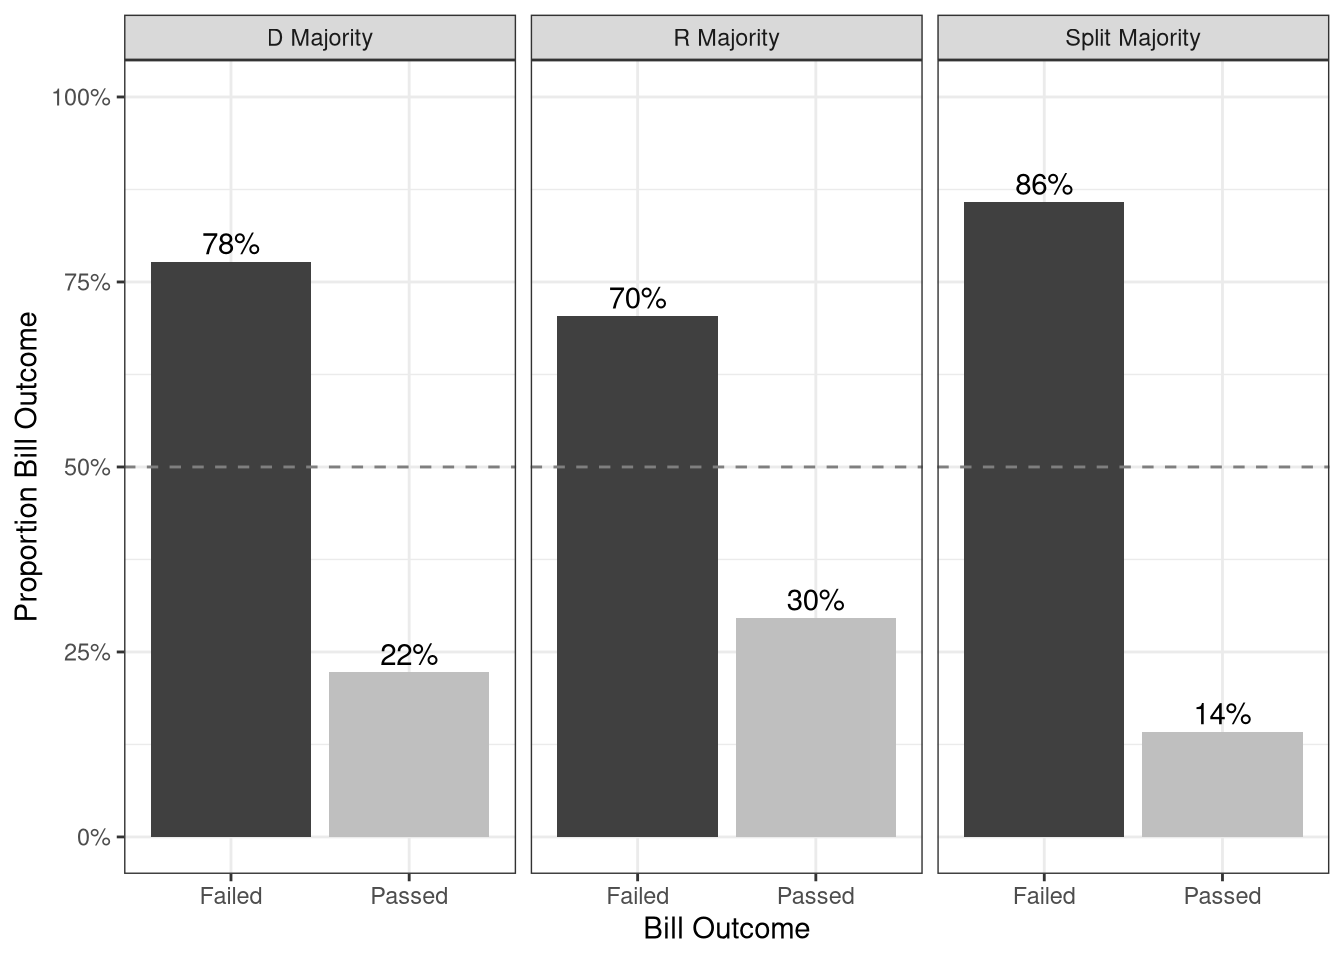
\includegraphics[width=0.95\linewidth]{Shor-Book_files/figure-latex/unnamed-chunk-4-1} \caption{Bill Outcomes}\label{fig:unnamed-chunk-4}
\end{figure}

\hypertarget{sponsorship}{%
\subsection{Sponsorship}\label{sponsorship}}

We won't get very far without understanding bill content. Different types of bills succeed and fail at different rates.

We begin our analysis by tracing bill histories as a function of bill content. But this is a big challenge with over 100,000 bills in the data. What we would like to know is what these bills are likely to do if translated into law. As a proxy measure for bill content, I use measures related to the bill sponsors. After all, writing and sponsoring bills is a purposive act (which has been used in the literature as a signal of legislator ideology). Legislators have a policy objective in addition to other reasons they might have for advancing legislation.

\hypertarget{sponsorship-by-party}{%
\subsection{Sponsorship by Party}\label{sponsorship-by-party}}

The first measure I propose is sponsor partisanship, which I divide into three categories: Democratic-only (D), Republican-only (R), and bipartisan (B). I expect that bills solely sponsored by partisans who match the partisanship of legislatures will be more likely to pass than those who don't match the partisanship. My expectation of bipartisan legislation is that it will do better than minority party-only sponsored bills, but not as well as the majority-party only bills. But this expectation changes for split legislatures, where bipartisanship will be a critical strength to manage the shoals of partisan conflict between the chambers.

Unified partisan legislatures show a native advantage for bill introductions to the majority party, though this advantage is most pronounced for Democratic legislatures. Perhaps unsurprisingly as well, split legislatures are more evenly split in bill sponsorship.

\begin{figure}
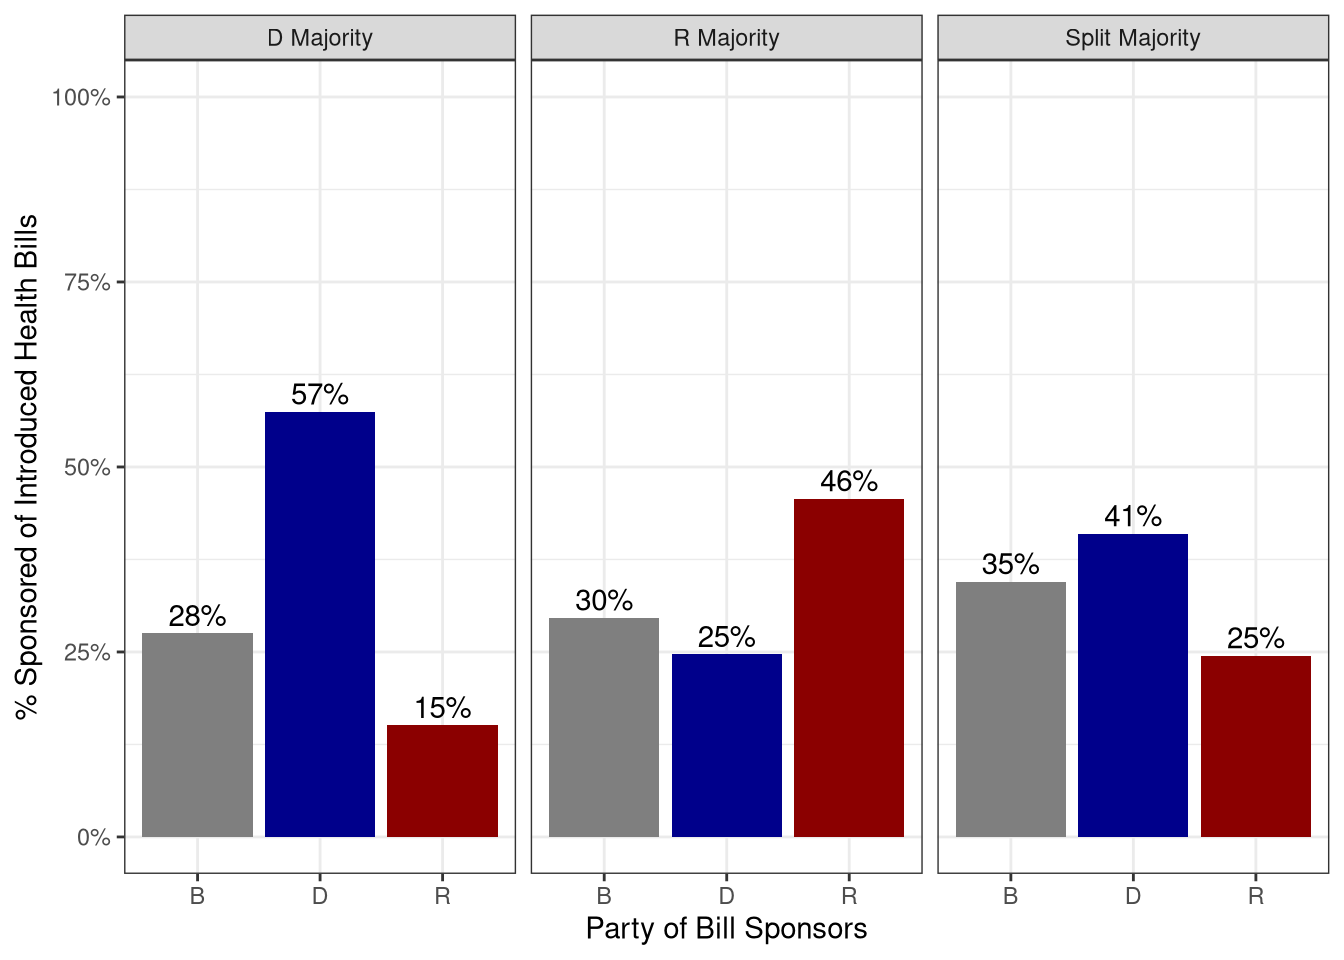
\includegraphics[width=0.95\linewidth]{Shor-Book_files/figure-latex/unnamed-chunk-5-1} \caption{Introduced Bills by Sponsor Partisanship}\label{fig:unnamed-chunk-5}
\end{figure}

What about bills that actually passed? Unsurprisingly again, the modal passed bill in unified legislatures is from the party in control. However, notice the relative success of Democratic bills in Republican legislatures compared with Republican bills in Democratic legislatures. Note, too, the large number of passed bipartisan bills in all types of legislatures.

\begin{figure}
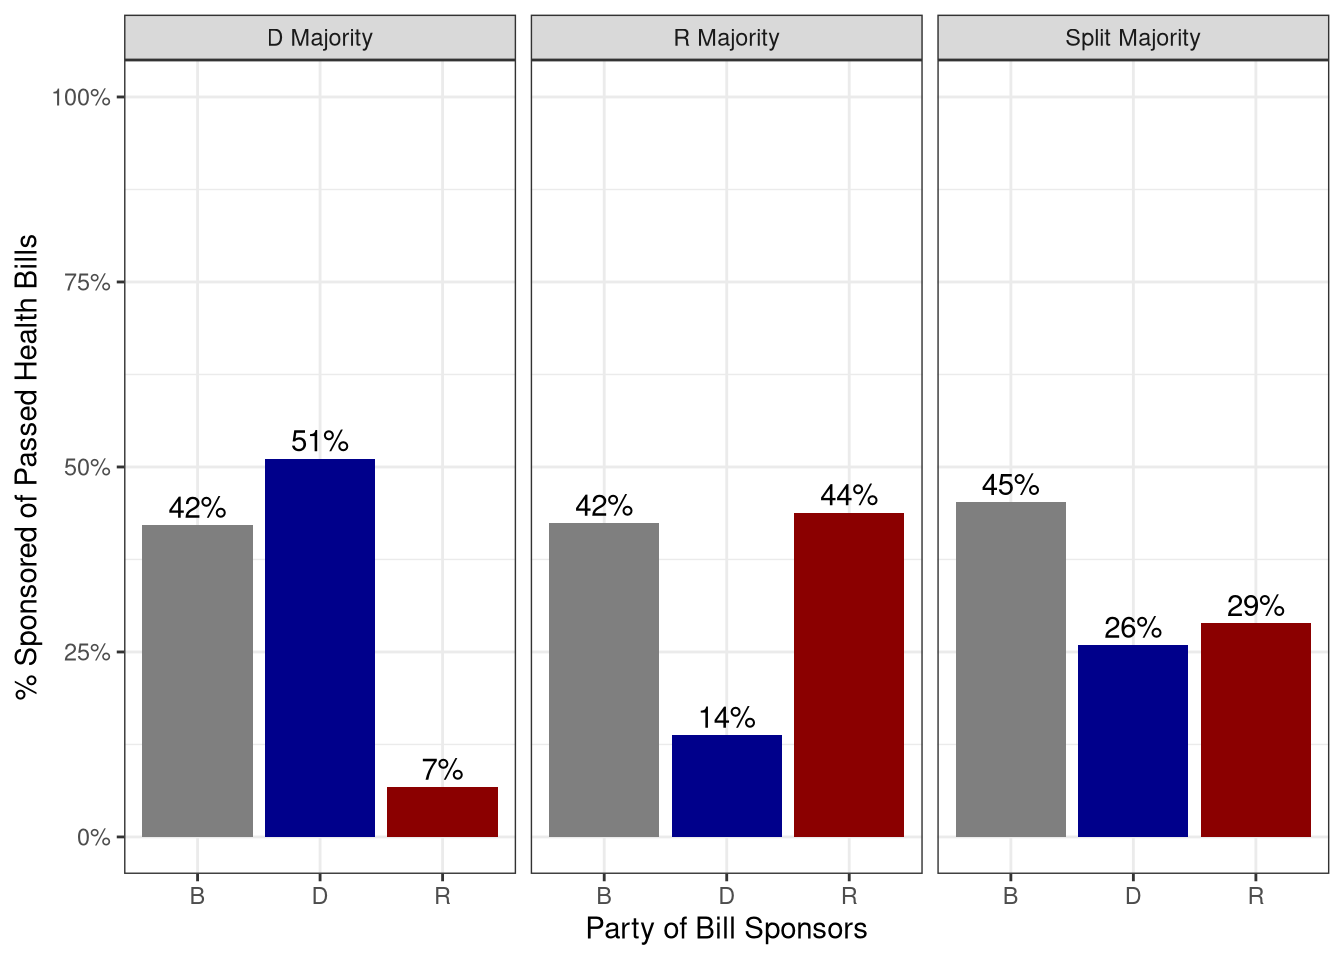
\includegraphics[width=0.95\linewidth]{Shor-Book_files/figure-latex/unnamed-chunk-6-1} \caption{Passed Bill Sponsorship Rates}\label{fig:unnamed-chunk-6}
\end{figure}

We can see how well bipartisan bills do when we look at hit rate of bills passed by partisanship. In fact, bipartisan bills pass at higher rates in unified majority legislatures than they do in split majority states.

\begin{figure}
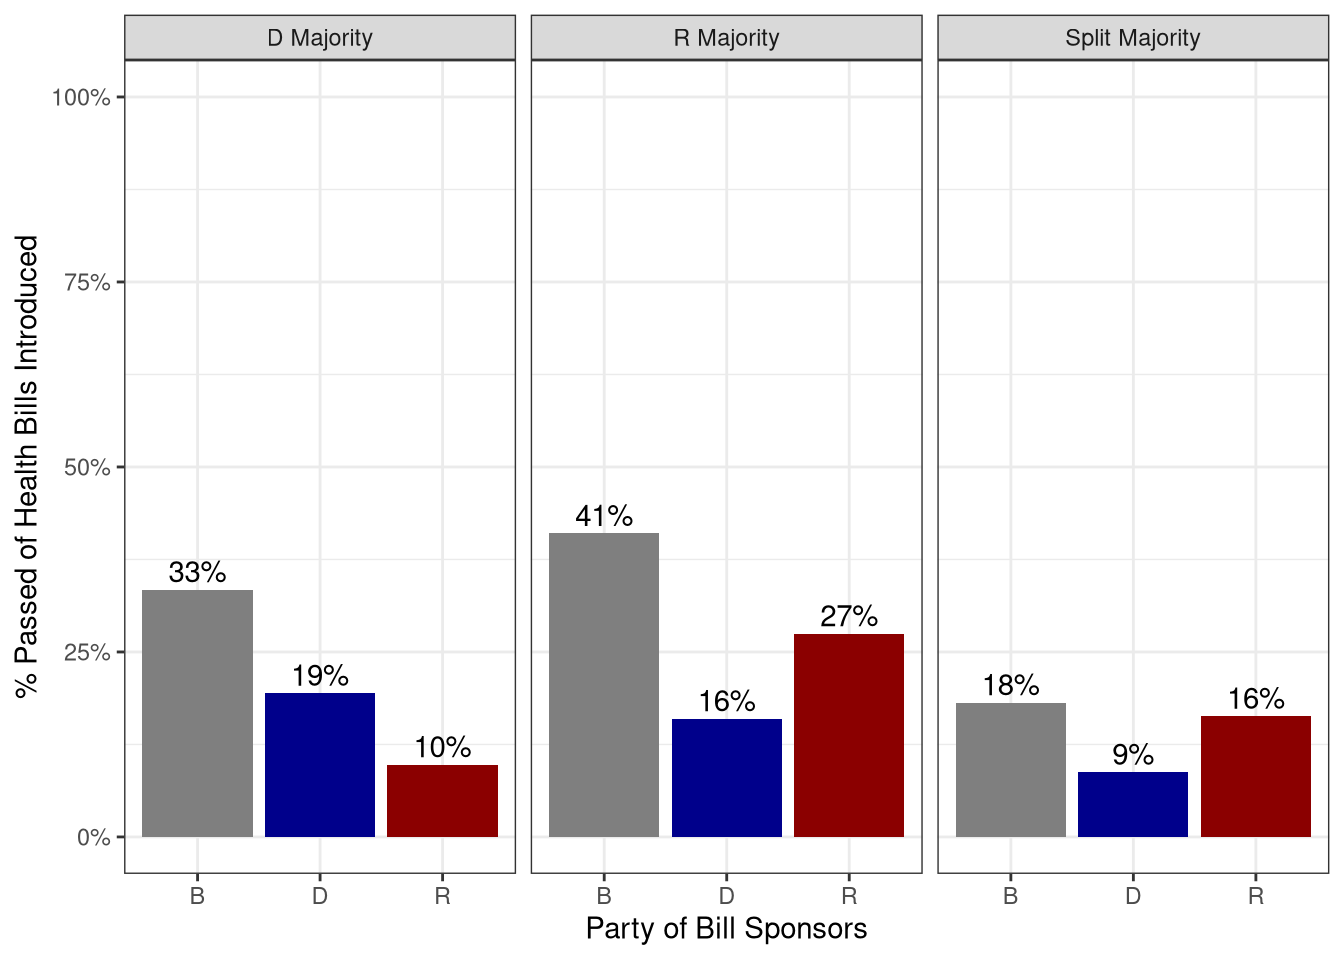
\includegraphics[width=0.95\linewidth]{Shor-Book_files/figure-latex/unnamed-chunk-7-1} \caption{Hit Rate of Sponsored Bills}\label{fig:unnamed-chunk-7}
\end{figure}

\begin{itemize}
\tightlist
\item
  Challenging when there are \textgreater{} 50,000 bills in the data
\item
  Proxy measure: Ideology of the median sponsor
\item
  Divided into terciles based on all unique legislators
\end{itemize}

\hypertarget{sponsor-ideology}{%
\subsection{Sponsor Ideology}\label{sponsor-ideology}}

Sponsor party, of course, is a crude measure of bill content. While still extremely useful as a typology, there is substantial internal ideological heterogeneity in modern American political parties (reference Shor and McCarty 2022, Shor and McCarty 2011). Modern ideal point estimation techniques (Shor and McCarty 2011, Clinton et al 2014) allow us to measure the latent concept of ideology using the observed roll call votes of legislators with an extremely finely-grained continuous measure.

Assuming that legislators have at least a major objective in moving policy in their preferred direction (``ideal point''), I use sponsor ideology as a second proxy measure of bill content.

Democratic chambers feature lots of liberal and moderate bill introductions, while Republican legislatures show no special place for conservative bills. In fact, there is not much difference between Republican and split majority legislatures.

\begin{figure}
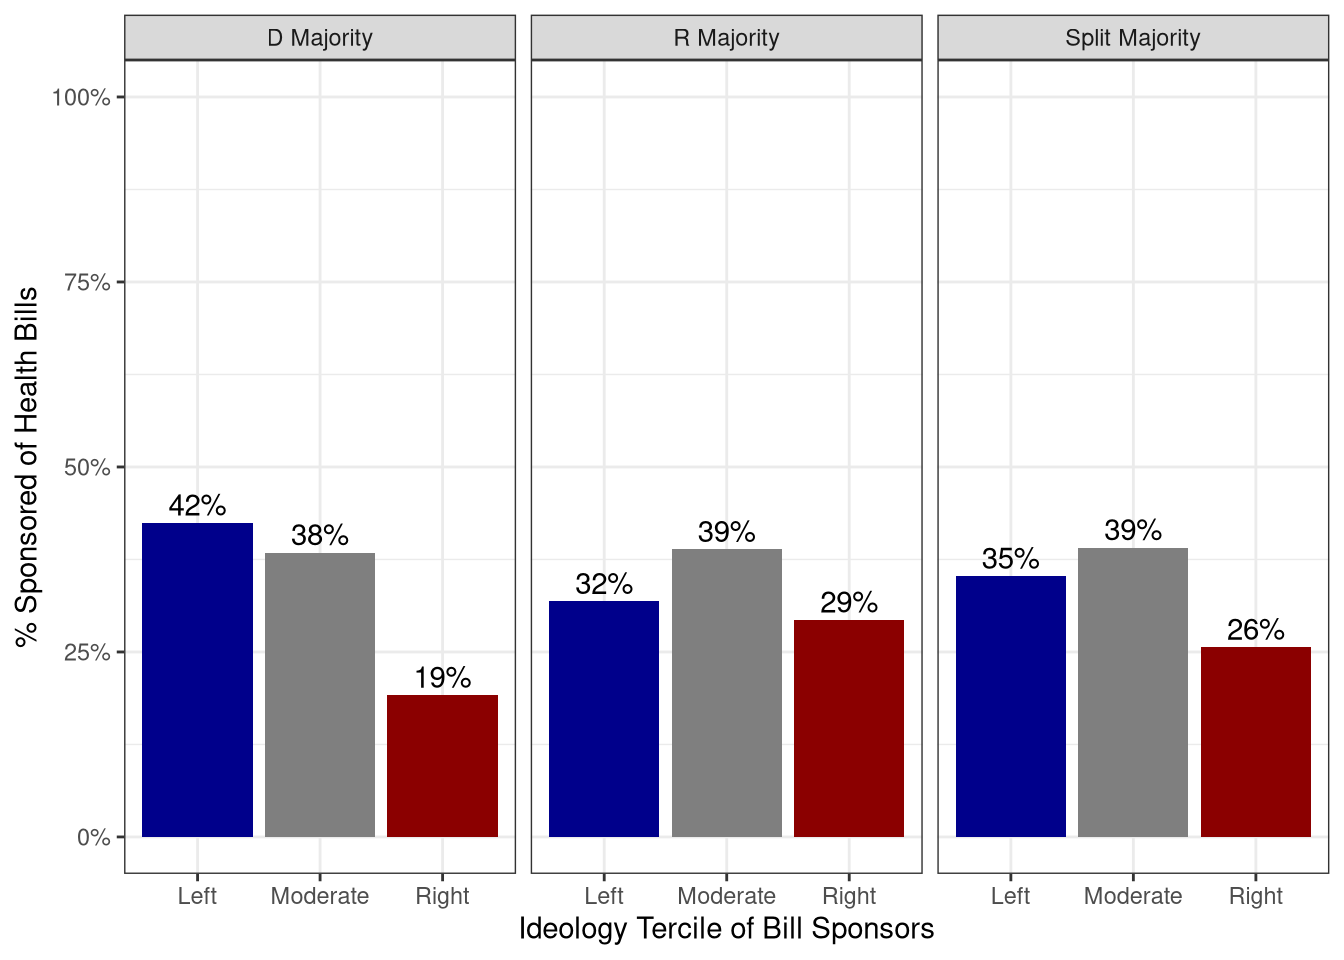
\includegraphics[width=0.95\linewidth]{Shor-Book_files/figure-latex/unnamed-chunk-8-1} \caption{Introduced Bills by Sponsor Ideology}\label{fig:unnamed-chunk-8}
\end{figure}

What about the minority of bills that actually passed? The disparity is even greater. Moderate bills tend to do very well in all types of legislative context. However, liberal bills do surprisingly well in Republican states, where they constitute only a few percentage points less than do conservative bills. In contrast, liberal bills in Democratic legislatures constitute nearly four times as many passed bills as conservative ones.

Republican majority chambers look no different than split majority chambers -- they both pass moderate bills, and a roughly even split of liberal and conservative bills. But Democratic states look very different.

\begin{figure}
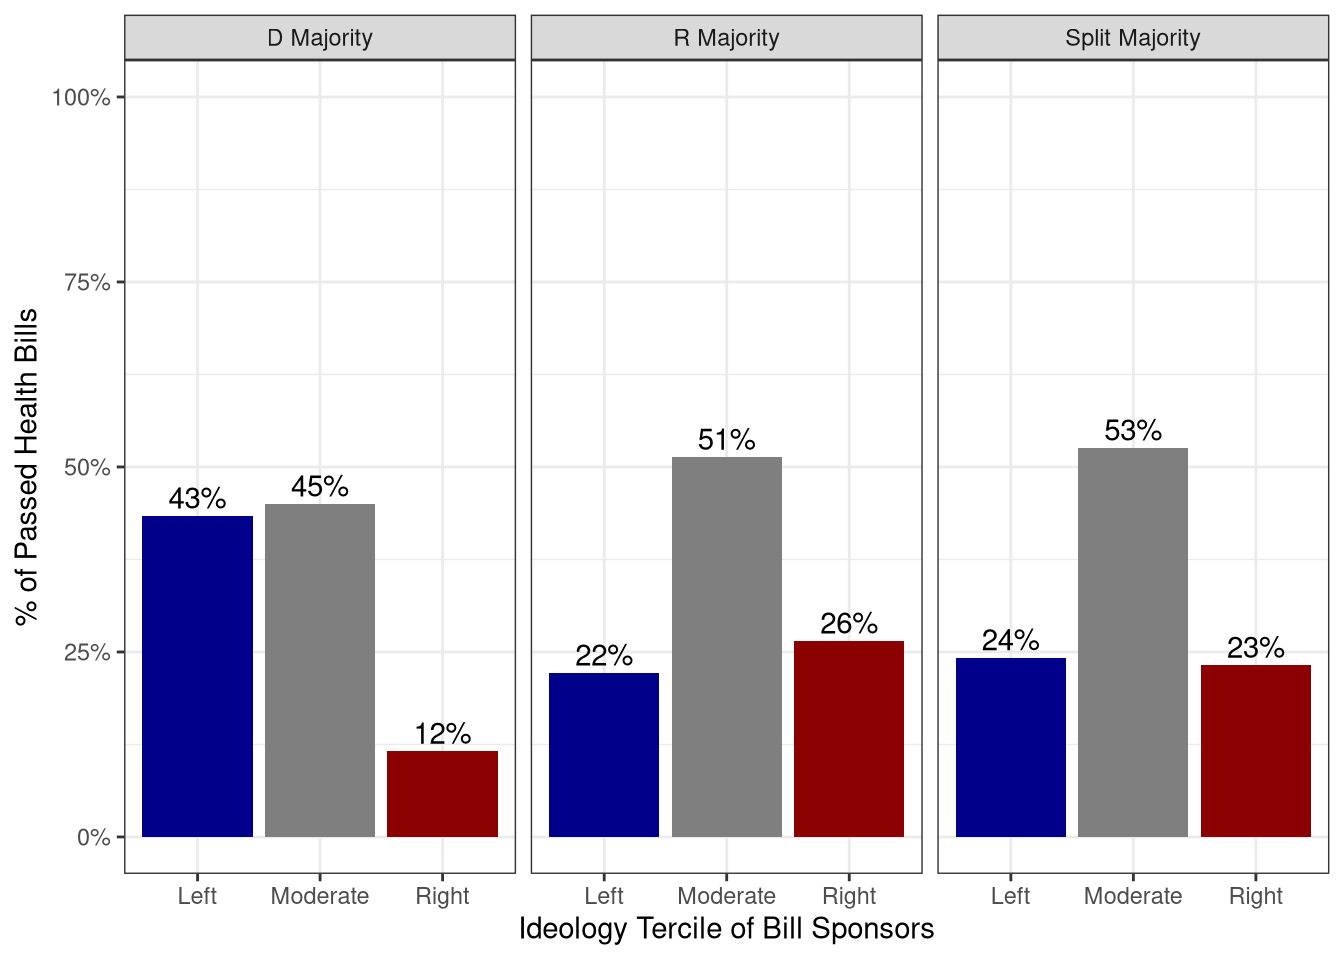
\includegraphics[width=0.95\linewidth]{Shor-Book_files/figure-latex/unnamed-chunk-9-1} \caption{Passed Bill Sponsorship Rates, By Ideology}\label{fig:unnamed-chunk-9}
\end{figure}

Next we look at hit rate of bills passed by ideology Moderate bills do very well, especially in Republican legislatures. And while liberal bills do almost as well in Republican legislatures as in Democratic ones, conservative bills do half as well in Democratic legislatures as compared with Republican ones.

\begin{figure}
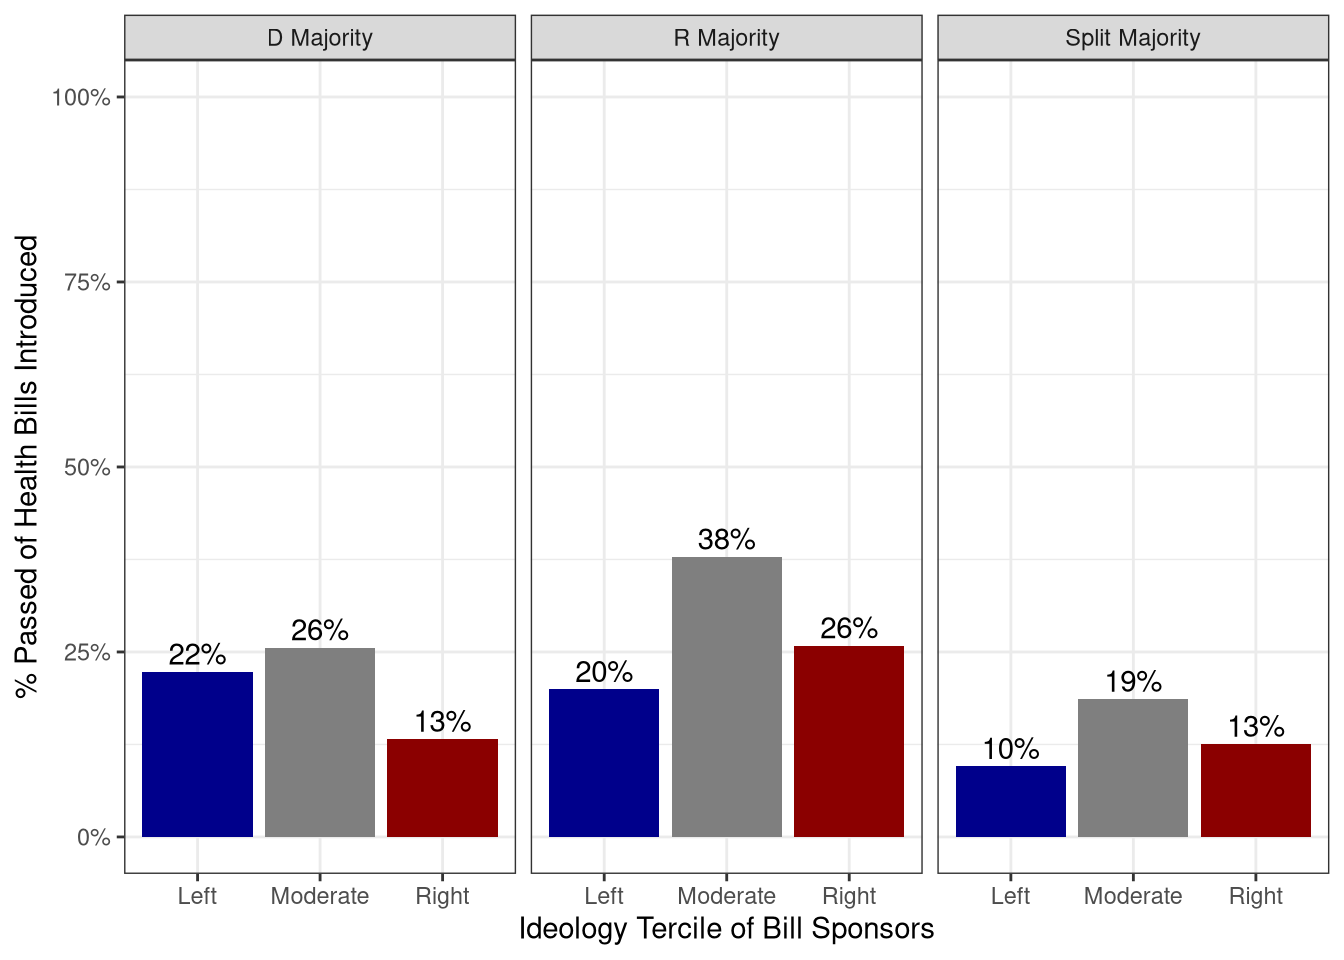
\includegraphics[width=0.95\linewidth]{Shor-Book_files/figure-latex/unnamed-chunk-10-1} \caption{Hit Rate of Sponsored Bills, by Sponsor Ideology}\label{fig:unnamed-chunk-10}
\end{figure}

\hypertarget{trends}{%
\section{Trends}\label{trends}}

The liberal advantage for health bills has existed for a decade and a half. The plot below shows the median sponsor ideology for passed bills in the entire United States. It has gone up and down a little over time, but has only ever been near zero once, in the wake of the 2016 elections. In other words, in every single year of the data, policy has been moving more leftward than rightward across the country as a whole.

\begin{figure}
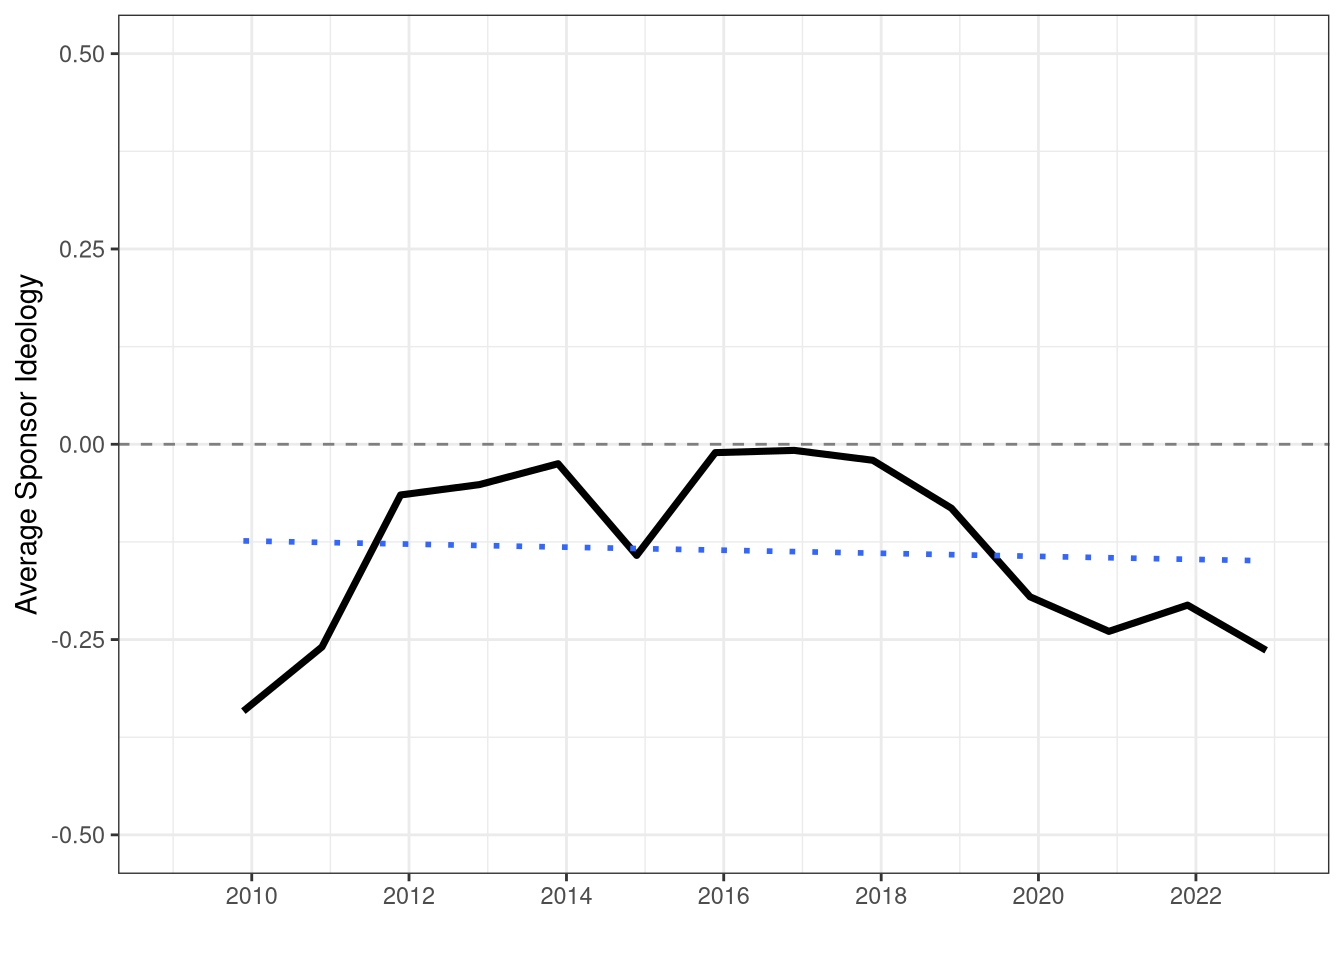
\includegraphics[width=0.95\linewidth]{Shor-Book_files/figure-latex/unnamed-chunk-12-1} \caption{Average Passed Bill Sponsor Ideology over Time}\label{fig:unnamed-chunk-12}
\end{figure}

Now we split the country into the familiar three categories. Examining the median sponsor ideology shows that bills sponsored in Democratic states are amongst the most liberal quarter in the state -- and have been getting more liberal over time.

Strikingly, the same is true for bills in Republican states. These are sponsored by the equivalent of the most liberal \textbf{quarter} of Republicans.

\begin{figure}
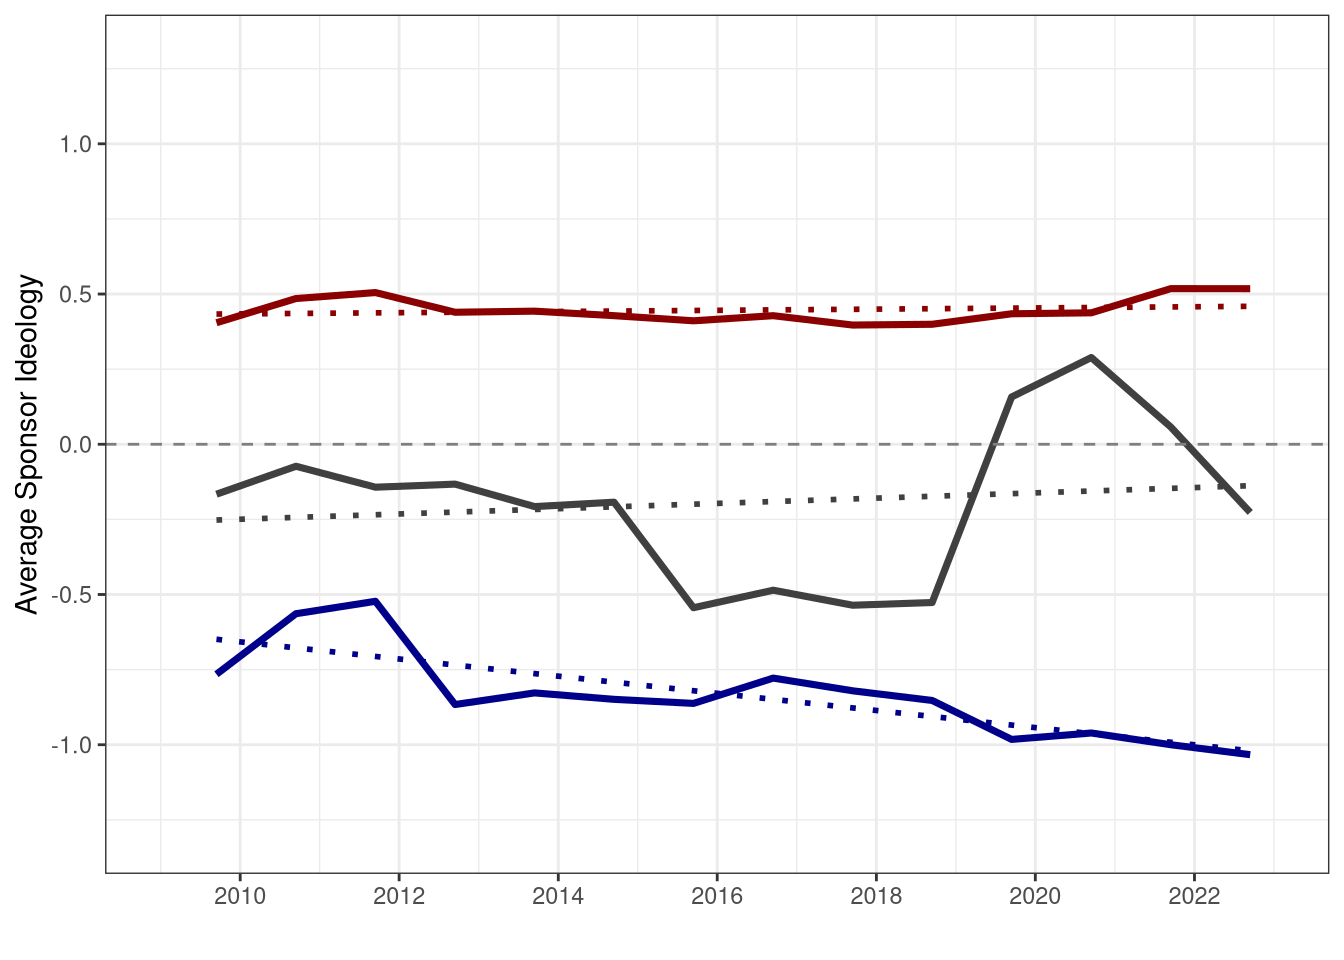
\includegraphics[width=0.95\linewidth]{Shor-Book_files/figure-latex/unnamed-chunk-13-1} \caption{Average Passed Bill Sponsor Ideology over Time by Majority Party}\label{fig:unnamed-chunk-13}
\end{figure}

\clearpage

\hypertarget{outcomes-by-state}{%
\section{Outcomes by State}\label{outcomes-by-state}}

Liberal bills do better in Democratic majority states than conservative bills in Republican majority chambers. In Republican majority chambers, moderate bills do almost as well as conservative ones; the same is not true in Democratic chambers.

We can see this by looking at the percentage of liberal bills passed in the states. Blue states are unsurprisingly the home of liberal bills.

\begin{figure}
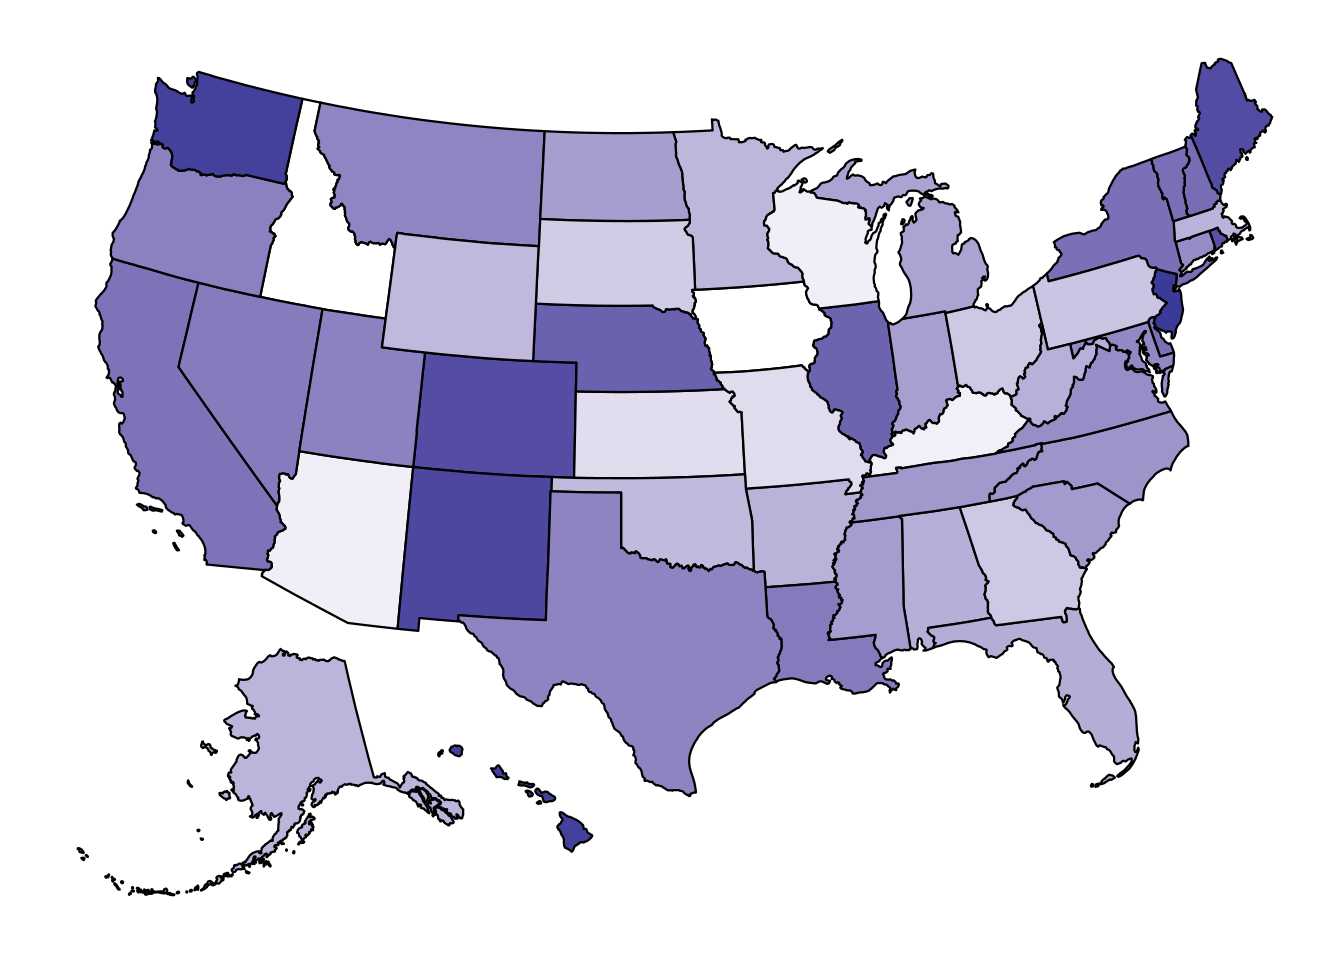
\includegraphics[width=0.95\linewidth]{Shor-Book_files/figure-latex/unnamed-chunk-15-1} \caption{Passed Liberal Bills by State}\label{fig:unnamed-chunk-15}
\end{figure}

While red states disproportionally feature the passage of conservative bills, it is not nearly to the commensurate degree.

\begin{figure}
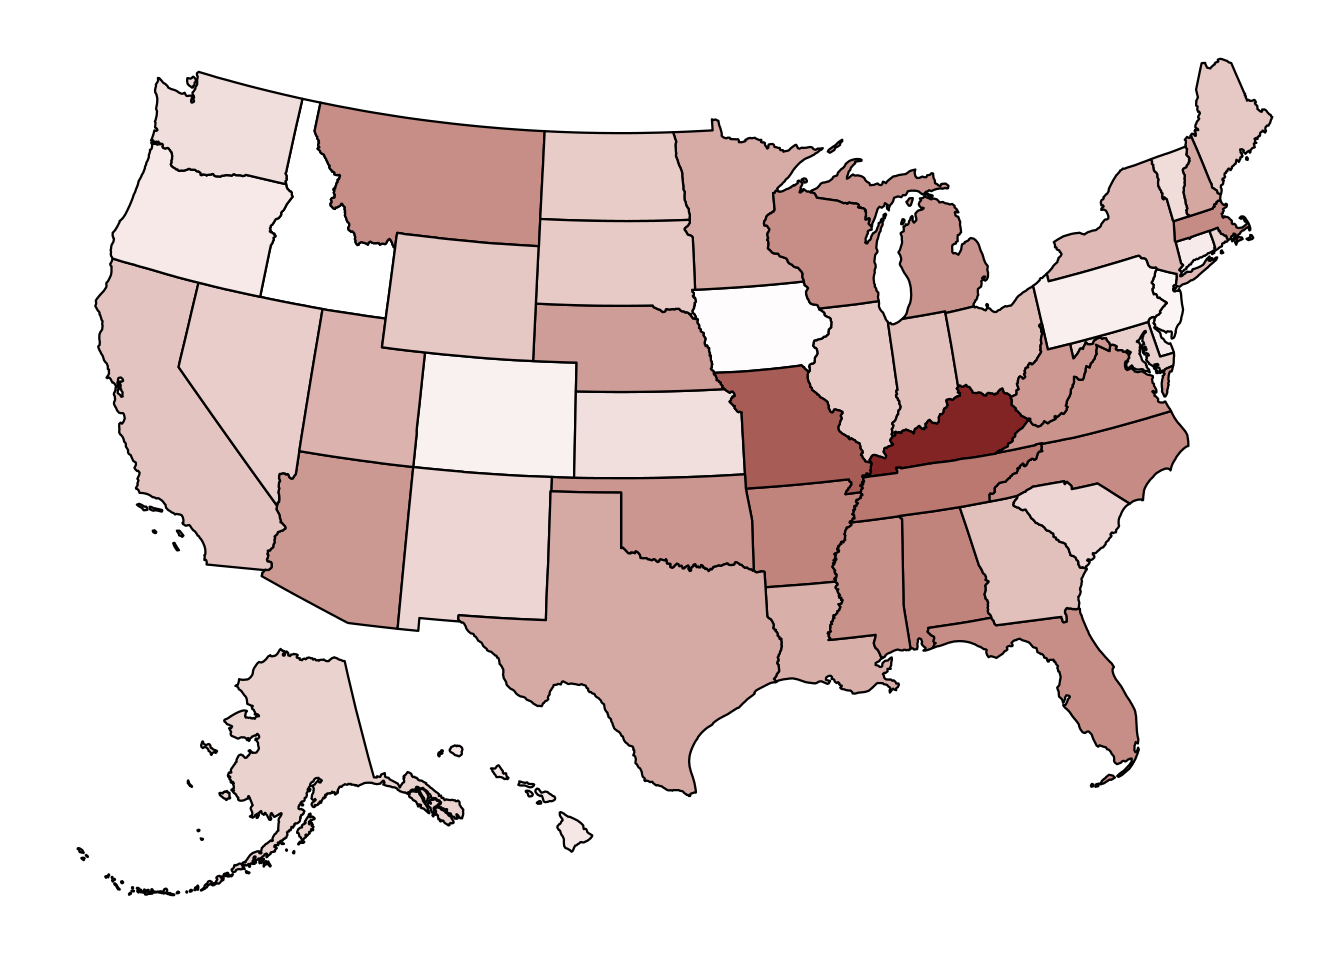
\includegraphics[width=0.95\linewidth]{Shor-Book_files/figure-latex/unnamed-chunk-16-1} \caption{Passed Conservative Bills by State}\label{fig:unnamed-chunk-16}
\end{figure}

Moving from a categorial to a continuous measure, we can see the median bill sponsor for passed bills across the country. Notice that, while the median passed bill in Texas and Florida is moderately conservative, the equivalent in California and New York is a strongly liberal bill.

\begin{figure}
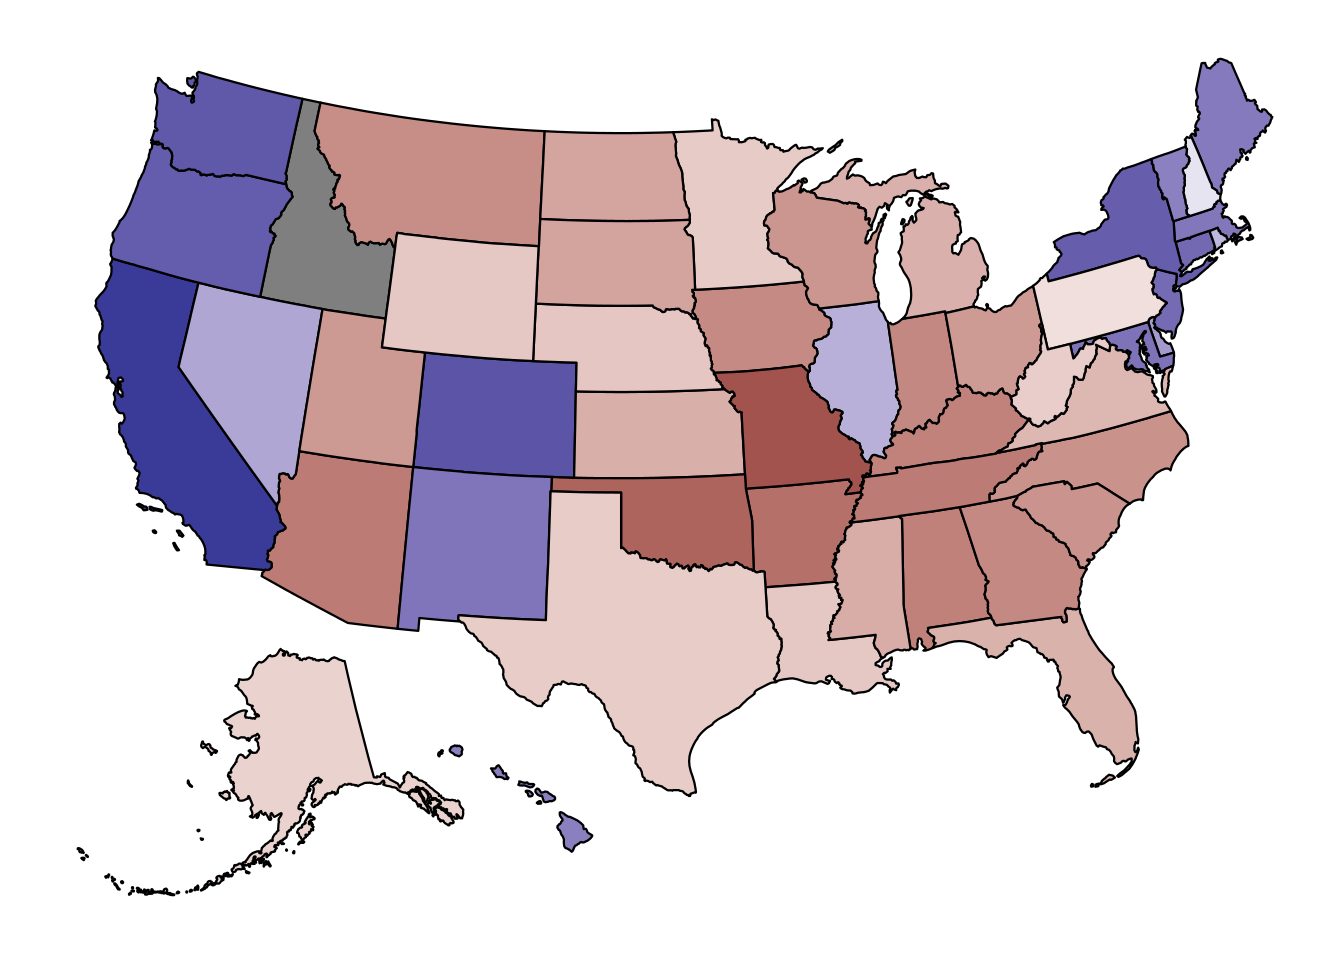
\includegraphics[width=0.95\linewidth]{Shor-Book_files/figure-latex/unnamed-chunk-17-1} \caption{Median Sponsor}\label{fig:unnamed-chunk-17}
\end{figure}

We combine the trend and state information in the following slopegraph. The figure in some respects is unsurprising. States like California and Washington State pass consistently liberal bills, while states like Arizona and Oklahoma pass consistently conservative bills. Other states exhibit understandable transitions, like Arkansas and West Virginia which have become much more conservative over time. What is surprising are large states like Florida and Texas passing health bills very often times authored by liberals.

\begin{figure}
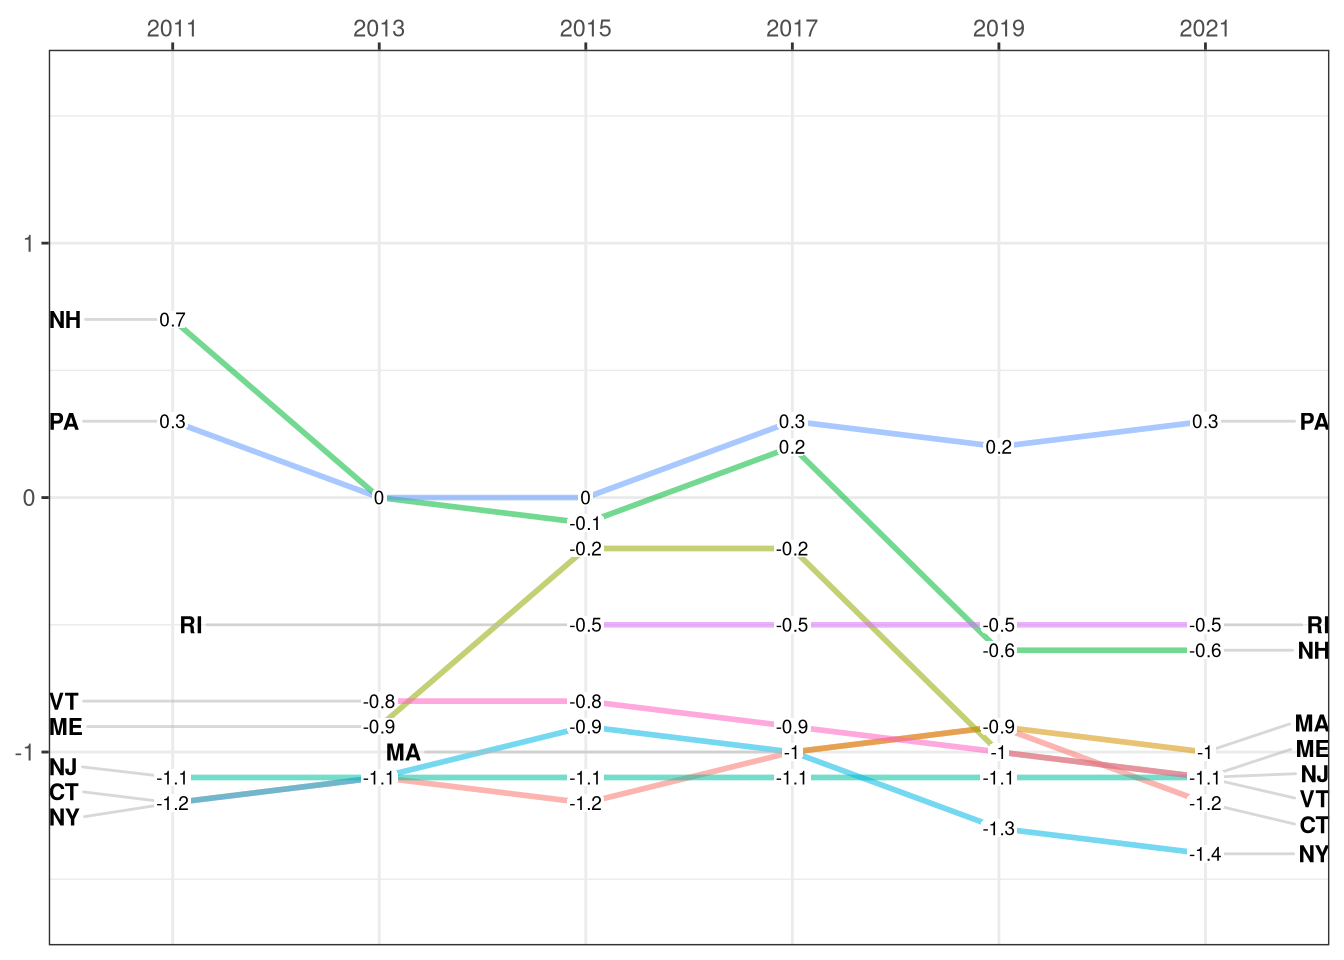
\includegraphics[width=0.95\linewidth]{Shor-Book_files/figure-latex/unnamed-chunk-19-1} \caption{State Bill Sponsorship Trends by State, Northeast}\label{fig:unnamed-chunk-19}
\end{figure}
\begin{figure}
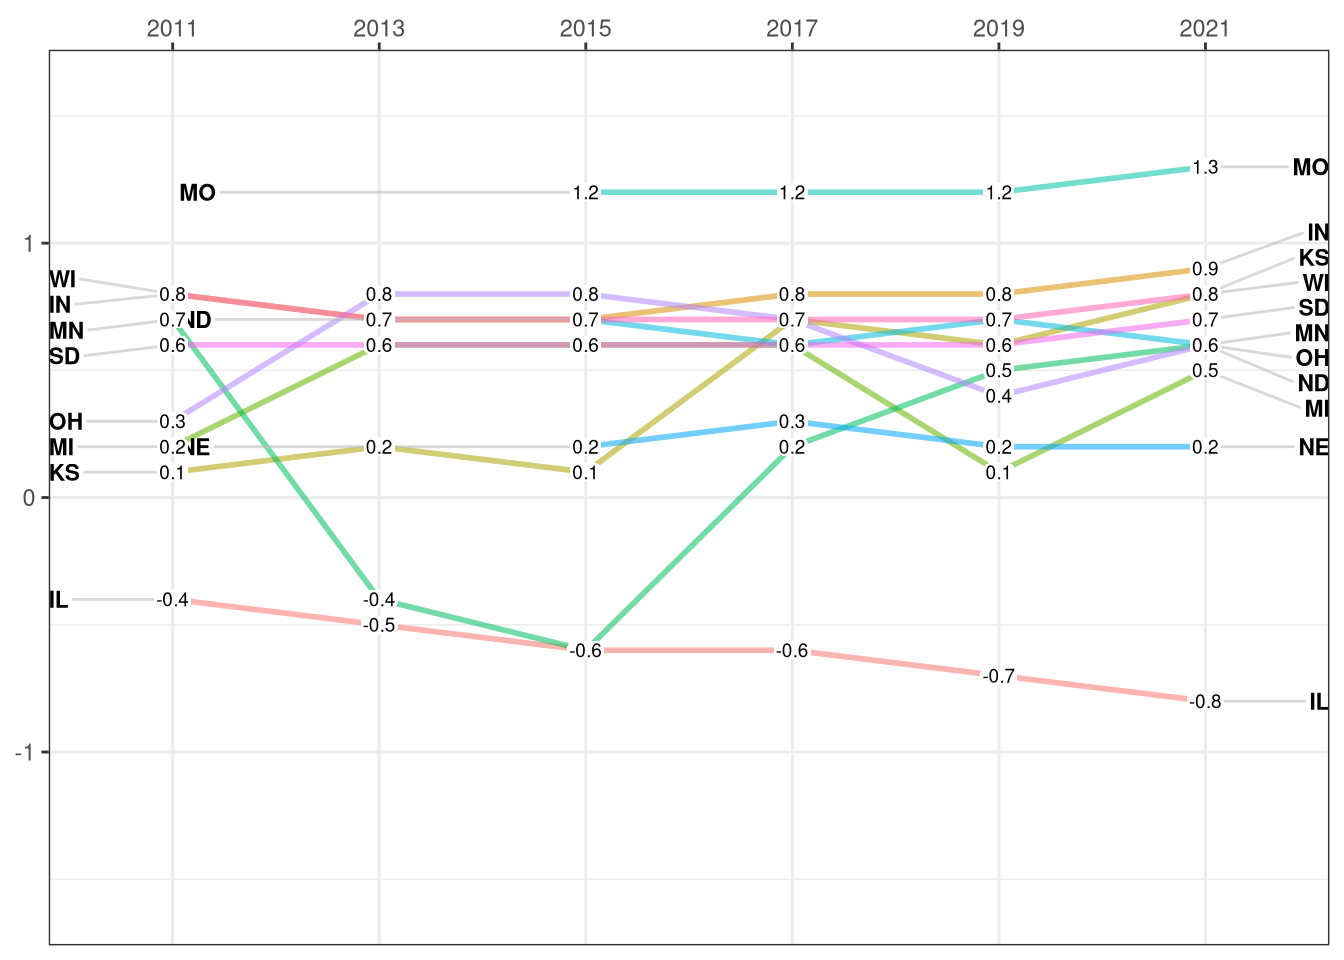
\includegraphics[width=0.95\linewidth]{Shor-Book_files/figure-latex/unnamed-chunk-20-1} \caption{State Bill Sponsorship Trends by State, Midwest}\label{fig:unnamed-chunk-20}
\end{figure}

\begin{figure}
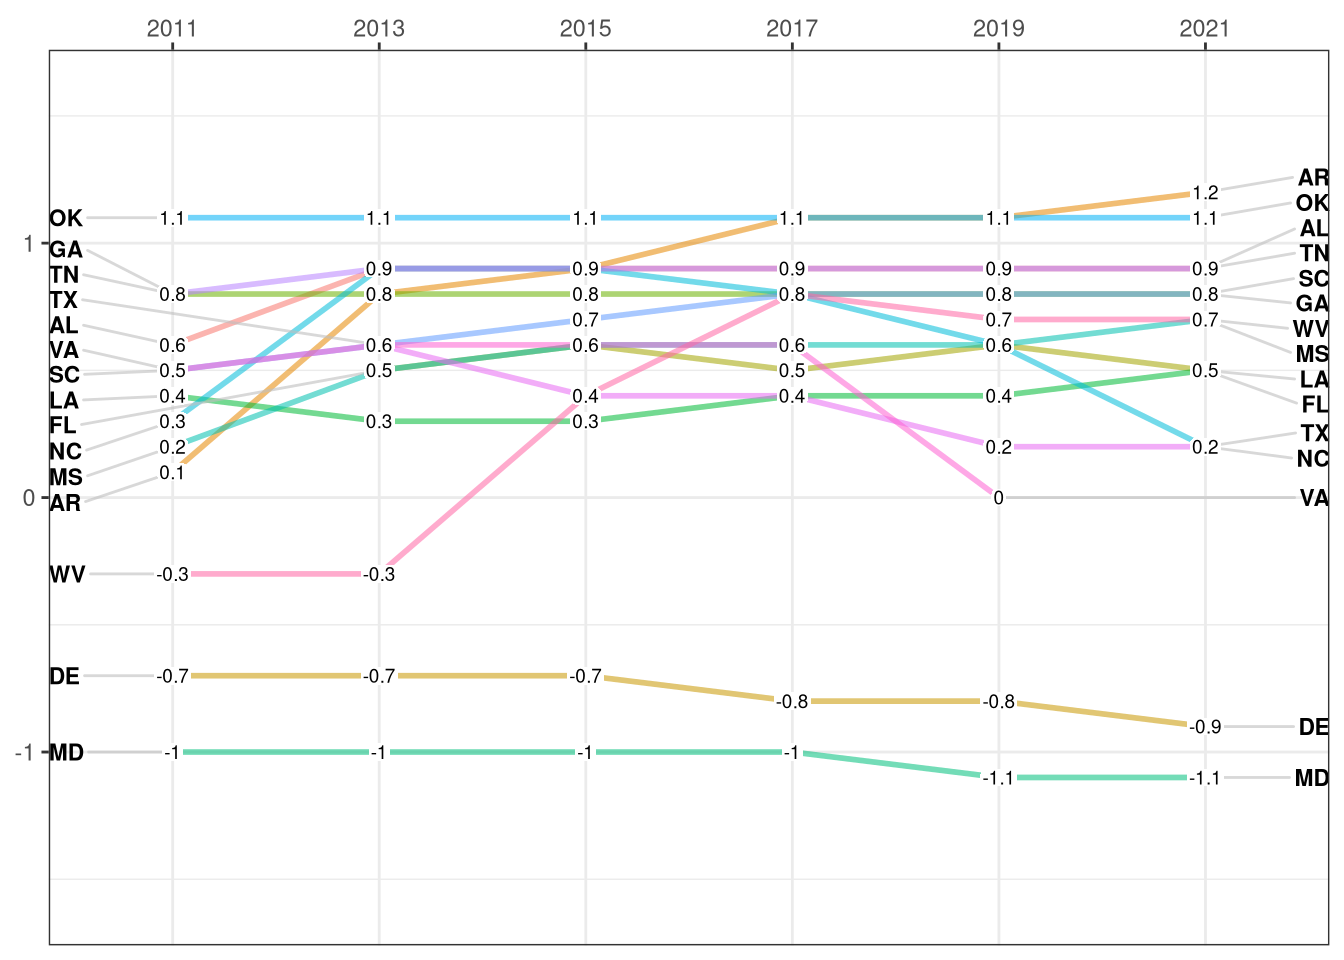
\includegraphics[width=0.95\linewidth]{Shor-Book_files/figure-latex/unnamed-chunk-21-1} \caption{State Bill Sponsorship Trends by State, South}\label{fig:unnamed-chunk-21}
\end{figure}

\begin{figure}
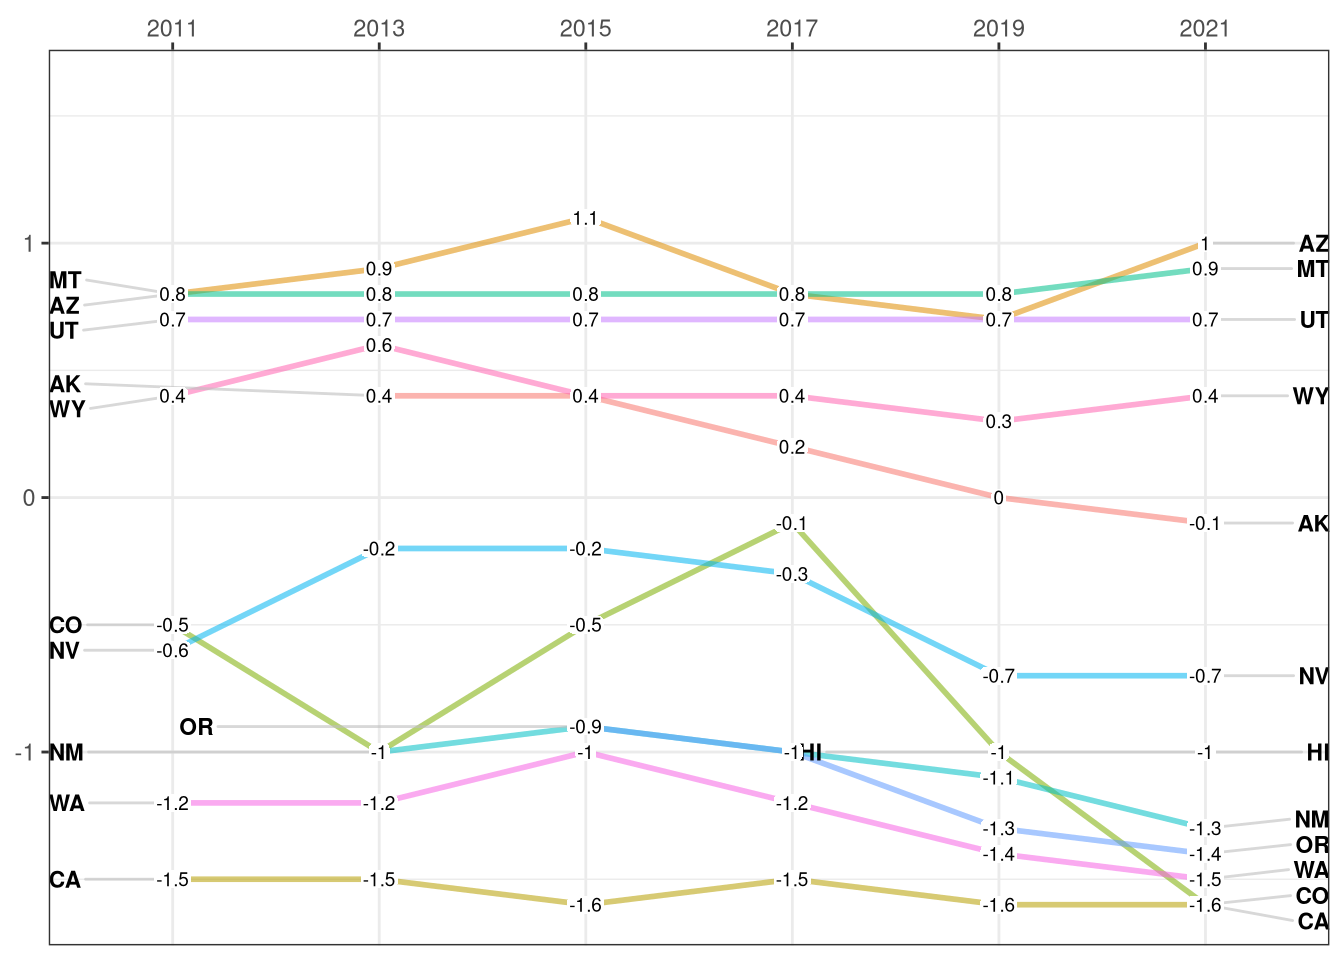
\includegraphics[width=0.95\linewidth]{Shor-Book_files/figure-latex/unnamed-chunk-22-1} \caption{State Bill Sponsorship Trends by State, West}\label{fig:unnamed-chunk-22}
\end{figure}

\hypertarget{partisan-asymmetry}{%
\section{Partisan Asymmetry}\label{partisan-asymmetry}}

\hypertarget{majority-rolls}{%
\subsection{Majority Rolls}\label{majority-rolls}}

Majority party rolls

\begin{itemize}
\tightlist
\item
  The norm for a majority party not to enable votes on bills that might pass without the support of the majority of the majority party
\item
  Sometimes called the ``Hastert rule''
\item
  Example of negative agenda control highlighted by cartel theory of Congressional organization
\item
  Only 41 violations between 1991 and 2018 in US House (0.6\% of all final passage roll calls)
\item
  What about the states? \citep{Anzia:2013}
\end{itemize}

The figure below shows the raw data. Of course, rolls happen in chamber votes. But in keeping with the focus on bills in this chapter, I aggregate to the bill level. Thus, the data shows the times rolls happen within any roll call on a given bill, as a percentage of all bills that ever had a floor vote.

\begin{figure}
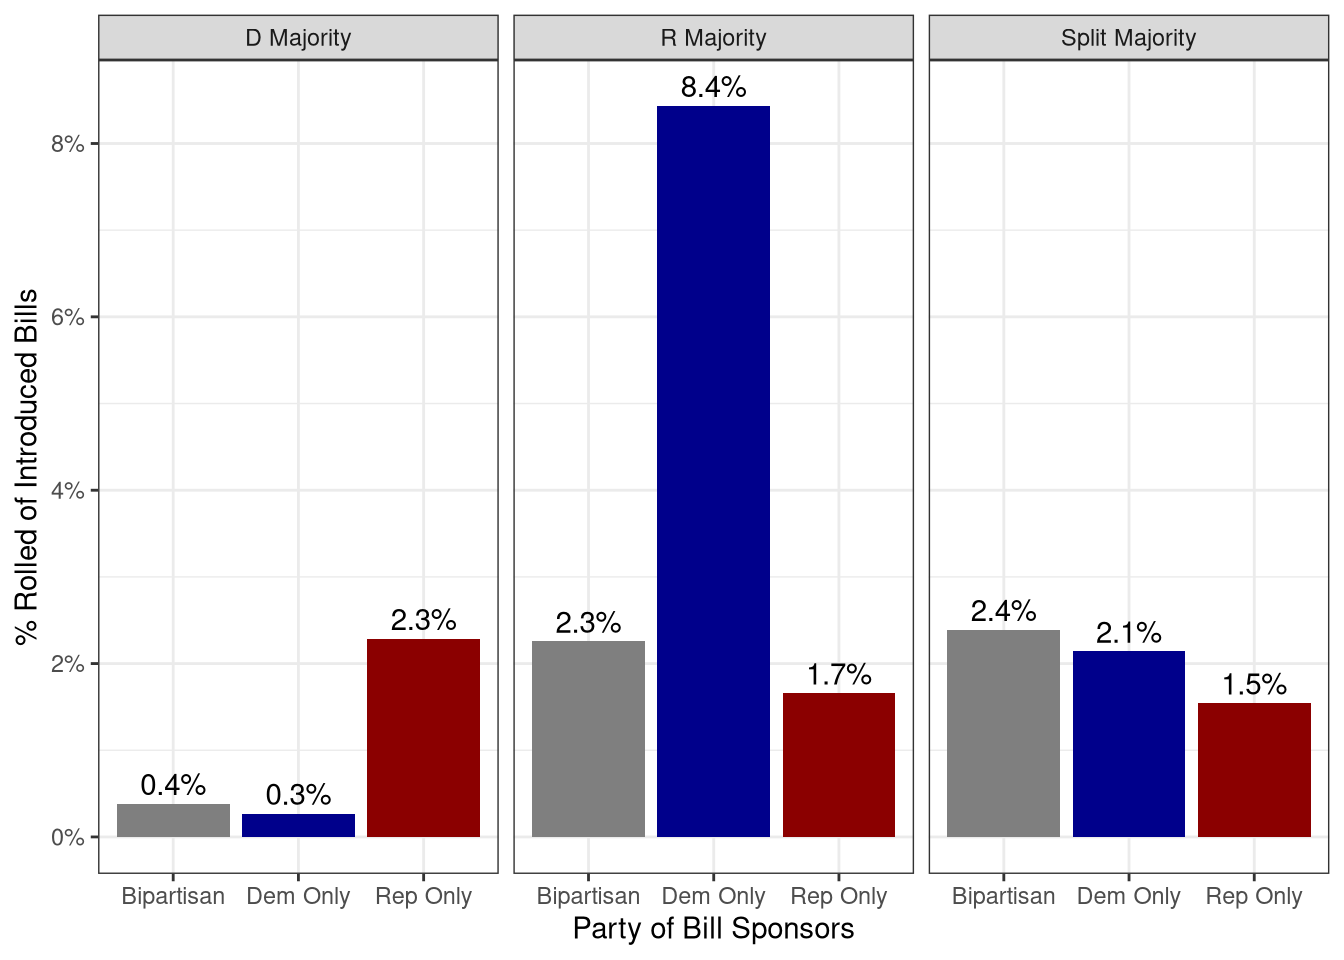
\includegraphics[width=0.95\linewidth]{Shor-Book_files/figure-latex/unnamed-chunk-23-1} \caption{Majority Party Rolls Vary by Party}\label{fig:unnamed-chunk-23}
\end{figure}

\hypertarget{describing-the-data---public-opinion}{%
\chapter{Describing the Data - Public Opinion}\label{describing-the-data---public-opinion}}

\hypertarget{data}{%
\section{Data}\label{data}}

Four waves of surveys have been conducted over the 2018-2022 time period, with a total of 39,098 respondents. Across all four waves, a total of 47 dichotomous survey responses about health-related policy issues, and 106 dichotomous survey responses about non-health related policy issues were asked. Of course, these questions were not all asked at the same time. The median number of health related questions that were answered was 16 (and 38 for non-health related questions).

\hypertarget{self-reported-vs-latent}{%
\section{Self-reported vs Latent}\label{self-reported-vs-latent}}

We estimate an ideal point based on two-item item-response model \citep{Clinton:2004} estimated in a single dimension. While typically ideal point models are estimated for politicians, they can be straightforwardly estimated for survey respondents \citep{Jessee:2012}. Recent research has shown that American public opinion is largely one-dimensional, like that of politicians \citep{Fowler:2022}.

\hypertarget{validating-the-measures}{%
\section{Validating the measures}\label{validating-the-measures}}

Table \ref{tab:ideol-corr} shows the correlations between the two self-reported measures of three-category party identification (Democrat, Republican, or true Independent\footnote{Leaners are included alongside partisans.}) and seven-category symbolic ideology (from strong liberal, or 1, to strong conservative, or 7), as well as the two latent measures of ideology.

The correlations are all in the expected range. Partisanship is strongly correlated with ideology, both symbolic and latent. Symbolic and latent ideology are also strongly correlated with each other.

\begin{table}

\caption{\label{tab:ideol-corr}Correlations between latent and self-reported measures of party and ideology}
\centering
\begin{tabular}[t]{>{\raggedright\arraybackslash}p{1.5in}>{\raggedleft\arraybackslash}p{0.75in}>{\raggedleft\arraybackslash}p{0.75in}>{\raggedleft\arraybackslash}p{0.75in}>{\raggedleft\arraybackslash}p{0.75in}}
\toprule
  & Party ID & Self-Reported Ideology & Latent Health Ideology & Latent Nonhealth Ideology\\
\midrule
Party ID & 1 & . & . & .\\
Self-Reported Ideology & \num{.59} & 1 & . & .\\
Latent Health Ideology & \num{.48} & \num{.44} & 1 & .\\
Latent Nonhealth Ideology & \num{.59} & \num{.60} & \num{.65} & 1\\
\bottomrule
\end{tabular}
\end{table}

Notice, however, that the correlations of \emph{health} ideology are substantially weaker with partisanship and symbolic ideology, as compared to \emph{non-health} ideology. We can see this graphically by plotting the density curves of both measures, broken out by partisanship (Figure \ref{fig:ideology-density-party}) and self-reported ideology (Figure \ref{fig:ideology-density-selfid}. Health ideology, then, is substantially \emph{less} polarized than ideology about non-health subjects.

More broadly, notice that ideology is substantially less polarized in general than the typical picture for politicians like state legislators and members of Congress, where there is either vanishingly little or even no overlap in the density curves for partisans. The public's ideology looks familiar, but it is in no way a mirror image of politicians' belief systems.

\begin{figure}
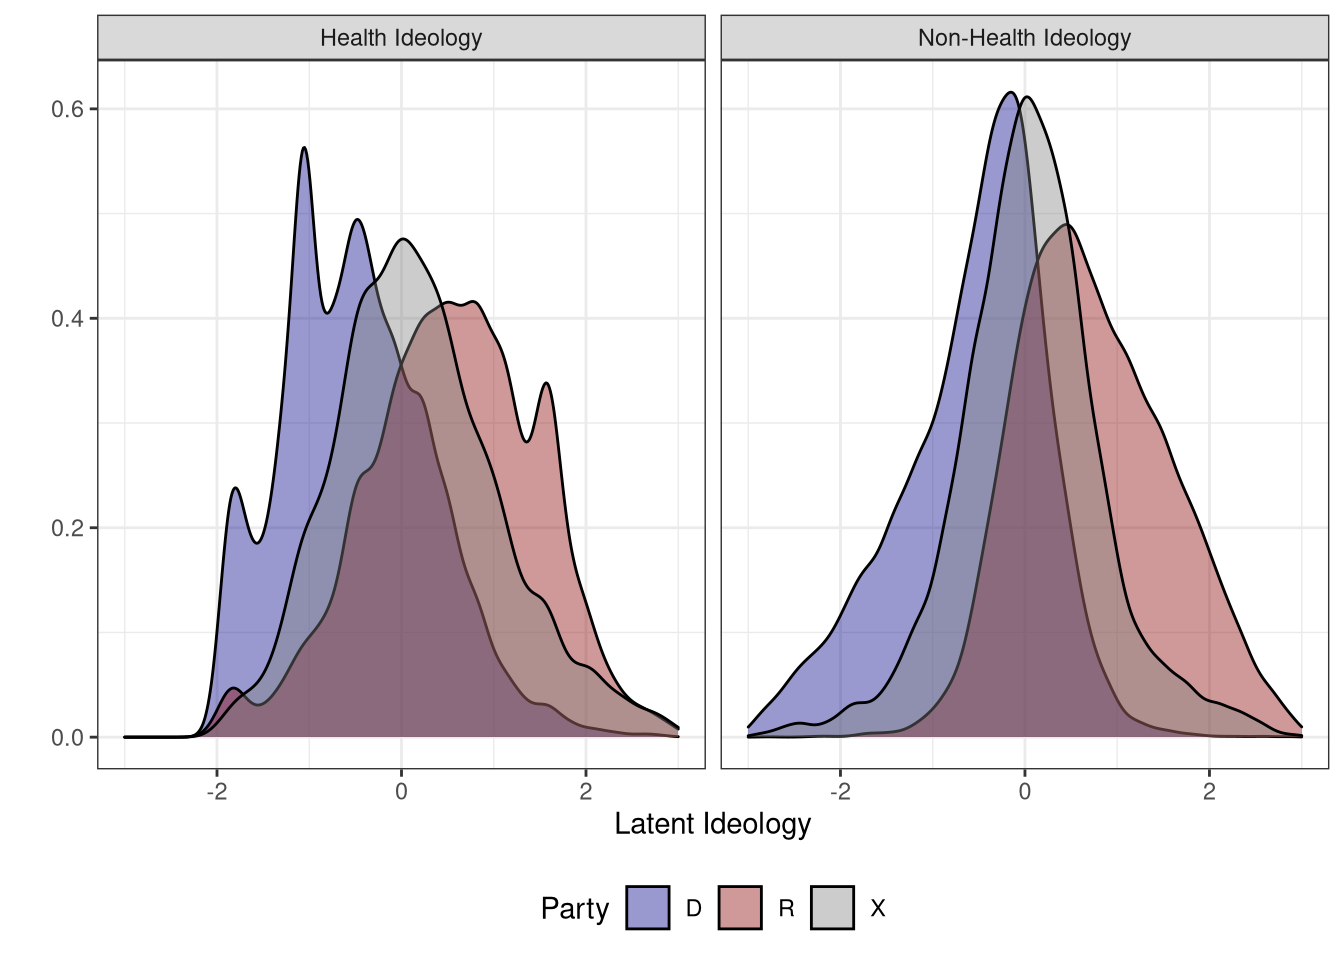
\includegraphics[width=0.95\linewidth]{Shor-Book_files/figure-latex/ideology-density-party-1} \caption{Health and Non-health latent ideology by 3-category party identification}\label{fig:ideology-density-party}
\end{figure}

\begin{figure}
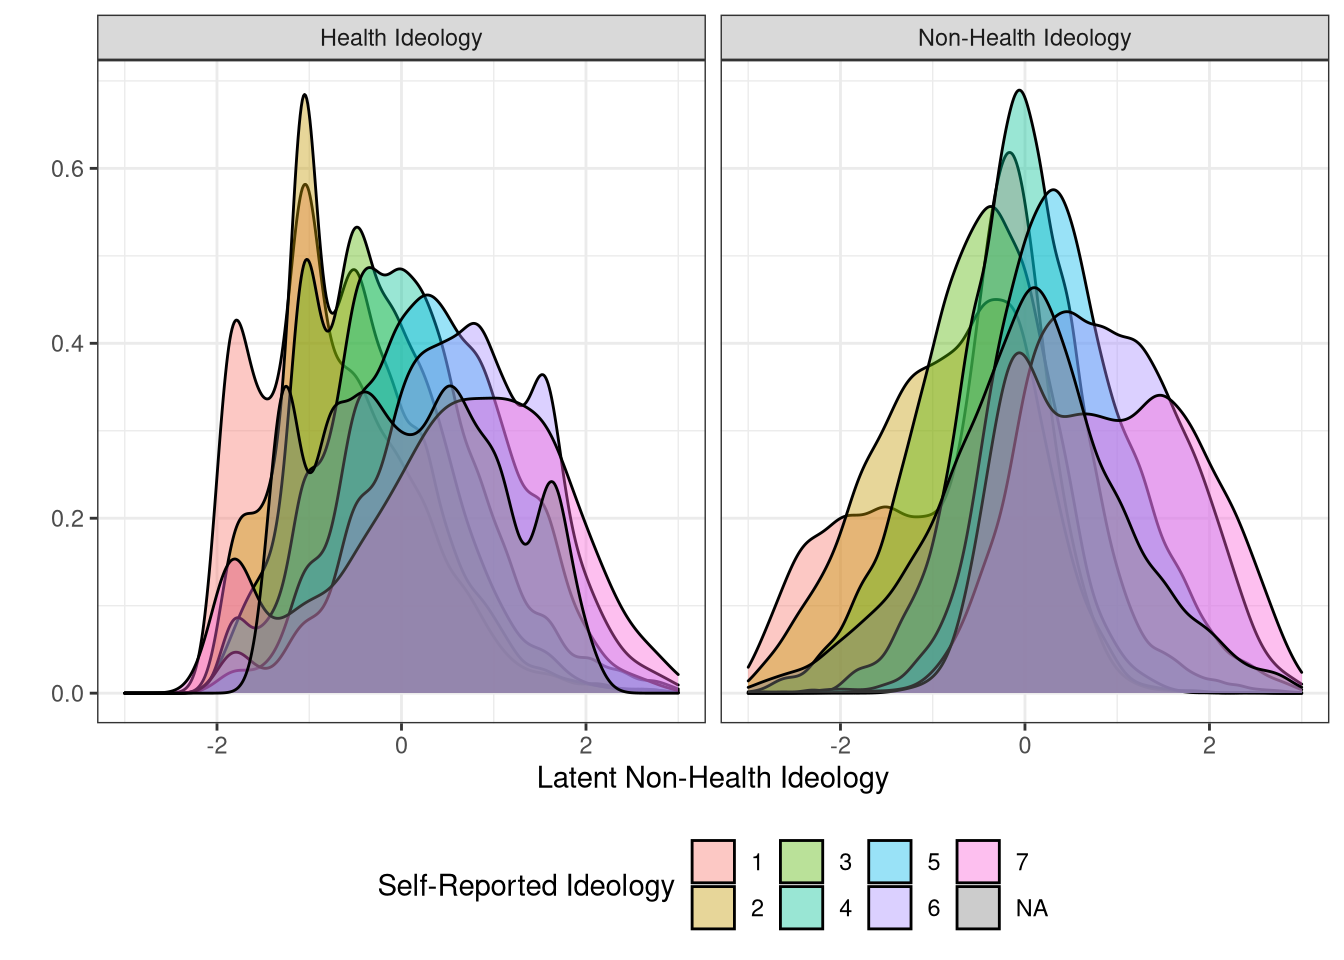
\includegraphics[width=0.95\linewidth]{Shor-Book_files/figure-latex/ideology-density-selfid-1} \caption{Health and Non-health latent ideology by 7-category self-reported ideology}\label{fig:ideology-density-selfid}
\end{figure}

\hypertarget{predicting-issue-opinion}{%
\subsection{Predicting issue opinion}\label{predicting-issue-opinion}}

I use the latent ideology measure as primary predictors in models of issue response. I regress them plus party and self-reported ideology on a variety of issue opinions. Table \ref{tab:acaopinion-model} shows several linear probability models. The first is generic Affordable Care Act approval. Next is opinion about expanding Medicaid within the respondent's state. Third is approval of Covid-19 vaccine mandates at schools. Finally, respondents are asked about the responsibility of states to cap the cost of insulin for diabetic patients. All in all, these various policy opinions tap a variety of issues, both those closely tied to partisanship and the first dimension of ideological conflict over the size and scope of the government (ACA Approval, Covid School Mandates) and those that are smaller in connection to partisanship or are less salient (Medicaid Expansion, Insulin Price Caps).

The coefficients are standardized in the \citet{Gelman:2008} fashion by dividing by two standard deviations to facilitate comparison of effect size within-model. As expected, the two more partisan issues show a greater effect of respondent partisan identification; in fact partisanship fades almost completely away for the latter two issues. For example, while Medicaid expansion or price caps on particular pharmaceutical products is often touted as a partisan issue, this simple model reveals that these issues are in fact much better described as ideological.

But what kind of ideology? Health-related latent ideology appears to be a much stronger predictor of policy opinions on important policy issues than does a more generalized latent ideology, or self-described ideological identification.

\begin{table}

\caption{\label{tab:acaopinion-model}ACA Issue Opinion Model}
\centering
\begin{tabular}[t]{lcccc}
\toprule
  & ACA Approval & COVID School Mandate & Medicaid Expansion & Insulin Price Cap\\
\midrule
Health Latent Ideology & \num{-0.340}*** & \num{-0.325}*** & \num{-0.541}*** & \num{-0.400}***\\
 & (\num{0.006}) & (\num{0.008}) & (\num{0.005}) & (\num{0.008})\\
Non-Health Latent Ideology & \num{-0.134}*** & \num{-0.058}*** & \num{-0.090}*** & \num{0.036}***\\
 & (\num{0.007}) & (\num{0.010}) & (\num{0.006}) & (\num{0.010})\\
Republican & \num{-0.253}*** & \num{-0.198}*** & \num{0.048}*** & \num{0.031}***\\
 & (\num{0.006}) & (\num{0.009}) & (\num{0.006}) & (\num{0.009})\\
Independent & \num{-0.091}*** & \num{-0.175}*** & \num{0.093}*** & \num{-0.043}***\\
 & (\num{0.006}) & (\num{0.009}) & (\num{0.005}) & (\num{0.009})\\
Self Reported Ideology & \num{-0.052}*** & \num{-0.070}*** & \num{0.034}*** & \num{-0.017}*\\
 & (\num{0.005}) & (\num{0.008}) & (\num{0.005}) & (\num{0.008})\\
\midrule
Num.Obs. & \num{29386} & \num{18358} & \num{30996} & \num{21211}\\
R2 & \num{0.431} & \num{0.290} & \num{0.428} & \num{0.152}\\
R2 Adj. & \num{0.431} & \num{0.290} & \num{0.428} & \num{0.152}\\
AIC & \num{23034.2} & \num{19966.1} & \num{18857.1} & \num{26621.6}\\
BIC & \num{23092.2} & \num{20020.8} & \num{18915.5} & \num{26677.3}\\
Log.Lik. & \num{-11510.100} & \num{-9976.061} & \num{-9421.551} & \num{-13303.804}\\
RMSE & \num{0.36} & \num{0.42} & \num{0.33} & \num{0.45}\\
\bottomrule
\multicolumn{5}{l}{\rule{0pt}{1em}+ p $<$ 0.1, * p $<$ 0.05, ** p $<$ 0.01, *** p $<$ 0.001}\\
\end{tabular}
\end{table}

\hypertarget{placebo-test}{%
\subsection{Placebo Test}\label{placebo-test}}

Is health-related ideology always and everywhere a better measure of policy attitudes? Certainly not. See the following set of placebo models as an example. This shows the exact same models as above, except with three non-health related policy measures as dependent variables. These including support for fracking, the death penalty, and concealled carry policy for guns. In all cases, non-health related ideology is strongly positively related with positions on these issues; that is, a respondent who is more conservative on this scale is more likely to take the conservative position on these three hot-button ideological issues. That's not a surprise. What is surprising is how the sign on health ideology flips in the opposite direction. Here, controlling for non-health ideology, health conservatism predicts a liberal position on these issues. Of course, this weird result is likely a statistical artifact of multicollinearity between the measures. Still, it shows that our health measure works appropriately in the correct context, and--just as important--works poorly in the incorrect context. It has passed the placebo test.

\begin{table}

\caption{\label{tab:unnamed-chunk-25}Placebo Issue Opinion Model}
\centering
\begin{tabular}[t]{lccc}
\toprule
  & Fracking & Death Penalty & Guns CC\\
\midrule
Health Latent Ideology & \num{-0.327}*** & \num{-0.245}*** & \num{-0.196}***\\
 & (\num{0.009}) & (\num{0.007}) & \vphantom{1} (\num{0.007})\\
Non-Health Latent Ideology & \num{0.642}*** & \num{0.421}*** & \num{0.376}***\\
 & (\num{0.011}) & (\num{0.008}) & \vphantom{1} (\num{0.008})\\
Republican & \num{-0.008} & \num{0.065}*** & \num{0.180}***\\
 & (\num{0.011}) & (\num{0.008}) & (\num{0.008})\\
Independent & \num{-0.097}*** & \num{0.010} & \num{0.096}***\\
 & (\num{0.010}) & (\num{0.008}) & (\num{0.008})\\
Self Reported Ideology & \num{0.030}*** & \num{0.023}** & \num{0.028}***\\
 & (\num{0.009}) & (\num{0.007}) & (\num{0.007})\\
\midrule
Num.Obs. & \num{15039} & \num{26654} & \num{26663}\\
R2 & \num{0.245} & \num{0.136} & \num{0.170}\\
R2 Adj. & \num{0.245} & \num{0.136} & \num{0.170}\\
AIC & \num{17514.0} & \num{33285.4} & \num{32518.0}\\
BIC & \num{17567.3} & \num{33342.7} & \num{32575.3}\\
Log.Lik. & \num{-8749.989} & \num{-16635.688} & \num{-16251.978}\\
RMSE & \num{0.43} & \num{0.45} & \num{0.45}\\
\bottomrule
\multicolumn{4}{l}{\rule{0pt}{1em}+ p $<$ 0.1, * p $<$ 0.05, ** p $<$ 0.01, *** p $<$ 0.001}\\
\end{tabular}
\end{table}

In sum, we will employ health related ideology as the best of related, but not identical, measures of health-related opinion by Americans.

\hypertarget{bill-models}{%
\chapter{Bill Models}\label{bill-models}}

\hypertarget{hypotheses}{%
\section{Hypotheses}\label{hypotheses}}

\begin{itemize}
\tightlist
\item
  Bill Content
  - More conservative bills will do better in R chambers, more liberal bills will do better in D chambers
\item
  Party

  \begin{itemize}
  \tightlist
  \item
    Given issue ownership, Dems want to pass health bills more than Reps
  \item
    Within-party, liberals should be more interested in passing health bills than conservatives
  \end{itemize}
\item
  Polarization

  \begin{itemize}
  \tightlist
  \item
    Polarization makes it more difficult to pass legislation
  \end{itemize}
\end{itemize}

\hypertarget{putting-it-all-together-bill-models}{%
\section{Putting it all together: Bill Models}\label{putting-it-all-together-bill-models}}

Table \ref{tab:billmodel} shows the results of our model for three configurations of legislatures: unified Republican, Unified Democratic, and split.

\hypertarget{modeling-choices}{%
\section{Modeling Choices}\label{modeling-choices}}

Because of the complexity in my data, my modeling strategy will to be to use a multilevel model, which can efficiently pool information at multiple levels of observation \citep{Raudenbush:2002, Gelman:2006}. They avoid a stark choice between complete pooling or ignoring contextual differences across units, or no pooling (often called fixed effects) which implies ignoring differences across units. The extent of the multilevel model's partial pooling is dictated by the data.

Varying intercepts for states and years account for unit- and time-specific heterogeneity in levels.

The specific model I use here is a simple linear probability model. While a generalized linear model like logit is typically used for a binary dependent variable like vote, the more modern approach is to use a simpler linear model as the gains in interpretability typically more than make up for the losses inherent in allowing the predicted values outside of the 0-1 range. I ran the generalized models as well, and include them in the appendix. These are qualitatively identical, and thus for simplicity I only show the former in the main results.

\hypertarget{bill-level-results}{%
\subsection{Bill level results}\label{bill-level-results}}

\begin{itemize}
\tightlist
\item
  Bill sponsored by conservatives suffer in Democratic states, and vice versa for Republican states; but the penalty is greater in the former for being ideologically out-of-step.
\end{itemize}

\begin{itemize}
\item
  Majority party conservatism is
\item
  Moderate Democratic are less likely to pass any bill than liberal Democratic legislatures
\item
  Conservative Republican legislatures are less likely to pass any bill than moderate Republican legislatures
\item
  Polarized legislatures are bad for the passage of any legislation, in either Republican or Democratic unified legislatures.
\end{itemize}

\begin{table}

\caption{\label{tab:billmodel}Bill Passage Models (All)}
\centering
\begin{tabular}[t]{lccc}
\toprule
  & Democratic Majority & Republican Majority & Split Majority\\
\midrule
Majority Party Conservatism & \num{-0.058}*** & \num{-0.080}*** & \num{0.006}*\\
 & (\num{<0.001}) & (\num{<0.001}) & (\num{0.020})\\
Sponsor Conservatism & \num{-0.053}*** & \num{0.041}*** & \num{0.009}*\\
 & (\num{<0.001}) & (\num{<0.001}) & (\num{0.021})\\
Democratic Only Sponsors & \num{-0.025}*** & \num{-0.138}*** & \num{-0.008}\\
 & (\num{<0.001}) & (\num{<0.001}) & (\num{0.367})\\
Republican Only Sponsors & \num{-0.037}*** & \num{-0.107}*** & \num{0.007}\\
 & (\num{<0.001}) & (\num{<0.001}) & (\num{0.491})\\
Polarization & \num{-0.064}*** & \num{-0.010} & \num{-0.007}\\
 & (\num{<0.001}) & (\num{0.353}) & (\num{0.702})\\
Sponsor Count & \num{0.003}*** & \num{0.004}*** & \num{0.002}***\\
 & (\num{<0.001}) & (\num{<0.001}) & \vphantom{1} (\num{<0.001})\\
Sponsor Ideological Range & \num{0.080}*** & \num{0.036}*** & \num{0.025}***\\
 & (\num{<0.001}) & (\num{<0.001}) & (\num{<0.001})\\
\midrule
Num.Obs. & \num{76642} & \num{76967} & \num{24203}\\
R2 Marg. & \num{0.063} & \num{0.084} & \num{0.019}\\
R2 Cond. & \num{0.277} & \num{0.199} & \num{0.375}\\
AIC & \num{65253.4} & \num{82975.1} & \num{11425.8}\\
BIC & \num{65364.3} & \num{83095.4} & \num{11531.1}\\
RMSE & \num{0.37} & \num{0.41} & \num{0.30}\\
\bottomrule
\multicolumn{4}{l}{\rule{0pt}{1em}+ p $<$ 0.1, * p $<$ 0.05, ** p $<$ 0.01, *** p $<$ 0.001}\\
\end{tabular}
\end{table}

We can plot the marginal effect of our key variables. Figure \ref{fig:sponsor-effect} shows the effect of bill (sponsor) conservatism and bill (sponsor) partisanship, separated by Democratic and Republican majorities. I drop showing split majorities, for which I do not have predictions for the key predictors (and which show mostly insignificant results for them).

Bill sponsored by conservatives suffer in Democratic states, and vice versa for Republican states; but the penalty is greater in the former for being ideologically out-of-step. Bipartisan bills do really well, and most especially in Republican legislatures.

\begin{figure}
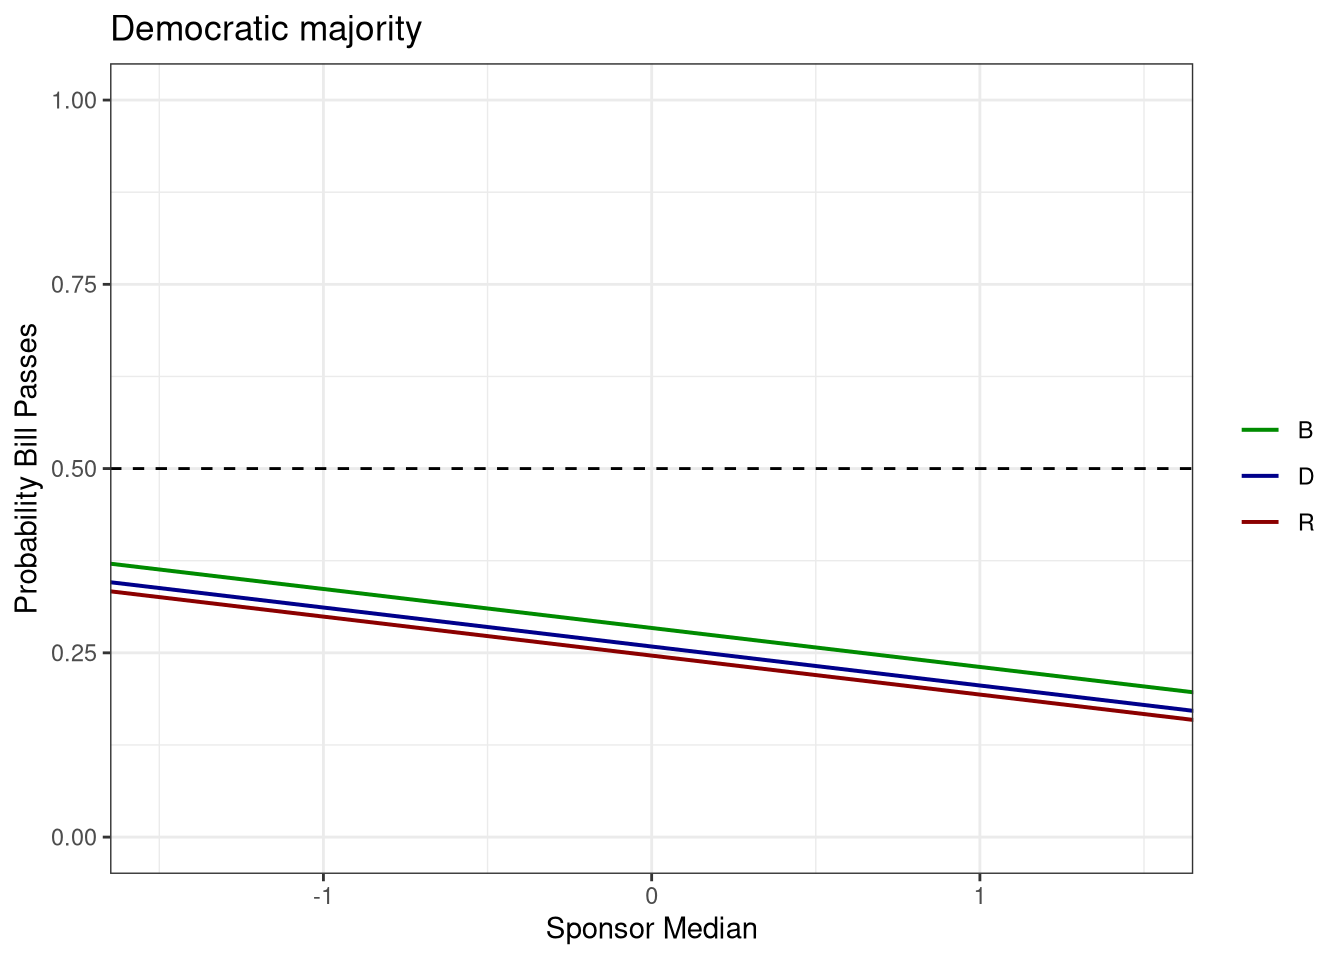
\includegraphics[width=0.5\linewidth]{Shor-Book_files/figure-latex/sponsor-effect-1} 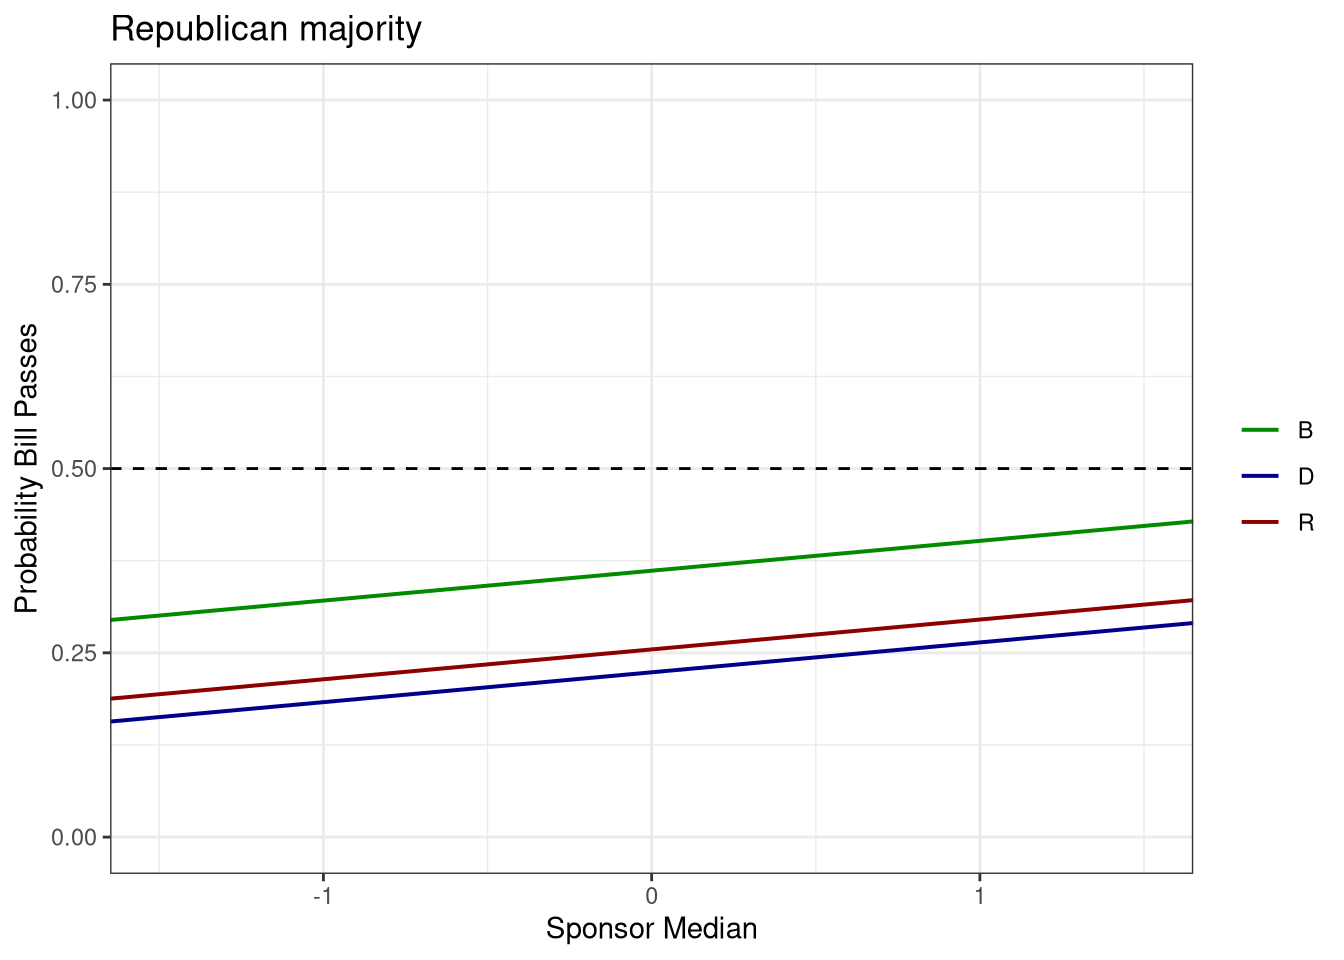
\includegraphics[width=0.5\linewidth]{Shor-Book_files/figure-latex/sponsor-effect-2} \caption{Passage probability as a function of sponsor ideology}\label{fig:sponsor-effect}
\end{figure}

\hypertarget{vote-models}{%
\chapter{Vote Models}\label{vote-models}}

\hypertarget{hypotheses-1}{%
\section{Hypotheses}\label{hypotheses-1}}

\begin{itemize}
\tightlist
\item
  Party

  \begin{itemize}
  \tightlist
  \item
    McConnell: top priority is making Obama a one-term president. Partisanship above all else.
  \item
    Teamsmanship is paramount; party pressure overrules individual preferences (Lee)
  \end{itemize}
\item
  Ideology

  \begin{itemize}
  \tightlist
  \item
    Individual policy preferences are paramount and almost always 1D (Poole and Rosenthal)
  \item
    Single spatial dimension accounts for nearly all votes in polarized times
  \item
    Ideological heterogeneity within parties is large (Shor and McCarty)
  \end{itemize}
\item
  Opinion

  \begin{itemize}
  \tightlist
  \item
    Election motive might pressure legislators
  \item
    But information about statehouse votes is very weak
  \end{itemize}
\end{itemize}

\hypertarget{putting-it-all-together-vote-models}{%
\section{Putting it all together: Vote Models}\label{putting-it-all-together-vote-models}}

\hypertarget{outcome-variable}{%
\subsection{Outcome Variable}\label{outcome-variable}}

The outcome variable is a yea or nay vote in a roll call on a bill sponsored by a liberal (NPAT common space ideal point \textless{} 0). This was done to flip the votes in a common direction.

\hypertarget{key-predictors}{%
\subsection{Key Predictors}\label{key-predictors}}

The key predictors are legislator ideology \citep{Shor:2011} and district ideology \citep{Tausanovitch:2013}.\footnote{These are described as ``conservatism'' to account for the convention that higher scores indicate greater conservatism.} Party is accounted for by subsetting the data into the two major parties. This allows allows the effect of ideology to be heterogeneous by party.

\hypertarget{model-choices}{%
\subsection{Model Choices}\label{model-choices}}

As before, I use a multilevel modelling setup to account for the obvious multilevel structure (and non-independence) of the data: specific roll call votes nested within individual states and years. The models include varying intercepts for states and roll calls (to account for baseline probabilities of voting yes), and varying slopes for each roll call (to account for heterogeneous bill characteristics that tap the key predictors differently). The results are essentially the average effect of these predictors.

The specific model I use here is a simple linear probability model. While a generalized linear model like logit is typically used for a binary dependent variable like vote, the more modern approach is to use a simpler linear model as the gains in interpretability typically more than make up for the losses inherent in allowing the predicted values outside of the 0-1 range. I ran the generalized models as well, and include them in the appendix. These are qualitatively identical to the linear

\hypertarget{legislator-level-results}{%
\subsection{Legislator level results}\label{legislator-level-results}}

I present two sets of results, one for each of my data sets. The NCSL subset I use as a proxy for salience, and another for the entire keyword-search dataset. Both data sets only include non-unanimous votes, since unanimous votes have no interesting variation to explain within roll calls. The search database is approximately five times larger than the NCSL data. In both cases, however, since I have hundreds of thousands of observations for each model, statistical significance is much easier to find, so substantive significance is going to be a more important benchmark.

Table \ref{tab:votemodel-ncsl} and \ref{tab:votemodel-all} shows the results of our model for Republican and Democratic unified legislatures, and split.

\begin{table}

\caption{\label{tab:votemodel-ncsl}NCSL Vote Models}
\centering
\begin{tabular}[t]{lcc}
\toprule
  & Democrat & Republican\\
\midrule
Intercept & \num{0.457}*** & \num{0.399}***\\
 & (\num{<0.001}) & \vphantom{1} (\num{<0.001})\\
District Conservatism & \num{0.0005} & \num{-0.004}*\\
 & (\num{0.713}) & (\num{0.044})\\
Legislator Conservatism & \num{-0.035}*** & \num{-0.034}***\\
 & (\num{<0.001}) & (\num{<0.001})\\
Observations & 159,333 & 180,398\\
\midrule
AIC & \num{-234138.6} & \num{-130622.2}\\
BIC & \num{-234028.8} & \num{-130511.1}\\
Log.Lik. & \num{117080.282} & \num{65322.102}\\
\bottomrule
\multicolumn{3}{l}{\rule{0pt}{1em}+ p $<$ 0.1, * p $<$ 0.05, ** p $<$ 0.01, *** p $<$ 0.001}\\
\end{tabular}
\end{table}

\begin{table}

\caption{\label{tab:votemodel-all}Search Vote Models}
\centering
\begin{tabular}[t]{lccc}
\toprule
  & Democratic & Bipartisan & Republican\\
\midrule
Intercept & \num{0.801}*** & \num{0.734}*** & \num{0.621}***\\
 & (\num{<0.001}) & (\num{<0.001}) & \vphantom{2} (\num{<0.001})\\
Legislator Conservatism & \num{-0.134}*** & \num{-0.105}*** & \num{0.005}+\\
 & (\num{<0.001}) & (\num{<0.001}) & (\num{0.064})\\
District Conservatism & \num{0.036}*** & \num{0.037}*** & \num{0.029}***\\
 & (\num{<0.001}) & (\num{<0.001}) & \vphantom{1} (\num{<0.001})\\
Republican & \num{-0.173}*** & \num{0.066}*** & \num{0.190}***\\
 & (\num{<0.001}) & (\num{<0.001}) & (\num{<0.001})\\
Observations & 704,944 & 1,120,133 & 877,214\\
\midrule
AIC & \num{35652.4} & \num{166980.6} & \num{109638.8}\\
BIC & \num{35790.0} & \num{167123.8} & \num{109779.0}\\
RMSE & \num{0.23} & \num{0.24} & \num{0.24}\\
\bottomrule
\multicolumn{4}{l}{\rule{0pt}{1em}+ p $<$ 0.1, * p $<$ 0.05, ** p $<$ 0.01, *** p $<$ 0.001}\\
\end{tabular}
\end{table}

The intercept can be read as the average probability of voting yea, holding both legislator and district conservatism at zero (eg, moderate). Thus, in the search data, Democrats are about 16 percentage points more likely to vote for liberal health care bills than Republicans, while in the NCSL data, Democrats are 6 percentage points more likely to do so.

Legislator ideology is highly statistically and substantively significant. A one unit shift in ideology (eg, going from a moderate to a conservative Republican, or a moderate to liberal Democrat) results in roughly an 8 percentage point increase in the search data. The coefficients are also significant in the NCSL data, but only about half as large. Interestingly, there is not much difference in the effect of ideology on the voting behavior of members of both major parties.

We can plot the marginal effect of our key variable of interest. Figure \ref{fig:ideology-pred} shows the effect of legislator ideology.

\begin{figure}
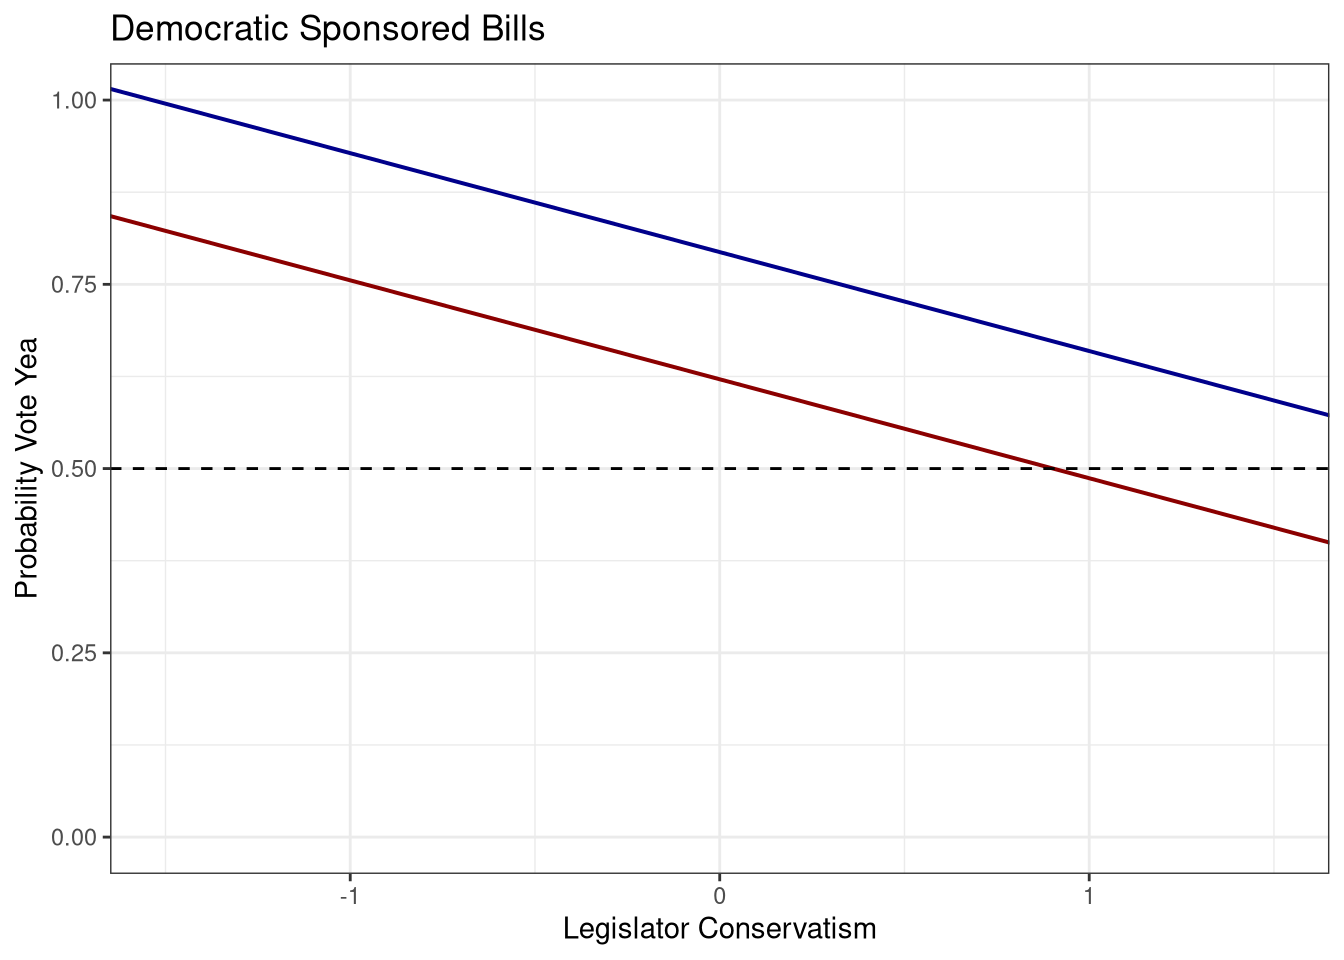
\includegraphics[width=0.5\linewidth]{Shor-Book_files/figure-latex/ideology-pred-1} 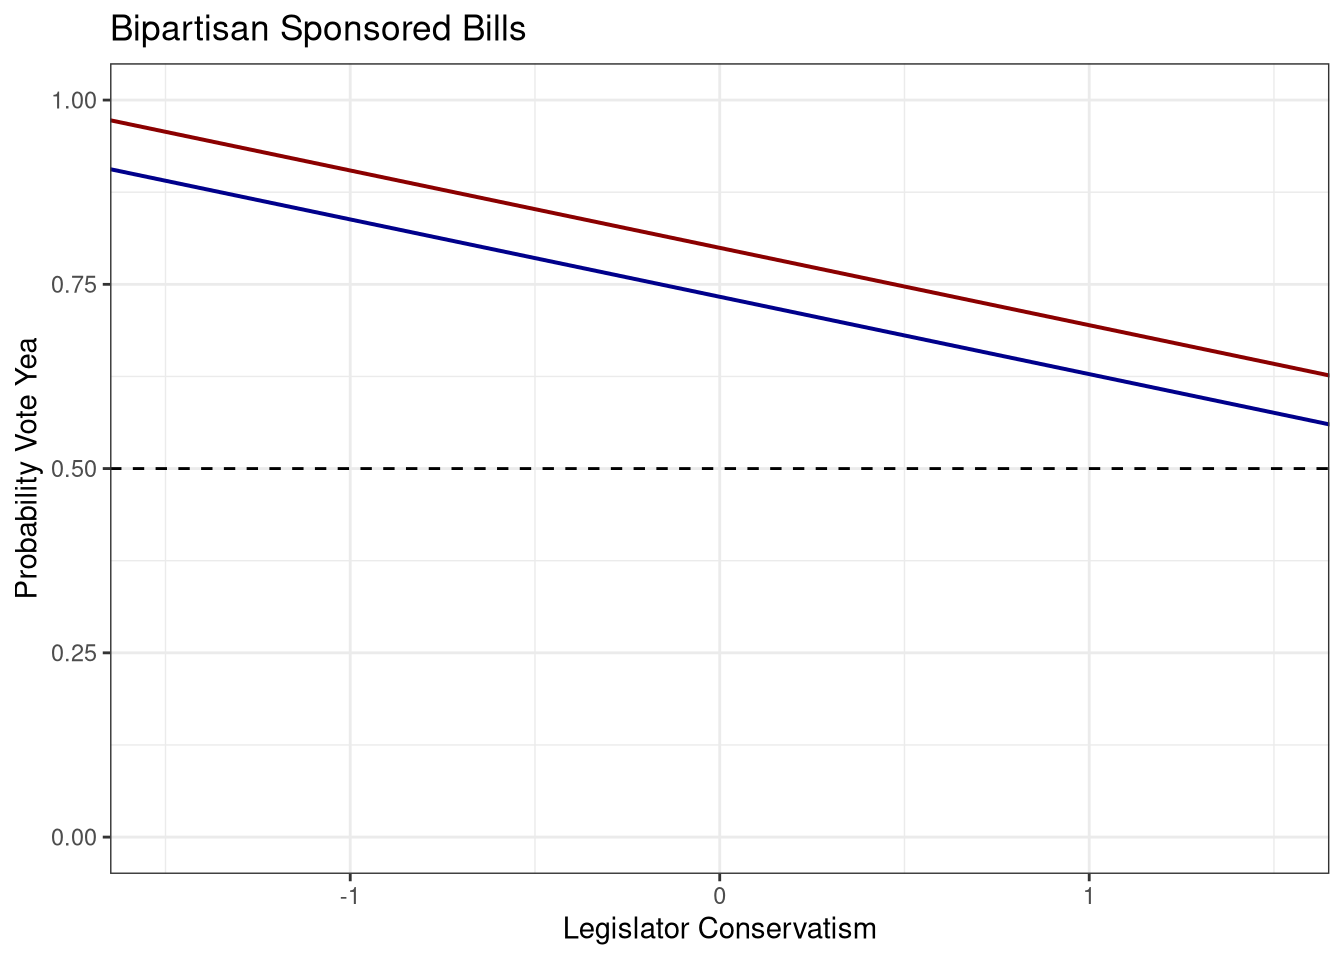
\includegraphics[width=0.5\linewidth]{Shor-Book_files/figure-latex/ideology-pred-2} 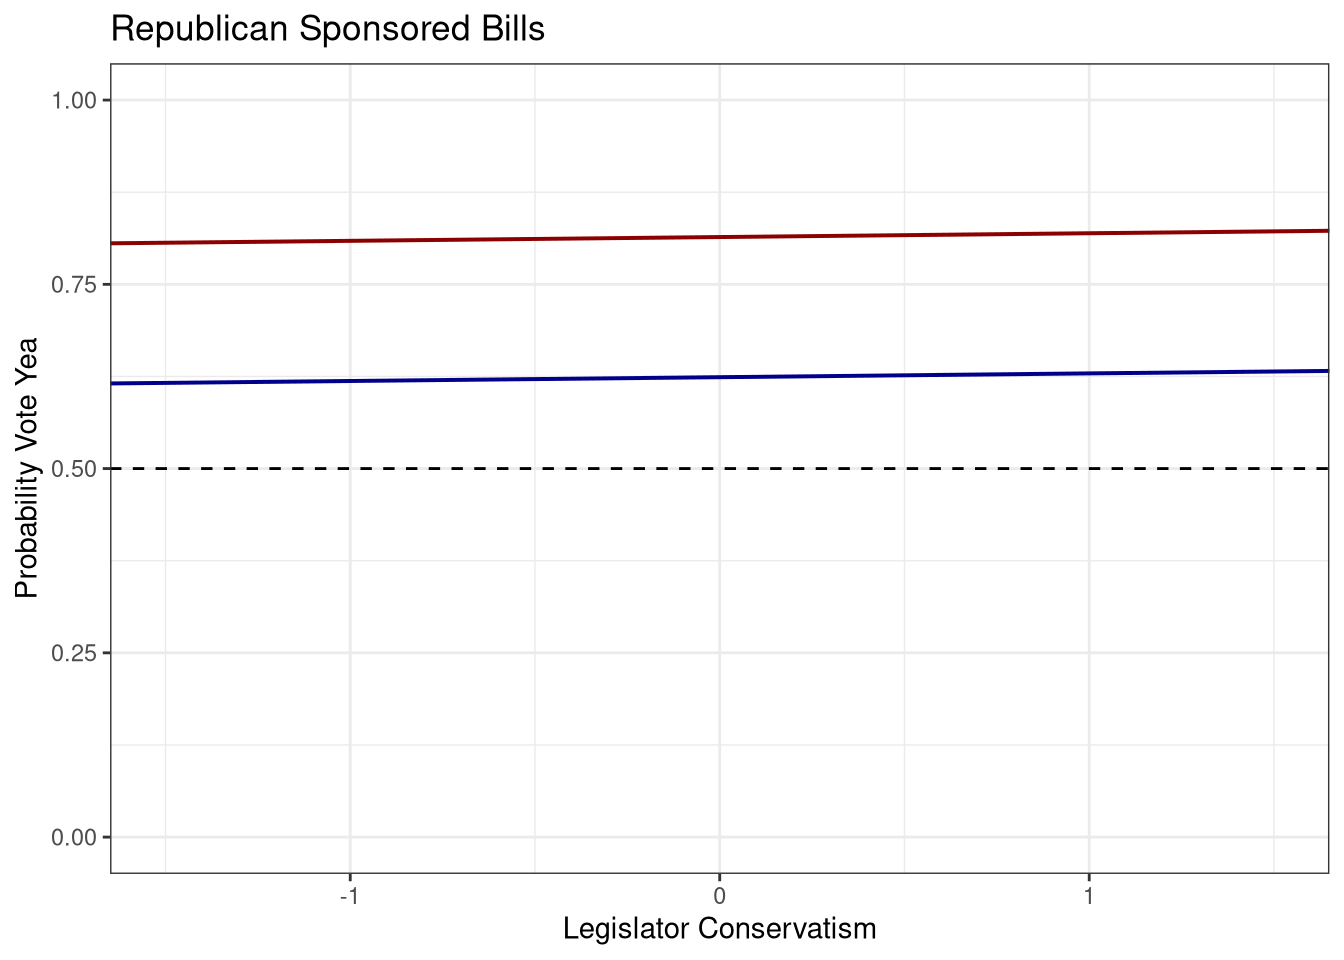
\includegraphics[width=0.5\linewidth]{Shor-Book_files/figure-latex/ideology-pred-3} \caption{Vote probability as a function of individual legislator ideology}\label{fig:ideology-pred}
\end{figure}

District ideology has no apparent effect on Democratic voting behavior, and a tiny one (in the expected direction) on Republican voting behavior.

  \bibliography{packages.bib,healthreforms.bib}

\end{document}
